\documentclass[hyperref={colorlinks = true},unknownkeysallowed]{beamer}
\usepackage{hyperref}%
\usepackage{graphicx} % graphics
\usepackage{epsfig} % eps graphics
\usepackage{booktabs, caption} % table styling
\usepackage{pgfplots}
\usepackage{amsmath}
\usepackage{tikz}
\usetikzlibrary{positioning}
\usetikzlibrary{fit}
\usetikzlibrary{backgrounds}
\usetikzlibrary{calc}
\usetikzlibrary{shapes}
\usetikzlibrary{mindmap}
\usetikzlibrary{decorations.text}
\usetikzlibrary{arrows.meta,arrows}
\usetikzlibrary{shapes.geometric}
\usepackage{changepage}
\usepackage{color}
\usepackage{caption}
\usepackage{transparent}
\usepackage{fontspec}
\usepackage{tcolorbox}
\usetikzlibrary{shapes}
\usepackage{natbib}
\usepackage{ifplatform}
\usefonttheme{professionalfonts} % using non standard fonts for beamer
\usefonttheme{serif} % default family is serif
\usefonttheme[onlymath]{serif}
\setmainfont{Helvetica Neue Light}

\linespread{1.3}

\bibliographystyle{plainnat}
\pgfplotsset{compat=1.7}

\makeatletter
\def\blfootnote{\xdef\@thefnmark{}\@footnotetext}
\makeatother

\definecolor{darkred}{rgb}{0.8,0,0}

%\definecolor{UBCblue}{rgb}{0.04706, 0.13725, 0.26667} % UBC Blue (primary)
\usecolortheme[named=darkred]{structure}

\let\oldbibitem=\bibitem
\renewcommand{\bibitem}[2][]{\label{#2}\oldbibitem[#1]{#2}}
\let\oldcite=\cite
\renewcommand\cite[1]{\hypersetup{linkcolor=darkred} \hyperlink{#1}{\oldcite{#1}}}
\let\oldcitep=\citep
\renewcommand\citep[1]{\hypersetup{linkcolor=darkred}\hyperlink{#1}{\oldcitep{#1}}}
\let\oldciteauthor=\citeauthor
\renewcommand\citeauthor[1]{\hypersetup{linkcolor=darkred}\hyperlink{#1}{\oldciteauthor{#1}}} 

\newenvironment{figure*}%
{\begin{figure}}
	{\end{figure}}

% suppress navigation bar
\beamertemplatenavigationsymbolsempty

\setbeamercolor{normal text}{fg=black}
\setbeamercolor{frametitle}{bg=white, fg=darkred}

\setbeamercolor{section title}{fg=black, bg=white}
\setbeamercolor{headline}{bg=white, fg=black}
\setbeamercolor*{palette primary}{fg=black,bg=black}
\setbeamercolor*{palette secondary}{fg=black,bg=black}
\setbeamercolor*{palette tertiary}{fg=black,bg=black}

\setbeamertemplate{itemize subitem}[triangle]




% see the macros.tex file for definitions
\usepackage{tikz}
\usepackage{xifthen}
\usepackage{xspace} %used at the end of macros to automatically determine whether spaces should be eaten or not
\usepackage[mathscr]{eucal} %use euler script instead of mathcal
\usepackage{dsfont} %doublestroke fonts (for things like reals, nats, complex numbers, etc)
\usepackage[nice]{nicefrac} %nice fraction typesetting, compact symbols for 1/2, etc

\usepackage{amsmath,amssymb,amsthm,bm,bbm,amsfonts,mathtools} %math
\usepackage[capitalize,sort,compress]{cleveref} %nice reference package for automatically choosing names for references
\DeclareMathAlphabet{\mathpzc}{OT1}{pzc}{m}{it}
\usepackage{import, subfiles} %packages for using subfile/folder structure
\usepackage{url} %nice URL typesetting
\usepackage[noend]{algpseudocode} 
\usepackage{algorithm} %typical alg typesetting packages
\usepackage{graphicx} %typical graphics package for figures
\usepackage{multirow} %multirow tables
\usepackage{wrapfig} %figures wrapped into the text
\usepackage{caption,subcaption} %package for sub-environments (figs, tables, etc)
\usepackage{microtype} %microtypesetting improvements for latex
\usepackage{booktabs} %professional quality tables
\usepackage{epigraph}
\usepackage{tcolorbox}
\usepackage{enumitem}
% adds reference to bottom right of corner of a slide
\usepackage[absolute,overlay]{textpos} % text references in slide corners
\newcommand\textref[1]{%
	\begin{textblock*}{\paperwidth}(0pt,0.99\textheight)
		\raggedleft \tiny{\emph{#1}}\hspace{.5em}
\end{textblock*}}

% for drawing circles around numbers
% ex. \circled{1} Add some text here.
\usepackage{tikz}
\newcommand*\circled[1]{\tikz[baseline=(char.base)]{
		\node[shape=circle,draw,inner sep=2pt] (char) {#1};}}
	
%%%%%%%%%%%%%%%%%%%%%%%%%%%%%%%%%%%
%%% Package Options Declarations %%
%%%%%%%%%%%%%%%%%%%%%%%%%%%%%%%%%%%
%hyperref format/color/etc
\DeclareOption{tchypersetup}{\hypersetup{colorlinks=true, allcolors=SubtleColor, pdfborder={0 0 0}}}
\DeclareOption{blackhypersetup}{\hypersetup{colorlinks=false, allcolors=black, pdfborder={0 0 0}}}
\def\boldorbar{\bar}
\DeclareOption{bbold}{\def\boldorbar{\bm}}
\DeclareOption{bbar}{\def\boldorbar{\bar}}
%autonum
\newif\ifuseautonum
\useautonumfalse
\DeclareOption{autonum}{\useautonumtrue}

\ProcessOptions

\ifuseautonum \usepackage{autonum} \fi

\definecolor{WowColor}{rgb}{.75,0,.75}
\definecolor{SubtleColor}{rgb}{0,0,.50}

% inline
\newcommand{\NA}[1]{\textcolor{SubtleColor}{ {\tiny \bf ($\star$)} #1}}
\newcommand{\LATER}[1]{\textcolor{SubtleColor}{ {\tiny \bf ($\dagger$)} #1}}
\newcommand{\TBD}[1]{\textcolor{SubtleColor}{ {\tiny \bf (!)} #1}}
\newcommand{\PROBLEM}[1]{\textcolor{WowColor}{ {\bf (!!)} {\bf #1}}}

% as margin notes
\newcounter{margincounter}
\newcommand{\displaycounter}{{\arabic{margincounter}}}
\newcommand{\incdisplaycounter}{{\stepcounter{margincounter}\arabic{margincounter}}}

\newcommand{\fTBD}[1]{\textcolor{SubtleColor}{$\,^{(\incdisplaycounter)}$}\marginpar{\tiny\textcolor{SubtleColor}{ {\tiny $(\displaycounter)$} #1}}}

\newcommand{\fPROBLEM}[1]{\textcolor{WowColor}{$\,^{((\incdisplaycounter))}$}\marginpar{\tiny\textcolor{WowColor}{ {\bf $\mathbf{((\displaycounter))}$} {\bf #1}}}}

\newcommand{\fLATER}[1]{\textcolor{SubtleColor}{$\,^{(\incdisplaycounter\dagger)}$}\marginpar{\tiny\textcolor{SubtleColor}{ {\tiny $(\displaycounter\dagger)$} #1}}}

\DeclareRobustCommand{\suppresscomments}{
	% For submission, make all render blank.
	\renewcommand{\LATER}[1]{}
	\renewcommand{\fLATER}[1]{}
	\renewcommand{\TBD}[1]{}
	\renewcommand{\fTBD}[1]{}
	\renewcommand{\PROBLEM}[1]{}
	\renewcommand{\fPROBLEM}[1]{}
	\renewcommand{\NA}[1]{##1}  %% Note, NA's pass through!
}

% shorten paper -- the higher shortenval, the shorter the paper
\newcommand{\setshortness}[1]{\def\shortnessval{#1}}
\setshortness{0}
\newcommand{\condcomment}[2][1]{\ifnum#1>\shortnessval #2\fi}

%%%%%%%%%%%%%
%%% Links %%%
%%%%%%%%%%%%%
\renewcommand*{\UrlFont}{\ttfamily\scriptsize\relax}

%%%%%%%%%%%%%%%%%%%%%%%%%%%%%%%%%%%%%%%
%%% Shortened \left/\right commands %%%
%%%%%%%%%%%%%%%%%%%%%%%%%%%%%%%%%%%%%%%
\def\l({\left(}
\def\r){\right)}
\def\l[{\left[}
\def\r]{\right]}
\def\lbr{\left\{}
\def\rbr{\right\}}

%%%%%%%%%%%%%%%%%%%%%%%
%%% Align shortcuts %%%
%%%%%%%%%%%%%%%%%%%%%%%
\AtBeginDocument{ %necessary to stop clash with autonum package
	\def\[#1\]{\begin{align}#1\end{align}}		% numbered
	\def \<#1\>{\begin{aligned}#1\end{aligned}}
	\def\(#1\){\begin{align*}#1\end{align*}} 	% unnumbered
}

% ******************************* Nomenclature *********************************
% To change the name of the Nomenclature section, uncomment the following line

%\renewcommand{\nomname}{Symbols}

\usepackage{bm}
\usepackage{xstring}
\usepackage{xpatch}
\usepackage{ragged2e}
\patchcmd{\thenomenclature}
{\leftmargin\labelwidth}
{\leftmargin\labelwidth\itemindent 1em }
{}{}

%%%%%%%%%%%%%%%%%%%%%%
%%% Important Sets %%%
%%%%%%%%%%%%%%%%%%%%%%
\newcommand{\reals}{\ensuremath{\mathbb{R}}}
\newcommand{\ints}{\ensuremath{\mathbb{Z}}}
\newcommand{\rats}{\ensuremath{\mathbb{Q}}}
\newcommand{\nats}{\ensuremath{\mathbb{N}}}
\newcommand{\comps}{\ensuremath{\mathbb{C}}}


%%%%%%%%%%%%%%%
%%% Vectors %%%
%%%%%%%%%%%%%%%
\newcommand{\bone}{\mathbf{1}}
\newcommand{\bzero}{\mathbf{0}}
\newcommand{\bell}{\mathbf{\ell}}


%%%%%%%%%%%%%%%%%%%%%%%%
%%% Matrix Operators %%%
%%%%%%%%%%%%%%%%%%%%%%%%
\newcommand{\diag}{\operatorname{diag}}
\newcommand{\tr}{\operatorname{tr}}
\newcommand{\kron}{\operatorname{\otimes}}


%%%%%%%%%%%%%%%%%%%%%%%
%%% General Purpose %%%
%%%%%%%%%%%%%%%%%%%%%%%
\newcommand{\tuple}[1][]{\left\langle #1 \right\rangle}
\newcommand{\emptystr}{\text{\o}}
\newcommand{\ind}{\mathds{1}} % indicator function
\newcommand{\sgn}{\operatorname{sgn}} % sign function
\newcommand{\theset}[1]{\lbrace #1 \rbrace}
\newcommand{\sn}[2]{\ensuremath{#1\!\times\!10^{#2}}}	% #1 x 10^{#2}

\newcommand{\st}{\,:\,}
\newcommand{\given}{\,|\,}
\newcommand{\closure}{\operatorname{cl}}
\newcommand{\spann}{\operatorname{span}}
\newcommand{\diam}{\operatorname{diam}}
\newcommand{\rank}{\operatorname{rank}}

% New definition of square root:
% it renames \sqrt as \oldsqrt
\let\oldsqrt\sqrt
% it defines the new \sqrt in terms of the old one
\def\sqrt{\mathpalette\DHLhksqrt}
\def\DHLhksqrt#1#2{%
	\setbox0=\hbox{$#1\oldsqrt{#2\,}$}\dimen0=\ht0
	\advance\dimen0-0.2\ht0
	\setbox2=\hbox{\vrule height\ht0 depth -\dimen0}%
	{\box0\lower0.4pt\box2}}

% min and max
\def\argmax{\operatornamewithlimits{arg\,max}}
\def\argmin{\operatornamewithlimits{arg\,min}}
\def\esssup{\operatornamewithlimits{ess\,sup}}
\def\essinf{\operatornamewithlimits{ess\,inf}}

% Equality operators
\mathtoolsset{centercolon}
%\newcommand{\defined}{\ensuremath{\triangleq}}
\newcommand{\defined}{:=}
\newcommand{\defines}{=:}
\newcommand{\xapprox}[1]{\underset{#1}{\approx}}
\newcommand{\medeq}{\!=\!}
\newcommand{\shorteq}{\!\!=\!\!}

% Other binary operators
\newcommand{\sm}{\!-\!}
\newcommand{\splus}{\!+\!}


%%%%%%%%%%%%%%%%%%%%%%%%%%%%%%%%%%
%%% Optimization               %%%
%%%%%%%%%%%%%%%%%%%%%%%%%%%%%%%%%%
\newcommand{\prox}[2]{\ensuremath{\operatorname{prox}_{#1}\left(#2\right)}}


%%%%%%%%%%%%%%%%%%%%%%%%%%%%%%%%%%
%%% Convex Analysis %%%
%%%%%%%%%%%%%%%%%%%%%%%%%%%%%%%%%%
\DeclareMathOperator{\cone}{cone}
\DeclareMathOperator{\conv}{conv}


%%%%%%%%%%%%%%%%%%%%%%%%%%%%%%%%%%
%%% Algorithms %%%
%%%%%%%%%%%%%%%%%%%%%%%%%%%%%%%%%%

%properly indented comments
%usage:
%\LineComment{X}{Here is the comment},  where X = # additional indents. 
%right after for / procedure / function calls, for whatever reason need to indent manually...
\newdimen{\algindent}
\setlength\algindent{1.5em}
\makeatletter
\newcommand{\LineComment}[2][0]{\Statex \hspace{#1\algindent} \hskip\ALG@thistlm $\triangleright$ #2}
\newcommand{\LineCommentIndent}[2][0]{\Statex \hspace{1.5em} \hskip\ALG@thistlm $\triangleright$ #2}
\makeatother

%%%%%%%%%%%%%%%%%%%%%%%%%%%%%%%%%%
%%% Probability and Statistics %%%
%%%%%%%%%%%%%%%%%%%%%%%%%%%%%%%%%%
% text shortcuts
\newcommand{\iid}{\textrm{i.i.d.}\@\xspace}
\newcommand{\as}{\textrm{a.s.}\@\xspace}
\newcommand{\aev}{\textrm{a.e.}\@\xspace}

% convergence
\newcommand{\convas}{\overset{a.s.}{\to}}
\newcommand{\convp}{\overset{p}{\to}}
\newcommand{\convd}{\overset{d}{\to}}
\newcommand{\eqd}{\overset{d}{=}}
\newcommand{\eqas}{\overset{a.s.}{=}}

% unary/functions
\renewcommand{\Pr}{\mathbb{P}}  % probability
\newcommand{\EE}{\mathbb{E}}	% expectation

\newcommand{\var}{\operatorname{Var}}	% variance
\newcommand{\cov}{\operatorname{Cov}}	% covariance
\newcommand{\corr}{\operatorname{Corr}}	% correlation
\newcommand{\supp}{\operatorname{supp}} %support

% binary operators
\newcommand{\dist}{\sim}
\newcommand{\distiid}{\overset{\textrm{\tiny\iid}}{\dist}}
\newcommand{\distind}{\overset{\textrm{\tiny\textrm{indep}}}{\dist}}

\def\independenT#1#2{\mathrel{\rlap{$#1#2$}\mkern4mu{#1#2}}}
\newcommand\indep{\protect\mathpalette{\protect\independenT}{\perp}} % independent

% parametric distributions
\newcommand{\distNamed}[1]{{\sf{#1}}}
\newcommand{\distNorm}{\mathcal{N}}
\newcommand{\distT}{\mathcal{T}}
\newcommand{\distLaplace}{\distNamed{Lap}}
%\newcommand{\distUnif}{\mathscr{U}}
\newcommand{\distUnif}{\distNamed{Unif}}
%\newcommand{\distGam}{\mathscr{G}{\scriptstyle\mathscr{A}}}
\newcommand{\distGam}{\distNamed{Gam}}
\newcommand{\distGumbel}{\distNamed{Gumbel}}
\newcommand{\distGEV}{\distNamed{GEV}}
\newcommand{\distCat}{\distNamed{Categorical}}
\newcommand{\distInvGam}{\distNamed{InvGam}}
%\newcommand{\distPoiss}{\mathscr{P}{\scriptstyle\mathscr{O}}}
\newcommand{\distPoiss}{\distNamed{Poiss}}
\newcommand{\distExp}{\distNamed{Exp}}
\newcommand{\distBeta}{\distNamed{Beta}}
\newcommand{\distBetaPrime}{\distNamed{Beta}'}
\newcommand{\distDir}{\distNamed{Dir}}
\newcommand{\distBinom}{\distNamed{Binom}}
\newcommand{\distMulti}{\distNamed{Multi}}
\newcommand{\distBern}{\distNamed{Bern}}
\newcommand{\distGeom}{\distNamed{Geom}}
\newcommand{\distWish}{\mathpzc{W}}
\newcommand{\distInvWish}{\mathpzc{IW}}
% non-parametric distribution
\newcommand{\distBeP}{\mathrm{BeP}}
\newcommand{\distDP}{\mathrm{DP}}
\newcommand{\distCRP}{\mathrm{CRP}}
\newcommand{\distPYP}{\mathrm{PY}}
\newcommand{\distGP}{{\mathrm{GP}}} % Gaussian process
\newcommand{\distPP}{\mathrm{PP}}
\newcommand{\distBP}{\mathrm{BP}}
\newcommand{\distBPP}{\mathrm{BPP}}
\newcommand{\distGammaP}{\mathrm{\Gamma P}}
\newcommand{\distNGammaP}{\mathrm{N\Gamma P}}
\newcommand{\distLP}{\mathrm{LP}}
\newcommand{\distObs}{\mathrm{Obs}}
\newcommand{\distCRM}{\mathrm{CRM}}
\newcommand{\distNCRM}{\mathrm{NCRM}}
\newcommand{\distVMF}{\mathrm{vMF}}


%%%%%%%%%%%%%%%%%%%%%%%%%%
%%% Information Theory %%%
%%%%%%%%%%%%%%%%%%%%%%%%%%
\newcommand{\divergence}[4][]{\mathrm{D^{\ifthenelse{\isempty{#1}}{}{#1}}_{#2}}\left(#3 || #4\right)}
\newcommand{\distance}[4][]{\mathrm{D^{\ifthenelse{\isempty{#1}}{}{#1}}_{#2}}\left(#3, #4\right)}
\newcommand{\crossent}[4][]{\mathrm{d^{\ifthenelse{\isempty{#1}}{}{#1}}_{#2}}\left(#3 || #4\right)}
\newcommand{\kl}[3][]{\divergence[#1]{KL}{#2}{#3}}
\newcommand{\tvd}[3][]{\distance[#1]{TV}{#2}{#3}}
\newcommand{\ent}[1]{\mathcal{H}\left(#1\right)}
\newcommand{\xent}[3][]{\crossent[#1]{KL}{#2}{#3}}
\newcommand{\db}[3][]{\crossent[#1]{\beta}{#2}{#3}}
\newcommand{\betadistance}[3][]{\divergence[#1]{\beta}{#2}{#3}}
\newcommand{\hell}[3][]{\distance[#1]{H}{#2}{#3}}
\newcommand{\plainkl}{\mathrm{D_{KL}}}
\newcommand{\hamming}{\mathrm{D_{H}}}
\newcommand{\plainxent}{\mathrm{d_{KL}}}
\newcommand{\plaindb}{\mathrm{d_{\beta}}}
\newcommand{\plainCapdb}{\mathrm{D_{\beta}}}
%%%%%%%%%%%%%%%%%%%%%%%%%%
%%% Variational Inference %%%
%%%%%%%%%%%%%%%%%%%%%%%%%%
\newcommand{\elbo}{\mathrm{ELBO}}

%%%%%%%%%%%%%%%%%%%%%
%%% Special Funcs %%%
%%%%%%%%%%%%%%%%%%%%%
\newcommand*\pFq[2]{{}_{#1}F_{#2}}

%%%%%%%%%%%%%%%%
%%% Calculus %%%
%%%%%%%%%%%%%%%%
\newcommand{\dee}{\mathrm{d}}
\newcommand{\grad}{\nabla}

\newcommand{\der}[2]{\ensuremath{\frac{\dee #1}{\dee #2}}}
\newcommand{\dder}[2]{\ensuremath{\frac{d^2 #1}{d #2^2}}}
\newcommand{\D}[2]{\ensuremath{\frac{\partial #1}{\partial #2}}}
\newcommand{\DD}[2]{\ensuremath{\frac{\partial^2 #1}{\partial #2^2}}}
\newcommand{\Di}[2]{\ensuremath{\frac{\partial^i #1}{\partial #2^i}}}
\newcommand{\prt}[1]{\ensuremath{\frac{\partial}{\partial #1}}}
\newcommand{\hes}[2]{\ensuremath{\frac{\partial^2}{\partial #1 \partial #2}}}


%%%%%%%%%%%%%
%%% Logic %%%
%%%%%%%%%%%%%
\DeclareMathOperator{\notimplies}{\centernot\implies}


%%%%%%%%%%%%%%%%%
%%% Fractions %%%
%%%%%%%%%%%%%%%%%
\newcommand{\half}{\ensuremath{\nicefrac{1}{2}}\xspace}
\newcommand{\third}{\ensuremath{\nicefrac{1}{3}}\xspace}
\newcommand{\quarter}{\ensuremath{\nicefrac{1}{4}}\xspace}


%%%%%%%%%%%%%%%%%
%%% Shortcuts %%%
%%%%%%%%%%%%%%%%%
\newcommand{\eps}{\epsilon}
\newcommand{\veps}{\varepsilon}
\newcommand{\bmat}{\begin{pmatrix}}
	\newcommand{\emat}{\end{pmatrix}}
\newcommand{\bitems}{\begin{itemize}}
	\newcommand{\eitems}{\end{itemize}}
\newcommand{\benum}{\begin{enumerate}}
	\newcommand{\eenum}{\end{enumerate}}
\newcommand{\bdesc}{\begin{description}}
	\newcommand{\edesc}{\end{description}}
\newcommand{\angles}[1]{\langle #1 \rangle}
\newcommand{\ip}[2]{\angles{#1, #2}}


%%%%%%%%%%%%%%
%%% Proofs %%%
%%%%%%%%%%%%%%
\newcommand{\bprf}{\begin{proof}}
	\newcommand{\eprf}{\end{proof}}
\newenvironment{proofof}[1]{\renewcommand{\proofname}{Proof of #1}\proof}{\endproof}
\newcommand{\bprfof}{\begin{proofof}}
	\newcommand{\eprfof}{\end{proofof}}


% Proof definitions
\theoremstyle{plain}
\newtheorem{nthm}{Theorem}
\newtheorem{nprop}[nthm]{Proposition}
\newtheorem{nlem}[nthm]{Lemma}
\newtheorem{ncor}[nthm]{Corollary}
\newtheorem{nconj}[nthm]{Conjecture}
\newtheorem*{thm}{Theorem}
\newtheorem*{stmt}{Statement}
\newtheorem*{prop}{Proposition}
\newtheorem*{lem}{Lemma}
\newtheorem*{cor}{Corollary}
\newtheorem*{conj}{Conjecture}

\theoremstyle{definition}
\newtheorem{ndefn}[nthm]{Definition}
\newtheorem{nexa}[nthm]{Example}
\newtheorem{nexer}[nthm]{Exercise}
\newtheorem{nassum}[nthm]{Assumption}
\newtheorem*{defn}{Definition}
\newtheorem*{exa}{Example}
\newtheorem*{exer}{Exercise}
\newtheorem*{cond}{Condition}
\newtheorem*{assum}{Assumption}

\theoremstyle{remark}
\newtheorem{nrmk}{Remark}
\newtheorem*{rmk}{Remark}
\newtheorem*{mynote}{Note}

% Proof shortcuts
\newcommand{\bthm}{\begin{thm}}
	\newcommand{\ethm}{\end{thm}}
\newcommand{\bnthm}{\begin{nthm}}
	\newcommand{\enthm}{\end{nthm}}

\newcommand{\bnprop}{\begin{nprop}}
	\newcommand{\enprop}{\end{nprop}}
\newcommand{\bprop}{\begin{prop}}
	\newcommand{\eprop}{\end{prop}}

\newcommand{\bnlem}{\begin{nlem}}
	\newcommand{\enlem}{\end{nlem}}
\newcommand{\blem}{\begin{lem}}
	\newcommand{\elem}{\end{lem}}

\newcommand{\bncor}{\begin{ncor}}
	\newcommand{\encor}{\end{ncor}}
\newcommand{\bcor}{\begin{cor}}
	\newcommand{\ecor}{\end{cor}}

\newcommand{\bnconj}{\begin{nconj}}
	\newcommand{\enconj}{\end{nconj}}
\newcommand{\bconj}{\begin{conj}}
	\newcommand{\econj}{\end{conj}}

\newcommand{\bnumdefn}{\begin{ndefn}}
	\newcommand{\enumdefn}{\end{ndefn}}
\newcommand{\bdefn}{\begin{defn}}
	\newcommand{\edefn}{\end{defn}}

\newcommand{\bnexa}{\begin{nexa}}
	\newcommand{\enexa}{\end{nexa}}
\newcommand{\bexa}{\begin{exa}}
	\newcommand{\eexa}{\end{exa}}

\newcommand{\bnexer}{\begin{nexer}}
	\newcommand{\enexer}{\end{nexer}}
\newcommand{\bexer}{\begin{exer}}
	\newcommand{\eexer}{\end{exer}}

\newcommand{\bnassum}{\begin{nassum}}
	\newcommand{\enassum}{\end{nassum}}
\newcommand{\bassum}{\begin{assum}}
	\newcommand{\eassum}{\end{assum}}

\newcommand{\bcond}{\begin{cond}}
	\newcommand{\econd}{\end{cond}}

\newcommand{\bnrmk}{\begin{nrmk}}
	\newcommand{\enrmk}{\end{nrmk}}
\newcommand{\brmk}{\begin{rmk}}
	\newcommand{\ermk}{\end{rmk}}
\newcommand{\bnote}{\begin{mynote}}
	\newcommand{\enote}{\end{mynote}}

%Proof clever ref names
\crefname{nlem}{Lemma}{Lemmas}
\crefname{nprop}{Proposition}{Propositions}
\crefname{ncor}{Corollary}{Corollaries}
\crefname{nthm}{Theorem}{Theorems}
\crefname{nexa}{Example}{Examples}
\crefname{ndefn}{Definition}{Definitions}
\crefname{nassum}{Assumption}{Assumptions}
\crefformat{footnote}{#1\footnotemark[#2]#3}


%%%%%%%%%%%%%%%%%%%%%%%%
%%% Symbol shortcuts %%%
%%%%%%%%%%%%%%%%%%%%%%%%

% Math bold italics
\def\mathbbi#1{\textbf{\em #1}}


% Bar everything shortcuts
\newcommand{\barA}{\bar{A}}
\newcommand{\barB}{\bar{B}}
\newcommand{\barC}{\bar{C}}
\newcommand{\barD}{\bar{D}}
\newcommand{\barE}{\bar{E}}
\newcommand{\barF}{\bar{F}}
\newcommand{\barG}{\bar{G}}
\newcommand{\barH}{\bar{H}}
\newcommand{\barI}{\bar{I}}
\newcommand{\barJ}{\bar{J}}
\newcommand{\barK}{\bar{K}}
\newcommand{\barL}{\bar{L}}
\newcommand{\barM}{\bar{M}}
\newcommand{\barN}{\bar{N}}
\newcommand{\barO}{\bar{O}}
\newcommand{\barP}{\bar{P}}
\newcommand{\barQ}{\bar{Q}}
\newcommand{\barR}{\bar{R}}
\newcommand{\barS}{\bar{S}}
\newcommand{\barT}{\bar{T}}
\newcommand{\barU}{\bar{U}}
\newcommand{\barV}{\bar{V}}
\newcommand{\barW}{\bar{W}}
\newcommand{\barX}{\bar{X}}
\newcommand{\barY}{\bar{Y}}
\newcommand{\barZ}{\bar{Z}}
\newcommand{\bara}{\bar{a}}
\newcommand{\barb}{\bar{b}}
\newcommand{\barc}{\bar{c}}
\newcommand{\bard}{\bar{d}}
\newcommand{\bare}{\bar{e}}
\newcommand{\barf}{\bar{f}}
\newcommand{\barg}{\bar{g}}
\newcommand{\barh}{\bar{h}}
\newcommand{\bari}{\bar{i}}
\newcommand{\barj}{\bar{j}}
\newcommand{\bark}{\bar{k}}
\newcommand{\barl}{\bar{l}}
\newcommand{\barm}{\bar{m}}
\newcommand{\barn}{\bar{n}}
\newcommand{\baro}{\bar{o}}
\newcommand{\barp}{\bar{p}}
\newcommand{\barq}{\bar{q}}
\newcommand{\barr}{\bar{r}}
\newcommand{\bars}{\bar{s}}
\newcommand{\bart}{\bar{t}}
\newcommand{\baru}{\bar{u}}
\newcommand{\barv}{\bar{v}}
\newcommand{\barw}{\bar{w}}
\newcommand{\barx}{\bar{x}}
\newcommand{\bary}{\bar{y}}
\newcommand{\barz}{\bar{z}}


\newcommand{\bA}{\boldorbar{A}}
\newcommand{\bB}{\boldorbar{B}}
\newcommand{\bC}{\boldorbar{C}}
\newcommand{\bD}{\boldorbar{D}}
\newcommand{\bE}{\boldorbar{E}}
\newcommand{\bF}{\boldorbar{F}}
\newcommand{\bG}{\boldorbar{G}}
\newcommand{\bH}{\boldorbar{H}}
\newcommand{\bI}{\boldorbar{I}}
\newcommand{\bJ}{\boldorbar{J}}
\newcommand{\bK}{\boldorbar{K}}
\newcommand{\bL}{\boldorbar{L}}
\newcommand{\bM}{\boldorbar{M}}
\newcommand{\bN}{\boldorbar{N}}
\newcommand{\bO}{\boldorbar{O}}
\newcommand{\bP}{\boldorbar{P}}
\newcommand{\bQ}{\boldorbar{Q}}
\newcommand{\bR}{\boldorbar{R}}
\newcommand{\bS}{\boldorbar{S}}
\newcommand{\bT}{\boldorbar{T}}
\newcommand{\bU}{\boldorbar{U}}
\newcommand{\bV}{\boldorbar{V}}
\newcommand{\bW}{\boldorbar{W}}
\newcommand{\bX}{\boldorbar{X}}
\newcommand{\bY}{\boldorbar{Y}}
\newcommand{\bZ}{\boldorbar{Z}}
\newcommand{\ba}{\boldorbar{a}}
\newcommand{\bb}{\boldorbar{b}}
\newcommand{\bc}{\boldorbar{c}}
\newcommand{\bd}{\boldorbar{d}}
\newcommand{\be}{\boldorbar{e}}
\newcommand{\bbf}{\boldorbar{f}}
\newcommand{\bg}{\boldorbar{g}}
\newcommand{\bh}{\boldorbar{h}}
\newcommand{\bi}{\boldorbar{i}}
\newcommand{\bj}{\boldorbar{j}}
\newcommand{\bk}{\boldorbar{k}}
\newcommand{\bl}{\boldorbar{l}}
%\newcommand{\bm}{\boldorbar{m}}
\newcommand{\bn}{\boldorbar{n}}
\newcommand{\bo}{\boldorbar{o}}
\newcommand{\bp}{\boldorbar{p}}
\newcommand{\bq}{\boldorbar{q}}
\newcommand{\br}{\boldorbar{r}}
\newcommand{\bs}{\boldorbar{s}}
\newcommand{\bt}{\boldorbar{t}}
\newcommand{\bu}{\boldorbar{u}}
\newcommand{\bv}{\boldorbar{v}}
\newcommand{\bw}{\boldorbar{w}}
\newcommand{\bx}{\boldorbar{x}}
\newcommand{\by}{\boldorbar{y}}
\newcommand{\bz}{\boldorbar{z}}

\newcommand{\balpha}{\boldorbar{\alpha}}
\newcommand{\bbeta}{\boldorbar{\beta}}
\newcommand{\bepsilon}{\boldorbar{\epsilon}}
\newcommand{\boldeta}{\boldorbar{\eta}}
\newcommand{\bkappa}{\boldorbar{\kappa}}
\newcommand{\bgamma}{\boldorbar{\gamma}}
\newcommand{\blambda}{\boldorbar{\lambda}}
\newcommand{\bomega}{\boldorbar{\omega}}
\newcommand{\bmu}{\boldorbar{\mu}}
\newcommand{\bpi}{\boldorbar{\pi}}
\newcommand{\bphi}{\boldorbar{\phi}}
\newcommand{\bpsi}{\boldorbar{\psi}}
\newcommand{\bsigma}{\boldorbar{\sigma}}
\newcommand{\btheta}{\boldorbar{\theta}}
\newcommand{\bxi}{\boldorbar{\xi}}
\newcommand{\bzeta}{\boldorbar{\zeta}}
\newcommand{\bGamma}{\boldorbar{\Gamma}}
\newcommand{\bLambda}{\boldorbar{\Lambda}}
\newcommand{\bOmega}{\boldorbar{\Omega}}
\newcommand{\bPhi}{\boldorbar{\Phi}}
\newcommand{\bPi}{\boldorbar{\Pi}}
\newcommand{\bPsi}{\boldorbar{\Psi}}
\newcommand{\bSigma}{\boldorbar{\Sigma}}
\newcommand{\bTheta}{\boldorbar{\Theta}}
\newcommand{\bUpsilon}{\boldorbar{\Upsilon}}
\newcommand{\bXi}{\boldorbar{\Xi}}

% Mathcal shortcuts
\newcommand{\mcA}{\mathcal{A}}
\newcommand{\mcB}{\mathcal{B}}
\newcommand{\mcC}{\mathcal{C}}
\newcommand{\mcD}{\mathcal{D}}
\newcommand{\mcE}{\mathcal{E}}
\newcommand{\mcF}{\mathcal{F}}
\newcommand{\mcG}{\mathcal{G}}
\newcommand{\mcH}{\mathcal{H}}
\newcommand{\mcI}{\mathcal{I}}
\newcommand{\mcJ}{\mathcal{J}}
\newcommand{\mcK}{\mathcal{K}}
\newcommand{\mcL}{\mathcal{L}}
\newcommand{\mcM}{\mathcal{M}}
\newcommand{\mcN}{\mathcal{N}}
\newcommand{\mcO}{\mathcal{O}}
\newcommand{\mcP}{\mathcal{P}}
\newcommand{\mcQ}{\mathcal{Q}}
\newcommand{\mcR}{\mathcal{R}}
\newcommand{\mcS}{\mathcal{S}}
\newcommand{\mcT}{\mathcal{T}}
\newcommand{\mcU}{\mathcal{U}}
\newcommand{\mcV}{\mathcal{V}}
\newcommand{\mcW}{\mathcal{W}}
\newcommand{\mcX}{\mathcal{X}}
\newcommand{\mcY}{\mathcal{Y}}
\newcommand{\mcZ}{\mathcal{Z}}
\newcommand{\mcPsi}{\mathcal{\Psi}}

\newcommand{\hmcA}{\hat{\mathcal{A}}}
\newcommand{\hmcB}{\hat{\mathcal{B}}}
\newcommand{\hmcC}{\hat{\mathcal{C}}}
\newcommand{\hmcD}{\hat{\mathcal{D}}}
\newcommand{\hmcE}{\hat{\mathcal{E}}}
\newcommand{\hmcF}{\hat{\mathcal{F}}}
\newcommand{\hmcG}{\hat{\mathcal{G}}}
\newcommand{\hmcH}{\hat{\mathcal{H}}}
\newcommand{\hmcI}{\hat{\mathcal{I}}}
\newcommand{\hmcJ}{\hat{\mathcal{J}}}
\newcommand{\hmcK}{\hat{\mathcal{K}}}
\newcommand{\hmcL}{\hat{\mathcal{L}}}
\newcommand{\hmcM}{\hat{\mathcal{M}}}
\newcommand{\hmcN}{\hat{\mathcal{N}}}
\newcommand{\hmcO}{\hat{\mathcal{O}}}
\newcommand{\hmcP}{\hat{\mathcal{P}}}
\newcommand{\hmcQ}{\hat{\mathcal{Q}}}
\newcommand{\hmcR}{\hat{\mathcal{R}}}
\newcommand{\hmcS}{\hat{\mathcal{S}}}
\newcommand{\hmcT}{\hat{\mathcal{T}}}
\newcommand{\hmcU}{\hat{\mathcal{U}}}
\newcommand{\hmcV}{\hat{\mathcal{V}}}
\newcommand{\hmcW}{\hat{\mathcal{W}}}
\newcommand{\hmcX}{\hat{\mathcal{X}}}
\newcommand{\hmcY}{\hat{\mathcal{Y}}}
\newcommand{\hmcZ}{\hat{\mathcal{Z}}}

% Mathfrak shortcuts
\newcommand{\mfA}{\mathfrak{A}}
\newcommand{\mfB}{\mathfrak{B}}
\newcommand{\mfC}{\mathfrak{C}}
\newcommand{\mfD}{\mathfrak{D}}
\newcommand{\mfE}{\mathfrak{E}}
\newcommand{\mfF}{\mathfrak{F}}
\newcommand{\mfG}{\mathfrak{G}}
\newcommand{\mfH}{\mathfrak{H}}
\newcommand{\mfI}{\mathfrak{I}}
\newcommand{\mfJ}{\mathfrak{J}}
\newcommand{\mfK}{\mathfrak{K}}
\newcommand{\mfL}{\mathfrak{L}}
\newcommand{\mfM}{\mathfrak{M}}
\newcommand{\mfN}{\mathfrak{N}}
\newcommand{\mfO}{\mathfrak{O}}
\newcommand{\mfP}{\mathfrak{P}}
\newcommand{\mfQ}{\mathfrak{Q}}
\newcommand{\mfR}{\mathfrak{R}}
\newcommand{\mfS}{\mathfrak{S}}
\newcommand{\mfT}{\mathfrak{T}}
\newcommand{\mfU}{\mathfrak{U}}
\newcommand{\mfV}{\mathfrak{V}}
\newcommand{\mfW}{\mathfrak{W}}
\newcommand{\mfX}{\mathfrak{X}}
\newcommand{\mfY}{\mathfrak{Y}}
\newcommand{\mfZ}{\mathfrak{Z}}
\newcommand{\mfa}{\mathfrak{a}}
\newcommand{\mfb}{\mathfrak{b}}
\newcommand{\mfc}{\mathfrak{c}}
\newcommand{\mfd}{\mathfrak{d}}
\newcommand{\mfe}{\mathfrak{e}}
\newcommand{\mff}{\mathfrak{f}}
\newcommand{\mfg}{\mathfrak{g}}
\newcommand{\mfh}{\mathfrak{h}}
\newcommand{\mfi}{\mathfrak{i}}
\newcommand{\mfj}{\mathfrak{j}}
\newcommand{\mfk}{\mathfrak{k}}
\newcommand{\mfl}{\mathfrak{l}}
\newcommand{\mfm}{\mathfrak{m}}
\newcommand{\mfn}{\mathfrak{n}}
\newcommand{\mfo}{\mathfrak{o}}
\newcommand{\mfp}{\mathfrak{p}}
\newcommand{\mfq}{\mathfrak{q}}
\newcommand{\mfr}{\mathfrak{r}}
\newcommand{\mfs}{\mathfrak{s}}
\newcommand{\mft}{\mathfrak{t}}
\newcommand{\mfu}{\mathfrak{u}}
\newcommand{\mfv}{\mathfrak{v}}
\newcommand{\mfw}{\mathfrak{w}}
\newcommand{\mfx}{\mathfrak{x}}
\newcommand{\mfy}{\mathfrak{y}}
\newcommand{\mfz}{\mathfrak{z}}

% Bold Mathfrak shortcuts
\newcommand{\bmfA}{\mathbf{\mathfrak{A}}}
\newcommand{\bmfB}{\mathbf{\mathfrak{B}}}
\newcommand{\bmfC}{\mathbf{\mathfrak{C}}}
\newcommand{\bmfD}{\mathbf{\mathfrak{D}}}
\newcommand{\bmfE}{\mathbf{\mathfrak{E}}}
\newcommand{\bmfF}{\mathbf{\mathfrak{F}}}
\newcommand{\bmfG}{\mathbf{\mathfrak{G}}}
\newcommand{\bmfH}{\mathbf{\mathfrak{H}}}
\newcommand{\bmfI}{\mathbf{\mathfrak{I}}}
\newcommand{\bmfJ}{\mathbf{\mathfrak{J}}}
\newcommand{\bmfK}{\mathbf{\mathfrak{K}}}
\newcommand{\bmfL}{\mathbf{\mathfrak{L}}}
\newcommand{\bmfM}{\mathbf{\mathfrak{M}}}
\newcommand{\bmfN}{\mathbf{\mathfrak{N}}}
\newcommand{\bmfO}{\mathbf{\mathfrak{O}}}
\newcommand{\bmfP}{\mathbf{\mathfrak{P}}}
\newcommand{\bmfQ}{\mathbf{\mathfrak{Q}}}
\newcommand{\bmfR}{\mathbf{\mathfrak{R}}}
\newcommand{\bmfS}{\mathbf{\mathfrak{S}}}
\newcommand{\bmfT}{\mathbf{\mathfrak{T}}}
\newcommand{\bmfU}{\mathbf{\mathfrak{U}}}
\newcommand{\bmfV}{\mathbf{\mathfrak{V}}}
\newcommand{\bmfW}{\mathbf{\mathfrak{W}}}
\newcommand{\bmfX}{\mathbf{\mathfrak{X}}}
\newcommand{\bmfY}{\mathbf{\mathfrak{Y}}}
\newcommand{\bmfZ}{\mathbf{\mathfrak{Z}}}
\newcommand{\bmfa}{\mathbf{\mathfrak{a}}}
\newcommand{\bmfb}{\mathbf{\mathfrak{b}}}
\newcommand{\bmfc}{\mathbf{\mathfrak{c}}}
\newcommand{\bmfd}{\mathbf{\mathfrak{d}}}
\newcommand{\bmfe}{\mathbf{\mathfrak{e}}}
\newcommand{\bmff}{\mathbf{\mathfrak{f}}}
\newcommand{\bmfg}{\mathbf{\mathfrak{g}}}
\newcommand{\bmfh}{\mathbf{\mathfrak{h}}}
\newcommand{\bmfi}{\mathbf{\mathfrak{i}}}
\newcommand{\bmfj}{\mathbf{\mathfrak{j}}}
\newcommand{\bmfk}{\mathbf{\mathfrak{k}}}
\newcommand{\bmfl}{\mathbf{\mathfrak{l}}}
\newcommand{\bmfm}{\mathbf{\mathfrak{m}}}
\newcommand{\bmfn}{\mathbf{\mathfrak{n}}}
\newcommand{\bmfo}{\mathbf{\mathfrak{o}}}
\newcommand{\bmfp}{\mathbf{\mathfrak{p}}}
\newcommand{\bmfq}{\mathbf{\mathfrak{q}}}
\newcommand{\bmfr}{\mathbf{\mathfrak{r}}}
\newcommand{\bmfs}{\mathbf{\mathfrak{s}}}
\newcommand{\bmft}{\mathbf{\mathfrak{t}}}
\newcommand{\bmfu}{\mathbf{\mathfrak{u}}}
\newcommand{\bmfv}{\mathbf{\mathfrak{v}}}
\newcommand{\bmfw}{\mathbf{\mathfrak{w}}}
\newcommand{\bmfx}{\mathbf{\mathfrak{x}}}
\newcommand{\bmfy}{\mathbf{\mathfrak{y}}}
\newcommand{\bmfz}{\mathbf{\mathfrak{z}}}

% Hatted shortcuts
\newcommand{\hA}{\hat{A}}
\newcommand{\hB}{\hat{B}}
\newcommand{\hC}{\hat{C}}
\newcommand{\hD}{\hat{D}}
\newcommand{\hE}{\hat{E}}
\newcommand{\hF}{\hat{F}}
\newcommand{\hG}{\hat{G}}
\newcommand{\hH}{\hat{H}}
\newcommand{\hI}{\hat{I}}
\newcommand{\hJ}{\hat{J}}
\newcommand{\hK}{\hat{K}}
\newcommand{\hL}{\hat{L}}
\newcommand{\hM}{\hat{M}}
\newcommand{\hN}{\hat{N}}
\newcommand{\hO}{\hat{O}}
\newcommand{\hP}{\hat{P}}
\newcommand{\hQ}{\hat{Q}}
\newcommand{\hR}{\hat{R}}
\newcommand{\hS}{\hat{S}}
\newcommand{\hT}{\hat{T}}
\newcommand{\hU}{\hat{U}}
\newcommand{\hV}{\hat{V}}
\newcommand{\hW}{\hat{W}}
\newcommand{\hX}{\hat{X}}
\newcommand{\hY}{\hat{Y}}
\newcommand{\hZ}{\hat{Z}}
\newcommand{\ha}{\hat{a}}
\newcommand{\hh}{\hat{h}}
\newcommand{\hc}{\hat{c}}
\newcommand{\hd}{\hat{d}}
\newcommand{\he}{\hat{e}}
\newcommand{\hf}{\hat{f}}
\newcommand{\hg}{\hat{g}}
\newcommand{\Hh}{\hat{h}} %% NB
\newcommand{\hi}{\hat{i}}
\newcommand{\hj}{\hat{j}}
\newcommand{\hk}{\hat{k}}
\newcommand{\hl}{\hat{l}}
%\newcommand{\hm}{\hat{m}}
\newcommand{\hn}{\hat{n}}
\newcommand{\ho}{\hat{o}}
\newcommand{\hp}{\hat{p}}
\newcommand{\hq}{\hat{q}}
\newcommand{\hr}{\hat{r}}
\newcommand{\hs}{\hat{s}}
\newcommand{\Ht}{\hat{t}} %% NB
\newcommand{\hu}{\hat{u}}
\newcommand{\hv}{\hat{v}}
\newcommand{\hw}{\hat{w}}
\newcommand{\hx}{\hat{x}}
\newcommand{\hy}{\hat{y}}
\newcommand{\hz}{\hat{z}}

% Bold hatted shortcuts
\newcommand{\bhA}{\mathbf{\hat{A}}}
\newcommand{\bhB}{\mathbf{\hat{B}}}
\newcommand{\bhC}{\mathbf{\hat{C}}}
\newcommand{\bhD}{\mathbf{\hat{D}}}
\newcommand{\bhE}{\mathbf{\hat{E}}}
\newcommand{\bhF}{\mathbf{\hat{F}}}
\newcommand{\bhG}{\mathbf{\hat{G}}}
\newcommand{\bhH}{\mathbf{\hat{H}}}
\newcommand{\bhI}{\mathbf{\hat{I}}}
\newcommand{\bhJ}{\mathbf{\hat{J}}}
\newcommand{\bhK}{\mathbf{\hat{K}}}
\newcommand{\bhL}{\mathbf{\hat{L}}}
\newcommand{\bhM}{\mathbf{\hat{M}}}
\newcommand{\bhN}{\mathbf{\hat{N}}}
\newcommand{\bhO}{\mathbf{\hat{O}}}
\newcommand{\bhP}{\mathbf{\hat{P}}}
\newcommand{\bhQ}{\mathbf{\hat{Q}}}
\newcommand{\bhR}{\mathbf{\hat{R}}}
\newcommand{\bhS}{\mathbf{\hat{S}}}
\newcommand{\bhT}{\mathbf{\hat{T}}}
\newcommand{\bhU}{\mathbf{\hat{U}}}
\newcommand{\bhV}{\mathbf{\hat{V}}}
\newcommand{\bhW}{\mathbf{\hat{W}}}
\newcommand{\bhX}{\mathbf{\hat{X}}}
\newcommand{\bhY}{\mathbf{\hat{Y}}}
\newcommand{\bhZ}{\mathbf{\hat{Z}}}
\newcommand{\bha}{\mathbf{\hat{a}}}
\newcommand{\bhh}{\mathbf{\hat{h}}}
\newcommand{\bhc}{\mathbf{\hat{c}}}
\newcommand{\bhd}{\mathbf{\hat{d}}}
\newcommand{\bhe}{\mathbf{\hat{e}}}
\newcommand{\bhf}{\mathbf{\hat{f}}}
\newcommand{\bhg}{\mathbf{\hat{g}}}
\newcommand{\Bhh}{\mathbf{\hat{h}}}
\newcommand{\bhi}{\mathbf{\hat{i}}}
\newcommand{\bhj}{\mathbf{\hat{j}}}
\newcommand{\bhk}{\mathbf{\hat{k}}}
\newcommand{\bhl}{\mathbf{\hat{l}}}
\newcommand{\bhm}{\mathbf{\hat{m}}}
\newcommand{\bhn}{\mathbf{\hat{n}}}
\newcommand{\bho}{\mathbf{\hat{o}}}
\newcommand{\bhp}{\mathbf{\hat{p}}}
\newcommand{\bhq}{\mathbf{\hat{q}}}
\newcommand{\bhr}{\mathbf{\hat{r}}}
\newcommand{\bhs}{\mathbf{\hat{s}}}
\newcommand{\bht}{\mathbf{\hat{t}}}
\newcommand{\bhu}{\mathbf{\hat{u}}}
\newcommand{\bhv}{\mathbf{\hat{v}}}
\newcommand{\bhw}{\mathbf{\hat{w}}}
\newcommand{\bhx}{\mathbf{\hat{x}}}
\newcommand{\bhy}{\mathbf{\hat{y}}}
\newcommand{\bhz}{\mathbf{\hat{z}}}

% Tilde shortcuts
\newcommand{\tA}{\tilde{A}}
\newcommand{\tB}{\tilde{B}}
\newcommand{\tC}{\tilde{C}}
\newcommand{\tD}{\tilde{D}}
\newcommand{\tE}{\tilde{E}}
\newcommand{\tF}{\tilde{F}}
\newcommand{\tG}{\tilde{G}}
\newcommand{\tH}{\tilde{H}}
\newcommand{\tI}{\tilde{I}}
\newcommand{\tJ}{\tilde{J}}
\newcommand{\tK}{\tilde{K}}
\newcommand{\tL}{\tilde{L}}
\newcommand{\tM}{\tilde{M}}
\newcommand{\tN}{\tilde{N}}
\newcommand{\tO}{\tilde{O}}
\newcommand{\tP}{\tilde{P}}
\newcommand{\tQ}{\tilde{Q}}
\newcommand{\tR}{\tilde{R}}
\newcommand{\tS}{\tilde{S}}
\newcommand{\tT}{\tilde{T}}
\newcommand{\tU}{\tilde{U}}
\newcommand{\tV}{\tilde{V}}
\newcommand{\tW}{\tilde{W}}
\newcommand{\tX}{\tilde{X}}
\newcommand{\tY}{\tilde{Y}}
\newcommand{\tZ}{\tilde{Z}}
\newcommand{\ta}{\tilde{a}}
\newcommand{\tth}{\tilde{h}}
%\newcommand{\tc}{\tilde{c}}
\newcommand{\td}{\tilde{d}}
\newcommand{\te}{\tilde{e}}
\newcommand{\tf}{\tilde{f}}
\newcommand{\tg}{\tilde{g}}
\newcommand{\tildeh}{\tilde{h}}
\newcommand{\ti}{\tilde{i}}
\newcommand{\tj}{\tilde{j}}
\newcommand{\tk}{\tilde{k}}
\newcommand{\tl}{\tilde{l}}
\newcommand{\tm}{\tilde{m}}
\newcommand{\tn}{\tilde{n}}
%\newcommand{\tto}{\tilde{o}}
\newcommand{\tp}{\tilde{p}}
\newcommand{\tq}{\tilde{q}}
%\newcommand{\tr}{\tilde{r}}
\newcommand{\ts}{\tilde{s}}
%\newcommand{\tt}{\tilde{t}}
\newcommand{\tu}{\tilde{u}}
\newcommand{\tv}{\tilde{v}}
\newcommand{\tw}{\tilde{w}}
\newcommand{\tx}{\tilde{x}}
\newcommand{\ty}{\tilde{y}}
\newcommand{\tz}{\tilde{z}}

% Bold tilde shortcuts
\newcommand{\btA}{\mathbf{\tilde{A}}}
\newcommand{\btB}{\mathbf{\tilde{B}}}
\newcommand{\btC}{\mathbf{\tilde{C}}}
\newcommand{\btD}{\mathbf{\tilde{D}}}
\newcommand{\btE}{\mathbf{\tilde{E}}}
\newcommand{\btF}{\mathbf{\tilde{F}}}
\newcommand{\btG}{\mathbf{\tilde{G}}}
\newcommand{\btH}{\mathbf{\tilde{H}}}
\newcommand{\btI}{\mathbf{\tilde{I}}}
\newcommand{\btJ}{\mathbf{\tilde{J}}}
\newcommand{\btK}{\mathbf{\tilde{K}}}
\newcommand{\btL}{\mathbf{\tilde{L}}}
\newcommand{\btM}{\mathbf{\tilde{M}}}
\newcommand{\btN}{\mathbf{\tilde{N}}}
\newcommand{\btO}{\mathbf{\tilde{O}}}
\newcommand{\btP}{\mathbf{\tilde{P}}}
\newcommand{\btQ}{\mathbf{\tilde{Q}}}
\newcommand{\btR}{\mathbf{\tilde{R}}}
\newcommand{\btS}{\mathbf{\tilde{S}}}
\newcommand{\btT}{\mathbf{\tilde{T}}}
\newcommand{\btU}{\mathbf{\tilde{U}}}
\newcommand{\btV}{\mathbf{\tilde{V}}}
\newcommand{\btW}{\mathbf{\tilde{W}}}
\newcommand{\btX}{\mathbf{\tilde{X}}}
\newcommand{\btY}{\mathbf{\tilde{Y}}}
\newcommand{\btZ}{\mathbf{\tilde{Z}}}
\newcommand{\bta}{\mathbf{\tilde{a}}}
\newcommand{\bth}{\mathbf{\tilde{h}}}
\newcommand{\btc}{\mathbf{\tilde{c}}}
\newcommand{\btd}{\mathbf{\tilde{d}}}
\newcommand{\bte}{\mathbf{\tilde{e}}}
\newcommand{\btf}{\mathbf{\tilde{f}}}
\newcommand{\btg}{\mathbf{\tilde{g}}}
%\newcommand{\bth}{\mathbf{\tilde{h}}}
\newcommand{\bti}{\mathbf{\tilde{i}}}
\newcommand{\btj}{\mathbf{\tilde{j}}}
\newcommand{\btk}{\mathbf{\tilde{k}}}
\newcommand{\btl}{\mathbf{\tilde{l}}}
\newcommand{\btm}{\mathbf{\tilde{m}}}
\newcommand{\btn}{\mathbf{\tilde{n}}}
\newcommand{\bto}{\mathbf{\tilde{o}}}
\newcommand{\btp}{\mathbf{\tilde{p}}}
\newcommand{\btq}{\mathbf{\tilde{q}}}
\newcommand{\btr}{\mathbf{\tilde{r}}}
\newcommand{\bts}{\mathbf{\tilde{s}}}
\newcommand{\btt}{\mathbf{\tilde{t}}}
\newcommand{\btu}{\mathbf{\tilde{u}}}
\newcommand{\btv}{\mathbf{\tilde{v}}}
\newcommand{\btw}{\mathbf{\tilde{w}}}
\newcommand{\btx}{\mathbf{\tilde{x}}}
\newcommand{\bty}{\mathbf{\tilde{y}}}
\newcommand{\btz}{\mathbf{\tilde{z}}}

\newcommand{\btoldeta}{\mathbf{\tilde{\eta}}}
\newcommand{\btkappa}{\mathbf{\tilde{\kappa}}}
\newcommand{\btgamma}{\mathbf{\tilde{\gamma}}}
\newcommand{\btmu}{\mathbf{\tilde{\mu}}}
\newcommand{\btphi}{\mathbf{\tilde{\phi}}}
\newcommand{\btpsi}{\mathbf{\tilde{\psi}}}
\newcommand{\btsigma}{\mathbf{\tilde{\sigma}}}
\newcommand{\bttheta}{\mathbf{\tilde{\theta}}}
\newcommand{\btxi}{\mathbf{\tilde{\xi}}}
\newcommand{\btGamma}{\mathbf{\tilde{\Gamma}}}
\newcommand{\btLambda}{\mathbf{\tilde{\Lambda}}}
\newcommand{\btOmega}{\mathbf{\tilde{\Omega}}}
\newcommand{\btPhi}{\mathbf{\tilde{\Phi}}}
\newcommand{\btPi}{\mathbf{\tilde{\Pi}}}
\newcommand{\btPsi}{\mathbf{\tilde{\Psi}}}
\newcommand{\btSigma}{\mathbf{\tilde{\Sigma}}}
\newcommand{\btTheta}{\mathbf{\tilde{\Theta}}}
\newcommand{\btUpsilon}{\mathbf{\tilde{\Upsilon}}}
\newcommand{\btXi}{\mathbf{\tilde{\Xi}}}

\newcommand{\bholdeta}{\mathbf{\hat{\eta}}}
\newcommand{\bhkappa}{\mathbf{\hat{\kappa}}}
\newcommand{\bhgamma}{\mathbf{\hat{\gamma}}}
\newcommand{\bhmu}{\mathbf{\hat{\mu}}}
\newcommand{\bhphi}{\mathbf{\hat{\phi}}}
\newcommand{\bhpsi}{\mathbf{\hat{\psi}}}
\newcommand{\bhsigma}{\mathbf{\hat{\sigma}}}
\newcommand{\bhtheta}{\mathbf{\hat{\theta}}}
\newcommand{\bhxi}{\mathbf{\hat{\xi}}}
\newcommand{\bhGamma}{\mathbf{\hat{\Gamma}}}
\newcommand{\bhLambda}{\mathbf{\hat{\Lambda}}}
\newcommand{\bhOmega}{\mathbf{\hat{\Omega}}}
\newcommand{\bhPhi}{\mathbf{\hat{\Phi}}}
\newcommand{\bhPi}{\mathbf{\hat{\Pi}}}
\newcommand{\bhPsi}{\mathbf{\hat{\Psi}}}
\newcommand{\bhSigma}{\mathbf{\hat{\Sigma}}}
\newcommand{\bhTheta}{\mathbf{\hat{\Theta}}}
\newcommand{\bhUpsilon}{\mathbf{\hat{\Upsilon}}}
\newcommand{\bhXi}{\mathbf{\hat{\Xi}}}

\newcommand{\toldeta}{\tilde{\eta}}
\newcommand{\tkappa}{\tilde{\kappa}}
\newcommand{\tgamma}{\tilde{\gamma}}
\newcommand{\tmu}{\tilde{\mu}}
\newcommand{\tphi}{\tilde{\phi}}
\newcommand{\tpi}{\tilde{\pi}}
\newcommand{\tpsi}{\tilde{\psi}}
\newcommand{\tsigma}{\tilde{\sigma}}
\newcommand{\ttheta}{\tilde{\theta}}
\newcommand{\txi}{\tilde{\xi}}
\newcommand{\tGamma}{\tilde{\Gamma}}
\newcommand{\tLambda}{\tilde{\Lambda}}
\newcommand{\tOmega}{\tilde{\Omega}}
\newcommand{\tPhi}{\tilde{\Phi}}
\newcommand{\tPi}{\tilde{\Pi}}
\newcommand{\tPsi}{\tilde{\Psi}}
\newcommand{\tSigma}{\tilde{\Sigma}}
\newcommand{\tTheta}{\tilde{\Theta}}
\newcommand{\tUpsilon}{\tilde{\Upsilon}}
\newcommand{\tXi}{\tilde{\Xi}}

\newcommand{\holdeta}{\hat{\eta}}
\newcommand{\hkappa}{\hat{\kappa}}
\newcommand{\hgamma}{\hat{\gamma}}
\newcommand{\hmu}{\hat{\mu}}
\newcommand{\hphi}{\hat{\phi}}
\newcommand{\hpi}{\hat{\pi}}
\newcommand{\hpsi}{\hat{\psi}}
\newcommand{\hsigma}{\hat{\sigma}}
\newcommand{\htheta}{\hat{\theta}}
\newcommand{\hxi}{\hat{\xi}}
\newcommand{\hGamma}{\hat{\Gamma}}
\newcommand{\hlambda}{\hat{\lambda}}
\newcommand{\hLambda}{\hat{\Lambda}}
\newcommand{\hOmega}{\hat{\Omega}}
\newcommand{\hPhi}{\hat{\Phi}}
\newcommand{\hPi}{\hat{\Pi}}
\newcommand{\hPsi}{\hat{\Psi}}
\newcommand{\hSigma}{\hat{\Sigma}}
\newcommand{\hTheta}{\hat{\Theta}}
\newcommand{\hUpsilon}{\hat{\Upsilon}}
\newcommand{\hXi}{\hat{\Xi}}

% bold italics
\newcommand{\biA}{\mathbbi{A}}
\newcommand{\biB}{\mathbbi{B}}
\newcommand{\biC}{\mathbbi{C}}
\newcommand{\biD}{\mathbbi{D}}
\newcommand{\biE}{\mathbbi{E}}
\newcommand{\biF}{\mathbbi{F}}
\newcommand{\biG}{\mathbbi{G}}
\newcommand{\biH}{\mathbbi{H}}
\newcommand{\biI}{\mathbbi{I}}
\newcommand{\biJ}{\mathbbi{J}}
\newcommand{\biK}{\mathbbi{K}}
\newcommand{\biL}{\mathbbi{L}}
\newcommand{\biM}{\mathbbi{M}}
\newcommand{\biN}{\mathbbi{N}}
\newcommand{\biO}{\mathbbi{O}}
\newcommand{\biP}{\mathbbi{P}}
\newcommand{\biQ}{\mathbbi{Q}}
\newcommand{\biR}{\mathbbi{R}}
\newcommand{\biS}{\mathbbi{S}}
\newcommand{\biT}{\mathbbi{T}}
\newcommand{\biU}{\mathbbi{U}}
\newcommand{\biV}{\mathbbi{V}}
\newcommand{\biW}{\mathbbi{W}}
\newcommand{\biX}{\mathbbi{X}}
\newcommand{\biY}{\mathbbi{Y}}
\newcommand{\biZ}{\mathbbi{Z}}
\newcommand{\bia}{\mathbbi{a}}
\newcommand{\bib}{\mathbbi{b}}
\newcommand{\bic}{\mathbbi{c}}
\newcommand{\bid}{\mathbbi{d}}
\newcommand{\bie}{\mathbbi{e}}
\newcommand{\bibf}{\mathbbi{f}}
%\newcommand{\big}{\mathbbi{g}}
\newcommand{\bih}{\mathbbi{h}}
\newcommand{\bii}{\mathbbi{i}}
\newcommand{\bij}{\mathbbi{j}}
\newcommand{\bik}{\mathbbi{k}}
\newcommand{\bil}{\mathbbi{l}}
\newcommand{\bibm}{\mathbbi{m}}
\newcommand{\bin}{\mathbbi{n}}
\newcommand{\bio}{\mathbbi{o}}
\newcommand{\bip}{\mathbbi{p}}
\newcommand{\biq}{\mathbbi{q}}
\newcommand{\bir}{\mathbbi{r}}
\newcommand{\bis}{\mathbbi{s}}
\newcommand{\bit}{\mathbbi{t}}
\newcommand{\biu}{\mathbbi{u}}
\newcommand{\biv}{\mathbbi{v}}
\newcommand{\biw}{\mathbbi{w}}
\newcommand{\bix}{\mathbbi{x}}
\newcommand{\biy}{\mathbbi{y}}
\newcommand{\biz}{\mathbbi{z}}

% bold hatted italics
\newcommand{\bhiA}{\hat{\mathbbi{A}}}
\newcommand{\bhiB}{\hat{\mathbbi{B}}}
\newcommand{\bhiC}{\hat{\mathbbi{C}}}
\newcommand{\bhiD}{\hat{\mathbbi{D}}}
\newcommand{\bhiE}{\hat{\mathbbi{E}}}
\newcommand{\bhiF}{\hat{\mathbbi{F}}}
\newcommand{\bhiG}{\hat{\mathbbi{G}}}
\newcommand{\bhiH}{\hat{\mathbbi{H}}}
\newcommand{\bhiI}{\hat{\mathbbi{I}}}
\newcommand{\bhiJ}{\hat{\mathbbi{J}}}
\newcommand{\bhiK}{\hat{\mathbbi{K}}}
\newcommand{\bhiL}{\hat{\mathbbi{L}}}
\newcommand{\bhiM}{\hat{\mathbbi{M}}}
\newcommand{\bhiN}{\hat{\mathbbi{N}}}
\newcommand{\bhiO}{\hat{\mathbbi{O}}}
\newcommand{\bhiP}{\hat{\mathbbi{P}}}
\newcommand{\bhiQ}{\hat{\mathbbi{Q}}}
\newcommand{\bhiR}{\hat{\mathbbi{R}}}
\newcommand{\bhiS}{\hat{\mathbbi{S}}}
\newcommand{\bhiT}{\hat{\mathbbi{T}}}
\newcommand{\bhiU}{\hat{\mathbbi{U}}}
\newcommand{\bhiV}{\hat{\mathbbi{V}}}
\newcommand{\bhiW}{\hat{\mathbbi{W}}}
\newcommand{\bhiX}{\hat{\mathbbi{X}}}
\newcommand{\bhiY}{\hat{\mathbbi{Y}}}
\newcommand{\bhiZ}{\hat{\mathbbi{Z}}}
\newcommand{\bhia}{\hat{\mathbbi{a}}}
\newcommand{\bhib}{\hat{\mathbbi{b}}}
\newcommand{\bhic}{\hat{\mathbbi{c}}}
\newcommand{\bhid}{\hat{\mathbbi{d}}}
\newcommand{\bhie}{\hat{\mathbbi{e}}}
\newcommand{\bhibf}{\hat{\mathbbi{f}}}
%\newcommand{\bhig}{\hat{\mathbbi{g}}}
\newcommand{\bhih}{\hat{\mathbbi{h}}}
\newcommand{\bhii}{\hat{\mathbbi{i}}}
\newcommand{\bhij}{\hat{\mathbbi{j}}}
\newcommand{\bhik}{\hat{\mathbbi{k}}}
\newcommand{\bhil}{\hat{\mathbbi{l}}}
\newcommand{\bhibm}{\hat{\mathbbi{m}}}
\newcommand{\bhin}{\hat{\mathbbi{n}}}
\newcommand{\bhio}{\hat{\mathbbi{o}}}
\newcommand{\bhip}{\hat{\mathbbi{p}}}
\newcommand{\bhiq}{\hat{\mathbbi{q}}}
\newcommand{\bhir}{\hat{\mathbbi{r}}}
\newcommand{\bhis}{\hat{\mathbbi{s}}}
\newcommand{\bhit}{\hat{\mathbbi{t}}}
\newcommand{\bhiu}{\hat{\mathbbi{u}}}
\newcommand{\bhiv}{\hat{\mathbbi{v}}}
\newcommand{\bhiw}{\hat{\mathbbi{w}}}
\newcommand{\bhix}{\hat{\mathbbi{x}}}
\newcommand{\bhiy}{\hat{\mathbbi{y}}}
\newcommand{\bhiz}{\hat{\mathbbi{z}}}


%Wide hatted shortcuts
\newcommand{\whA}{\widehat{A}}
\newcommand{\whB}{\widehat{B}}
\newcommand{\whC}{\widehat{C}}
\newcommand{\whD}{\widehat{D}}
\newcommand{\whE}{\widehat{E}}
\newcommand{\whF}{\widehat{F}}
\newcommand{\whG}{\widehat{G}}
\newcommand{\whH}{\widehat{H}}
\newcommand{\whI}{\widehat{I}}
\newcommand{\whJ}{\widehat{J}}
\newcommand{\whK}{\widehat{K}}
\newcommand{\whL}{\widehat{L}}
\newcommand{\whM}{\widehat{M}}
\newcommand{\whN}{\widehat{N}}
\newcommand{\whO}{\widehat{O}}
\newcommand{\whP}{\widehat{P}}
\newcommand{\whQ}{\widehat{Q}}
\newcommand{\whR}{\widehat{R}}
\newcommand{\whS}{\widehat{S}}
\newcommand{\whT}{\widehat{T}}
\newcommand{\whU}{\widehat{U}}
\newcommand{\whV}{\widehat{V}}
\newcommand{\whW}{\widehat{W}}
\newcommand{\whX}{\widehat{X}}
\newcommand{\whY}{\widehat{Y}}
\newcommand{\whZ}{\widehat{Z}}
\newcommand{\wha}{\widehat{a}}
\newcommand{\whh}{\widehat{h}}
\newcommand{\whc}{\widehat{c}}
\newcommand{\whd}{\widehat{d}}
\newcommand{\whe}{\widehat{e}}
\newcommand{\whf}{\widehat{f}}
\newcommand{\whg}{\widehat{g}}
\newcommand{\wHh}{\widehat{h}} %% NB
\newcommand{\whi}{\widehat{i}}
\newcommand{\whj}{\widehat{j}}
\newcommand{\whk}{\widehat{k}}
\newcommand{\whl}{\widehat{l}}
\newcommand{\whm}{\widehat{m}}
\newcommand{\whn}{\widehat{n}}
\newcommand{\who}{\widehat{o}}
\newcommand{\whp}{\widehat{p}}
\newcommand{\whq}{\widehat{q}}
\newcommand{\whr}{\widehat{r}}
\newcommand{\whs}{\widehat{s}}
\newcommand{\wHt}{\widehat{t}} %% NB
\newcommand{\whu}{\widehat{u}}
\newcommand{\whv}{\widehat{v}}
\newcommand{\whw}{\widehat{w}}
\newcommand{\whx}{\widehat{x}}
\newcommand{\why}{\widehat{y}}
\newcommand{\whz}{\widehat{z}}



%%%%%%%%%%%%%%%%%%%%%%%%
%%% Pseudocode shortcuts %%%
%%%%%%%%%%%%%%%%%%%%%%%%
\newcommand{\assign}{\leftarrow}

%%%%%%%%%%%%%%%%%%%%%%%%
%%% Paper specific shortcut %%%%%%%
%%%%%%%%%%%%%%%%%%%%%%%%
\newcommand{\hvar}{\widehat{\var}}
\newcommand{\hcov}{\widehat{\cov}}
\newcommand{\hcorr}{\widehat{\corr}}
\newcommand{\vecone}{\mathbbm{1}}


\newcommand{\whfmean}{\widehat{\mathsf{f}}}
\newcommand{\wtfmean}{\widetilde{\mathsf{f}}}
\newcommand{\hfmean}{\hat{\mathsf{f}}}
\newcommand{\tfmean}{\tilde{\mathsf{f}}}
\newcommand{\fmean}{\mathsf{f}}
\newcommand{\hmean}{\mathsf{h}}
\newcommand{\thmean}{\mathsf{\tildeh}}
\newcommand{\wta}{\widetilde{a}}
\newcommand{\wtf}{\widetilde{f}}
\newcommand{\wtg}{\widetilde{g}}
\newcommand{\wth}{\widetilde{h}}
\newcommand{\wty}{\widetilde{y}}
\newcommand{\wtp}{\widetilde{p}}
\newcommand{\wtb}{\widetilde{b}}
\newcommand{\wtupsilon}{\widetilde{\upsilon}}
\newcommand{\tupsilon}{\tilde{\upsilon}}
\newcommand{\wtbeta}{\widetilde{\beta}}
\newcommand{\tzeta}{\tilde{\zeta}}
\newcommand{\wtX}{\widetilde{X}}
\newcommand{\chisq}{\chi^2}
\newcommand{\piuw}{\pi_{u,w}}


\newcommand{\etal}{\textit{et al}.}
\newcommand{\ie}{i.e.}
%\newcommand{\ie}{\textit{i}.\textit{e}.}

%Shortcuts for coreset methods
\newcommand*\ttfontstotry{cmtt,cmvtt,lcmtt,lmvtt,pcr,txtt}% add additional families here, separated by commas
\newcommand{\giga}{{\textsc{GIGA}}}
\newcommand{\gigao}{{\textsc{GIGA~(Optimal)}}}
\newcommand{\gigar}{{\textsc{GIGA~(Realistic)}}}
\newcommand{\optimal}{{\textsc{Optimal}}}
\newcommand{\realistic}{{\textsc{Realistic}}}
\newcommand{\uniform}{{\textsc{Uniform}}}
\newcommand{\dpsvi}{{\textsc{DP-PSVI}}}
\newcommand{\dpvi}{{\textsc{DP-VI}}}
\newcommand{\bcore}{{\fontfamily{cmtt}\selectfont{$\beta$-Cores}}}
%DP related shortcuts

\newcommand{\aux}{\mathsf{aux}}
\newcommand{\ma}{\alpha_{\mcM}}
\newcommand{\mak}{\alpha_{\mcM_k}}
\newcommand{\maK}{\alpha_{\mcM_K}}
\newcommand{\clip}{\mathsf{Clip}}


\newcommand{\distUnifSubset}{\distNamed{UnifSubset}}

%Shortcuts for beta-cores 

\newcommand{\bcores}{\textsc{$\beta$-Cores}}
\newcommand{\bdiv}{\mbox{$\beta$-divergence}}
\newcommand{\bpost}{\mbox{$\beta$-posterior}}
\newcommand{\blik}{\mbox{$\beta$-likelihood}}
\newcommand{\bgrad}{\mbox{$\beta$-gradient}}
\newcommand{\const}{\text{const.}}

\newcommand{\psvi}{\textsc{PSVI}}
\newcommand{\sparsevi}{\textsc{SparseVI}}
\newcommand{\randomcoreset}{\textsc{RANDOM}}

\newcommand{\wrt}{\textrm{wrt}\@\xspace}

% command shortcuts
\newcommand{\tikzmark}[1]{\tikz[overlay,remember picture] \node (#1) {};}
\tikzset{
	block/.style={rectangle, draw, fill=white!40, text width=13em,
		text centered, rounded corners, minimum height=2em},
}
\newcommand{\thinkB}[1] {
	\begin{tikzpicture}
	\node [rectangle, draw, decoration=bumps, decorate, align=left, inner sep=4mm] {#1};
	\end{tikzpicture}
}

\newcommand{\thinkA}[1] {
	\begin{tikzpicture}
	\node[cloud, draw, align=left, cloud puffs=20,cloud puff arc=110, aspect=2, minimum width=.3cm, minimum height=.3cm, inner sep=0pt,
	text width=6.5cm, inner sep=0mm]{#1};
	\end{tikzpicture}
}

\definecolor{darkred}{rgb}{0.55, 0.0, 0.0}


% for resuming lists across frames
\newcounter{savedenum}
\newcommand*{\saveenum}{\setcounter{savedenum}{\theenumi}}
\newcommand*{\resume}{\setcounter{enumi}{\thesavedenum}}

\setbeamertemplate{bibliography entry article}{}
\setbeamertemplate{bibliography entry title}{}
\setbeamertemplate{bibliography entry location}{}
\setbeamertemplate{bibliography entry note}{}

\setbeamertemplate{footline}{\hfill\insertframenumber~\phantom{0}}

% title slide definition
\titlegraphic{
\includegraphics[]{figs/University_Crest.eps}}
\title{\Large{\textcolor{black}{Bayesian coresets for \\ private and robust large-scale inference}}}
\author{Dionysis Manousakas\\\texttt{dm754@cam.ac.uk}}
\institute{\emph{Work done in collaboration with Trevor Campbell (UBC Stats), David Xu (UBC Stats), Cecilia Mascolo (University of Cambridge Comp. Science)}}
\date{}

%--------------------------------------------------------------------
%                           Introduction
%--------------------------------------------------------------------

\begin{document}

{	\logo{%
		\usebeamercolor*[fg]{normal text}
		\small 
		\begin{minipage}[b]{3.9cm}
			\emph{"All models are wrong\\ but some are useful"} \\~\citep{box76}
		\end{minipage}}	

	\begin{frame}
		\titlepage
	\end{frame}
}


\begin{frame}
	\frametitle{Probabilistic modeling}
	\begin{figure}
		\begin{center}
			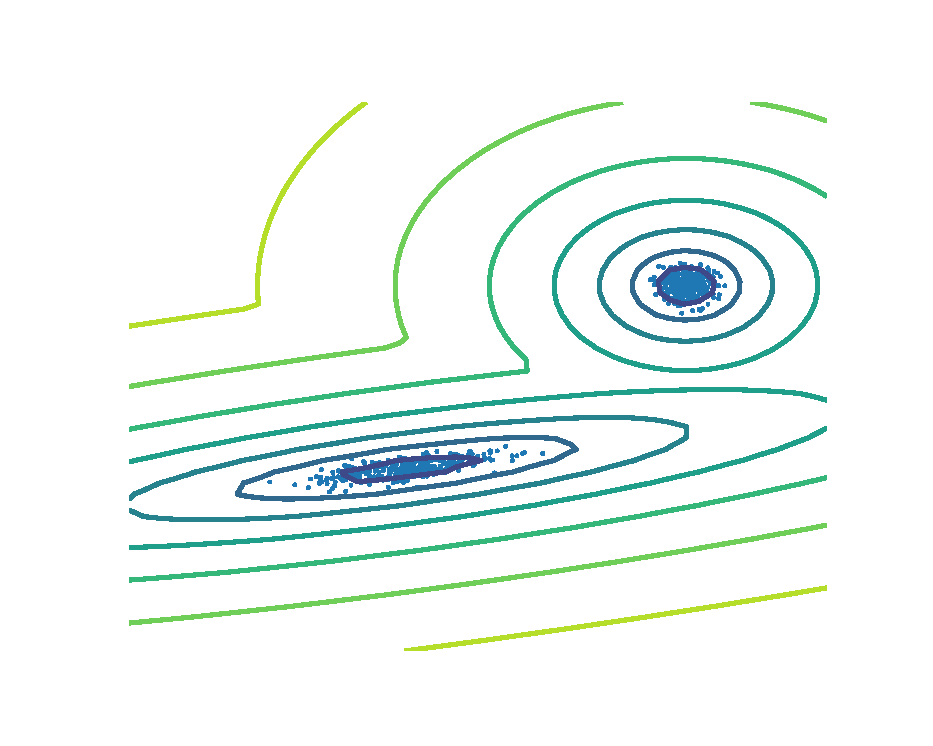
\includegraphics[width=0.33\textwidth]{figs/gmm.eps}
			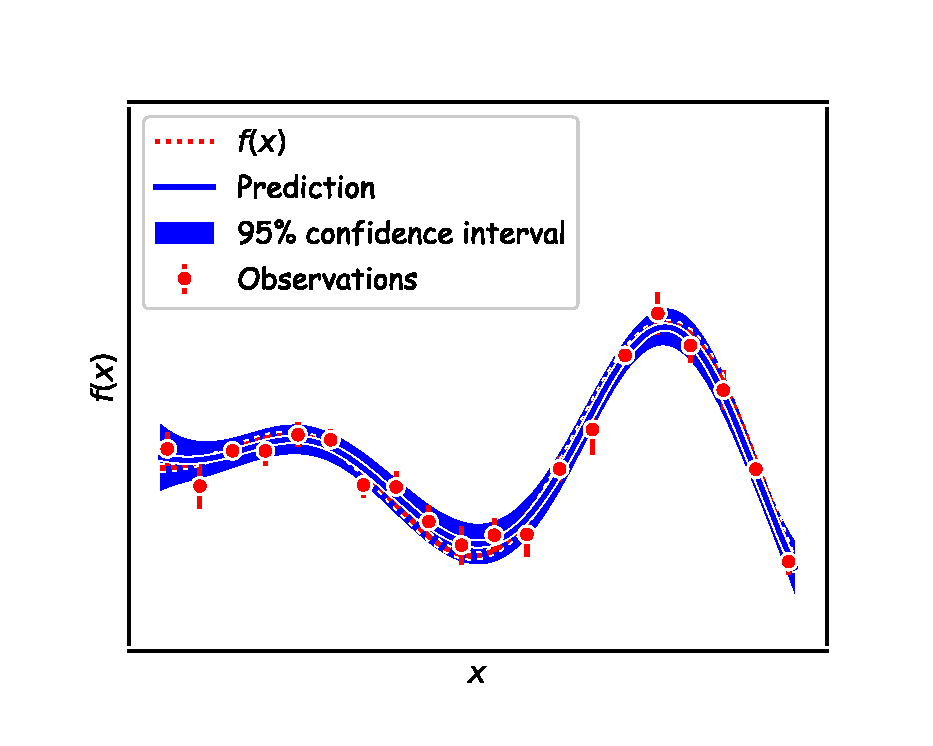
\includegraphics[width=0.33\textwidth]{figs/gp.eps}
		\end{center}
	\end{figure}
	\begin{center}
		$\pi(x, \theta)$~(joint probability) 
	\end{center}
	\begin{itemize}		
		\item $\blacktriangleright$ 
		Update beliefs about model parameters given data\\
		$\bm{\pi(\theta|x)} = \frac{\color{blue!50!green}{\overbrace{\pi(x|\theta)}^{\text{\clap{\textcolor{blue!50!green}{data likelihood~}}}}} \color{blue!70!red}{\overbrace{\pi(\theta)}^{\text{\textcolor{blue!70!red}{\clap{~prior}}}}}}{\color{blue}{\underbrace{\pi(x)}_{\text{\clap{\textcolor{blue}{evidence}}}}}}$~(Bayes' theorem)
		\item $\blacktriangleright$
		Compute predictive probabilities on unseen data
		$ \pi(x^\star| x) = \int \pi(x^\star |\theta)\color{black}{\bm{\pi(\theta|x)}} d\theta \approx \frac{1}{S} \sum_{s=1}^{S} \pi(x^\star|\theta_s)$, 
		$\theta_s \sim \pi(\theta|x)$, for $s=1\ldots S$
	\end{itemize}
\end{frame}


\begin{frame}
	\frametitle{Large Scale Inference}
	\begin{itemize}
		\item  $\circ$ Update beliefs given \textbf{massive-scale} data 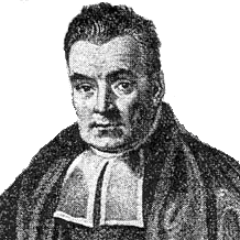
\includegraphics[width=2cm,height=2cm]{figs/Bayes.png} \hfill $\pi(\theta|x) = \frac{1}{Z} \pi(x|\theta) \pi(\theta)$ \hfill \textcolor{darkred}{Hard to compute!}
		\item  $\circ$ \textbf{Intuition:} For parametric models there is lot of \texbf{redundancy}---\textbf{\emph{compress the dataset}} into a summary and run inference thereon
	\end{itemize}
	\begin{figure}{\textwidth}
		\centering
		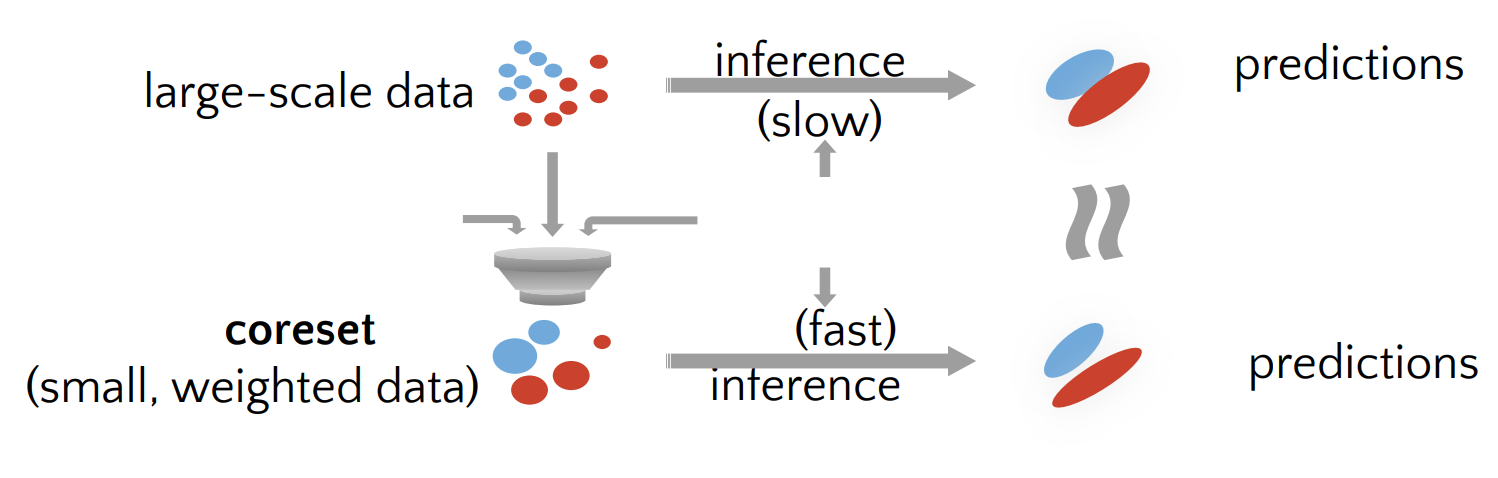
\includegraphics[width=7cm]{figs/coresets_high_level.png}
		\label{fig:coresets_high_level}
	\end{figure}
\end{frame}


\begin{frame}
	\frametitle{Problem Statement}
	\begin{tcolorbox}[colback=gray!5,colframe=white!40!black]  
		\centering
		\textbf{In modern ML, datasets scale outpaces our ability to process them}
	\end{tcolorbox}
	\textbf{Proposal: Replace datasets with \emph{coresets}} 
	\begin{itemize}
		\item $\blacktriangleright$ \texbf{\emph{scale up}} expensive inference methods
		\item $\blacktriangleright$ good \texbf{\emph{quality monitoring/statistical guarantees}}
		\item  $\blacktriangleright$ high degree of \texbf{\emph{automation}}, black-box inference
		\item $\blacktriangleright$ \texbf{\emph{general purpose}} Bayesian inference, for
	 \emph{conditionally independent data}, \emph{tractable likelihood functions} 
		\item  $\blacktriangleright$ \textbf{overall} good statistical/computational trade-off \emph{under statistical privacy and robustness constraints}
	\end{itemize}
\end{frame}

\begin{frame}
	\frametitle{Bayesian coresets at a glance: From importance sampling to variational inference}
	\begin{align*}
	\mcL(w, \theta):=\sum_{n=1}^{N} w_n \mcL_n(\theta), \;\;\text{s.t.}\;\; |\mcL(w, \theta) - \mcL(\theta)| \leq \eps |\mcL(\theta)|, \;\;\forall \theta \in \Theta
	\end{align*}
	$\blacktriangleright$ Principles of subset selection
	\begin{itemize}
		\item $\circ$ \textbf{Importance sampling} using \emph{sensitivity} $\sigma_n := \underset{\theta \in \Theta}{\sup}\big|\frac{\mcL_n(\theta)}{\mcL(\theta)}\big|$~\citep{huggins16}
		\item $\circ$ \textbf{Sparse regression} using \emph{inner product norms} $ \big\langle \mcL - \mcL(w), \mcL_n \big\rangle_\mcH$~\citep{campbell19jmlr}
		\item $\circ$ \textbf{Sparse variational inference} using the \emph{KL divergence} ~\citep{campbell19neurips}
	\end{itemize}
\end{frame}	

\begin{frame}
		\frametitle{Privacy}
		\begin{figure}
			\centering 
			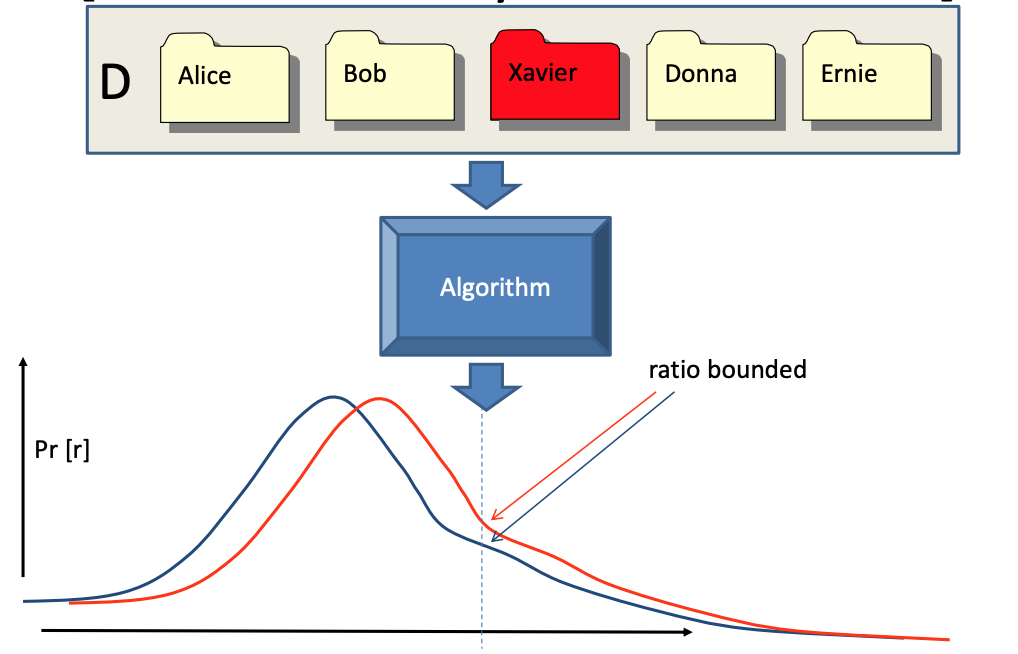
\includegraphics[width=5cm,height=4cm]{figs/dp.png}
			\caption{Differential Privacy (DP) visually \emph{(\textsuperscript{\textcopyright}Aaron Roth)}}
		\end{figure}
	\textbf{Approximate DP}: A randomized mechanism $\mcM : X \rightarrow Y$ is $(\veps, \delta)$-DP if for \emph{\textbf{all}} neighbouring inputs $x, x': x \approx x'$ and \emph{\textbf{all}} sets of outputs $E \subseteq Y$ we have 
	$P[\mcM(x) \in E] \leq e^\veps P[\mcM(x') \in E] + \delta$
\end{frame}


\begin{frame}
	\frametitle{Robustness}
	Huber's $\eps$-contamination model
	\begin{columns}
		\begin{column}{.39\textwidth}
			\hfill 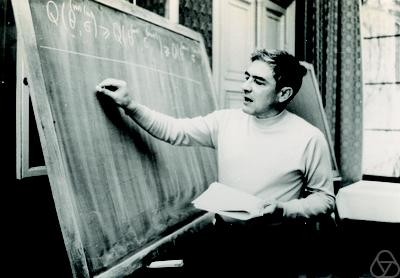
\includegraphics[width=1.\textwidth]{figs/Huber.jpg}\\ 
		\end{column}
		\begin{column}{.69\textwidth}
			\hfill 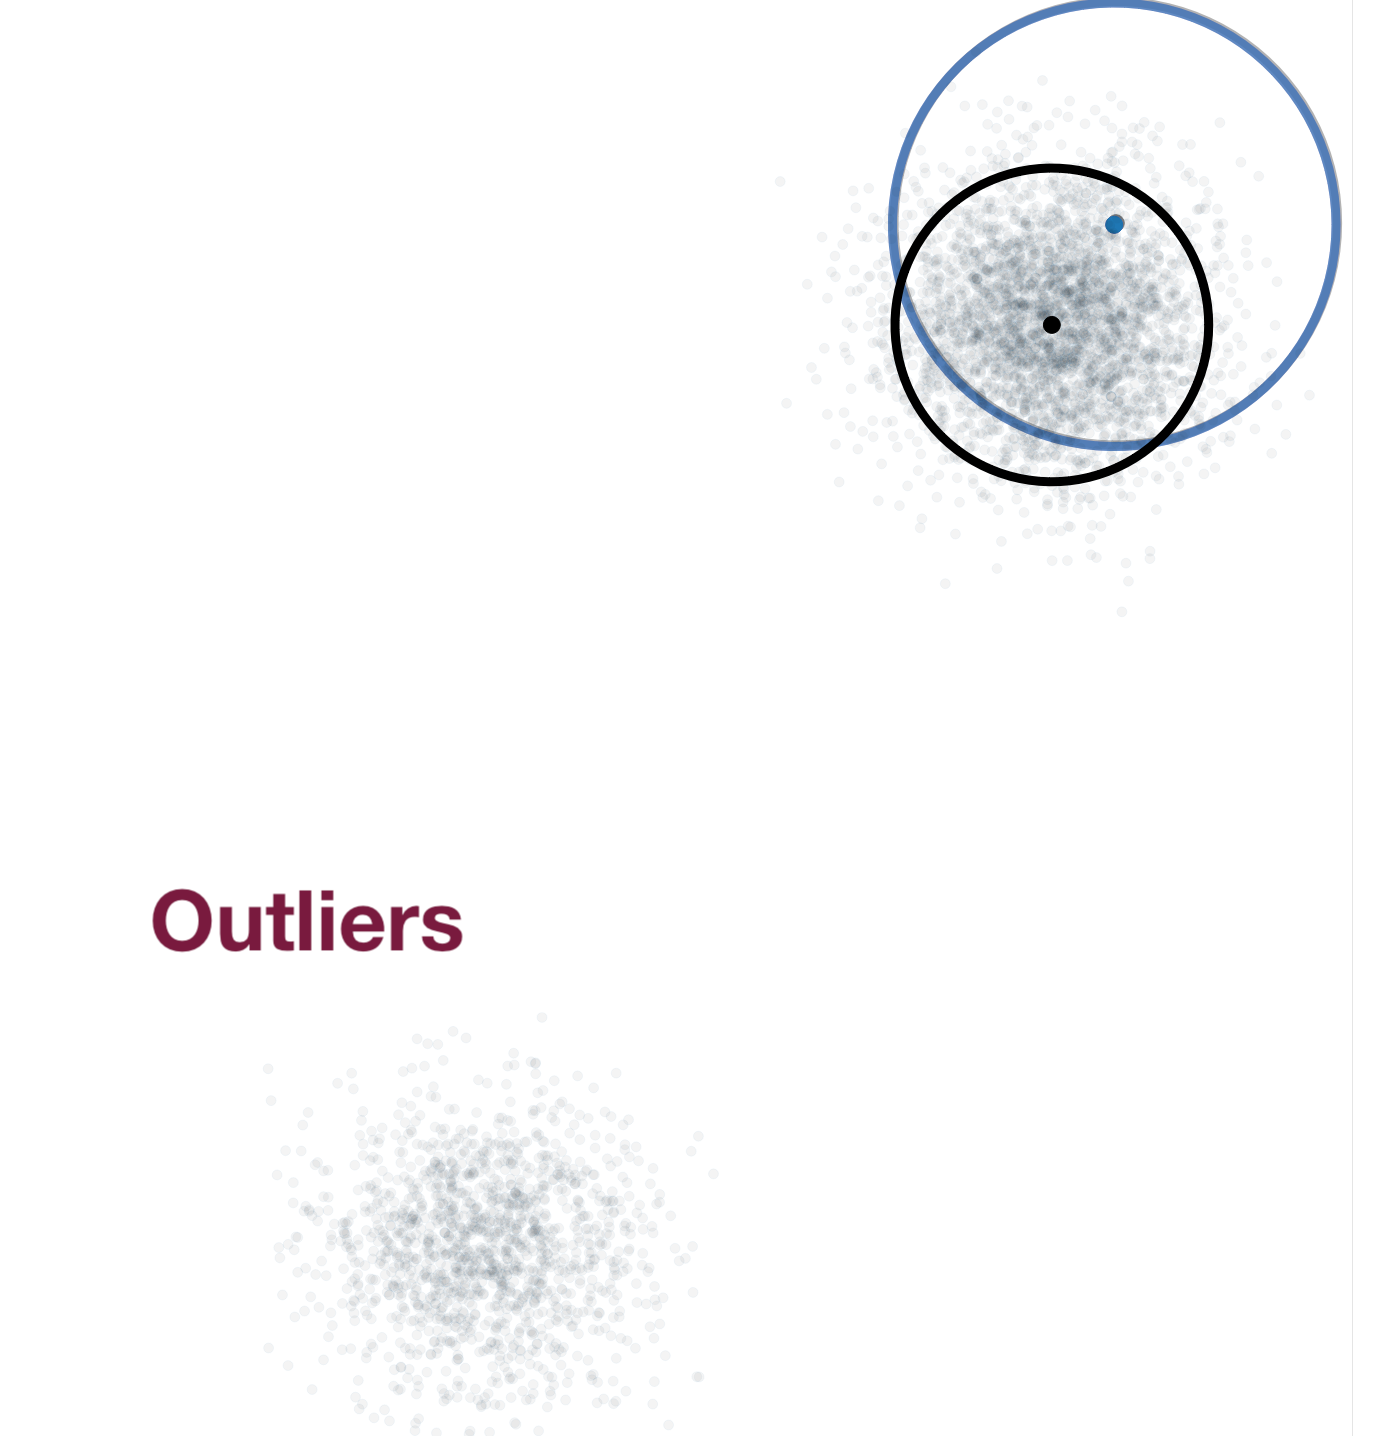
\includegraphics[width=.5\textwidth]{figs/contaminated-gaussian.png}\\ 
		\end{column}
	\end{columns}
	\definecolor{darkred}{rgb}{0.55, 0.0, 0.0}
	$(x_n)_{n=1}^{N}\sim G_{\eps, q}:= (1-\eps)\cdot \pi + \eps \cdot \color{darkred}{q}$~\citep{huber92},
	where
	\\  $\circ$ $\eps \in (0,1)$, 
	\\  $\circ$ $\pi$ follows our statistical assumptions, and 
	\\  $\circ$ $\color{darkred}{q}$ is an arbitrary distribution of outliers
\end{frame}


\begin{frame}
	\frametitle{Robustness}
	\begin{columns}
		\begin{column}{0.48\textwidth}
			\centering 
			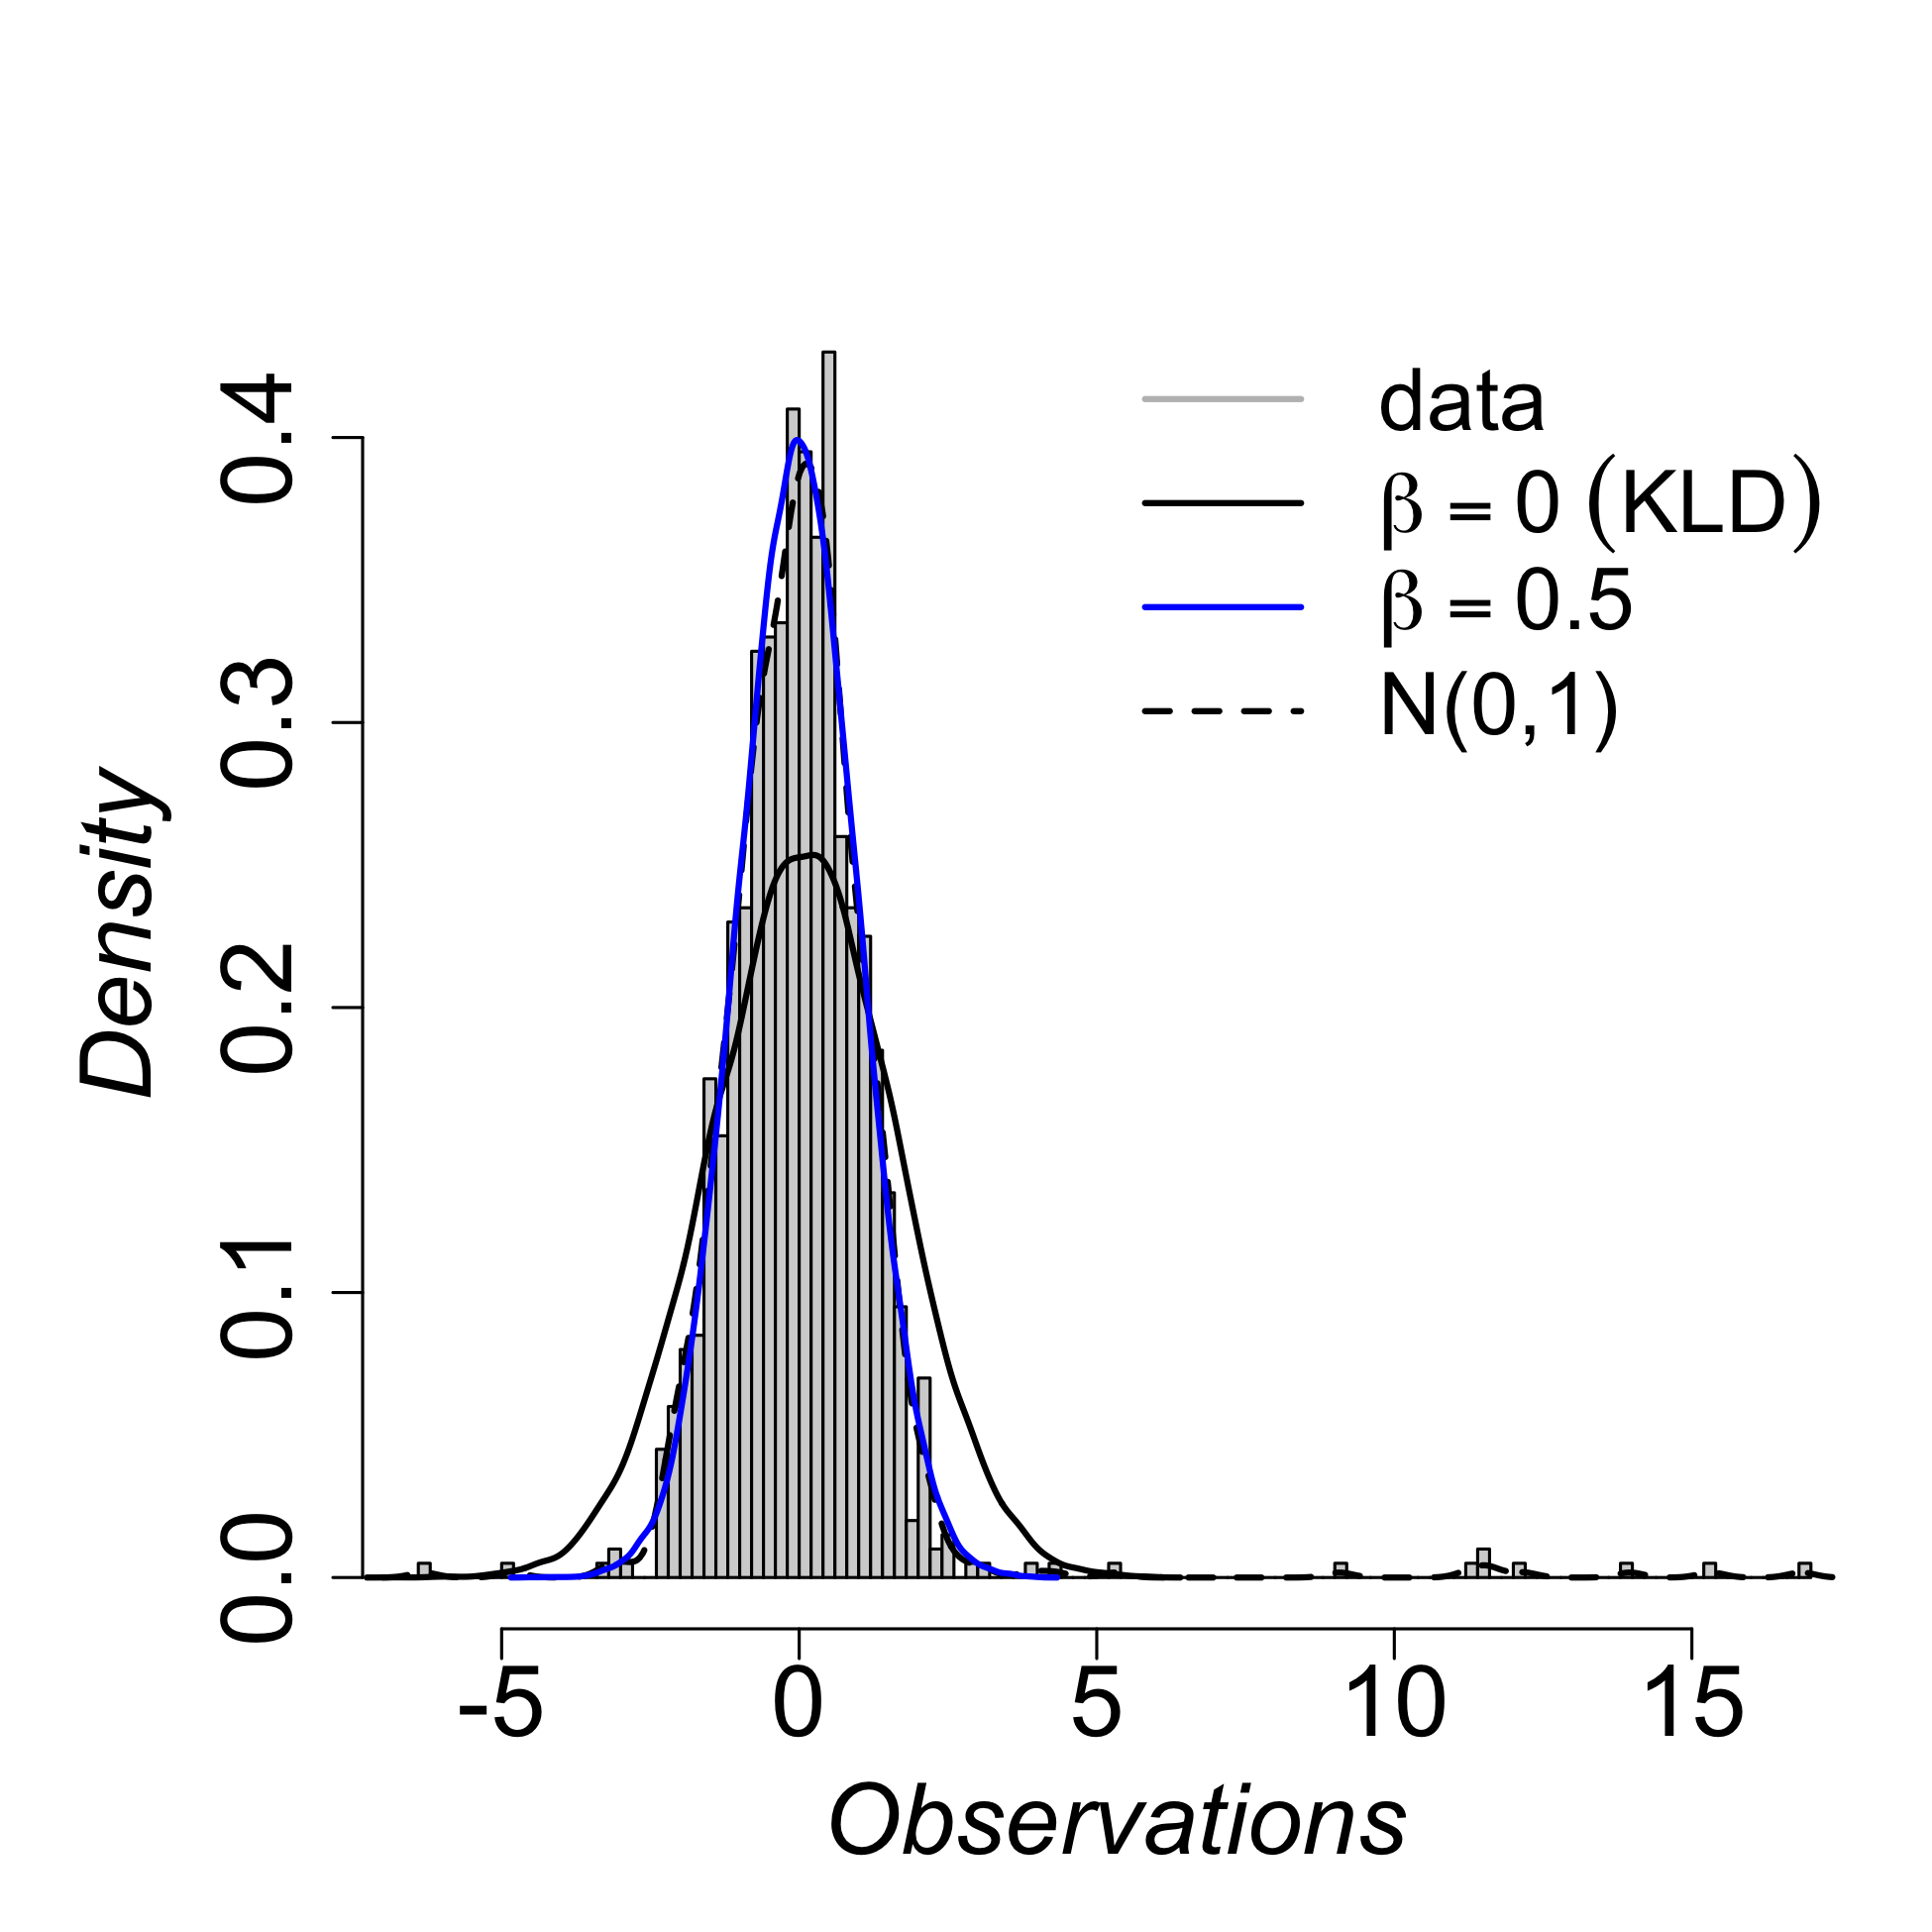
\includegraphics[width=3.6cm,height=3.4cm]{figs/density.png}%
		\end{column}
		\begin{column}{0.48\textwidth}
			\centering
			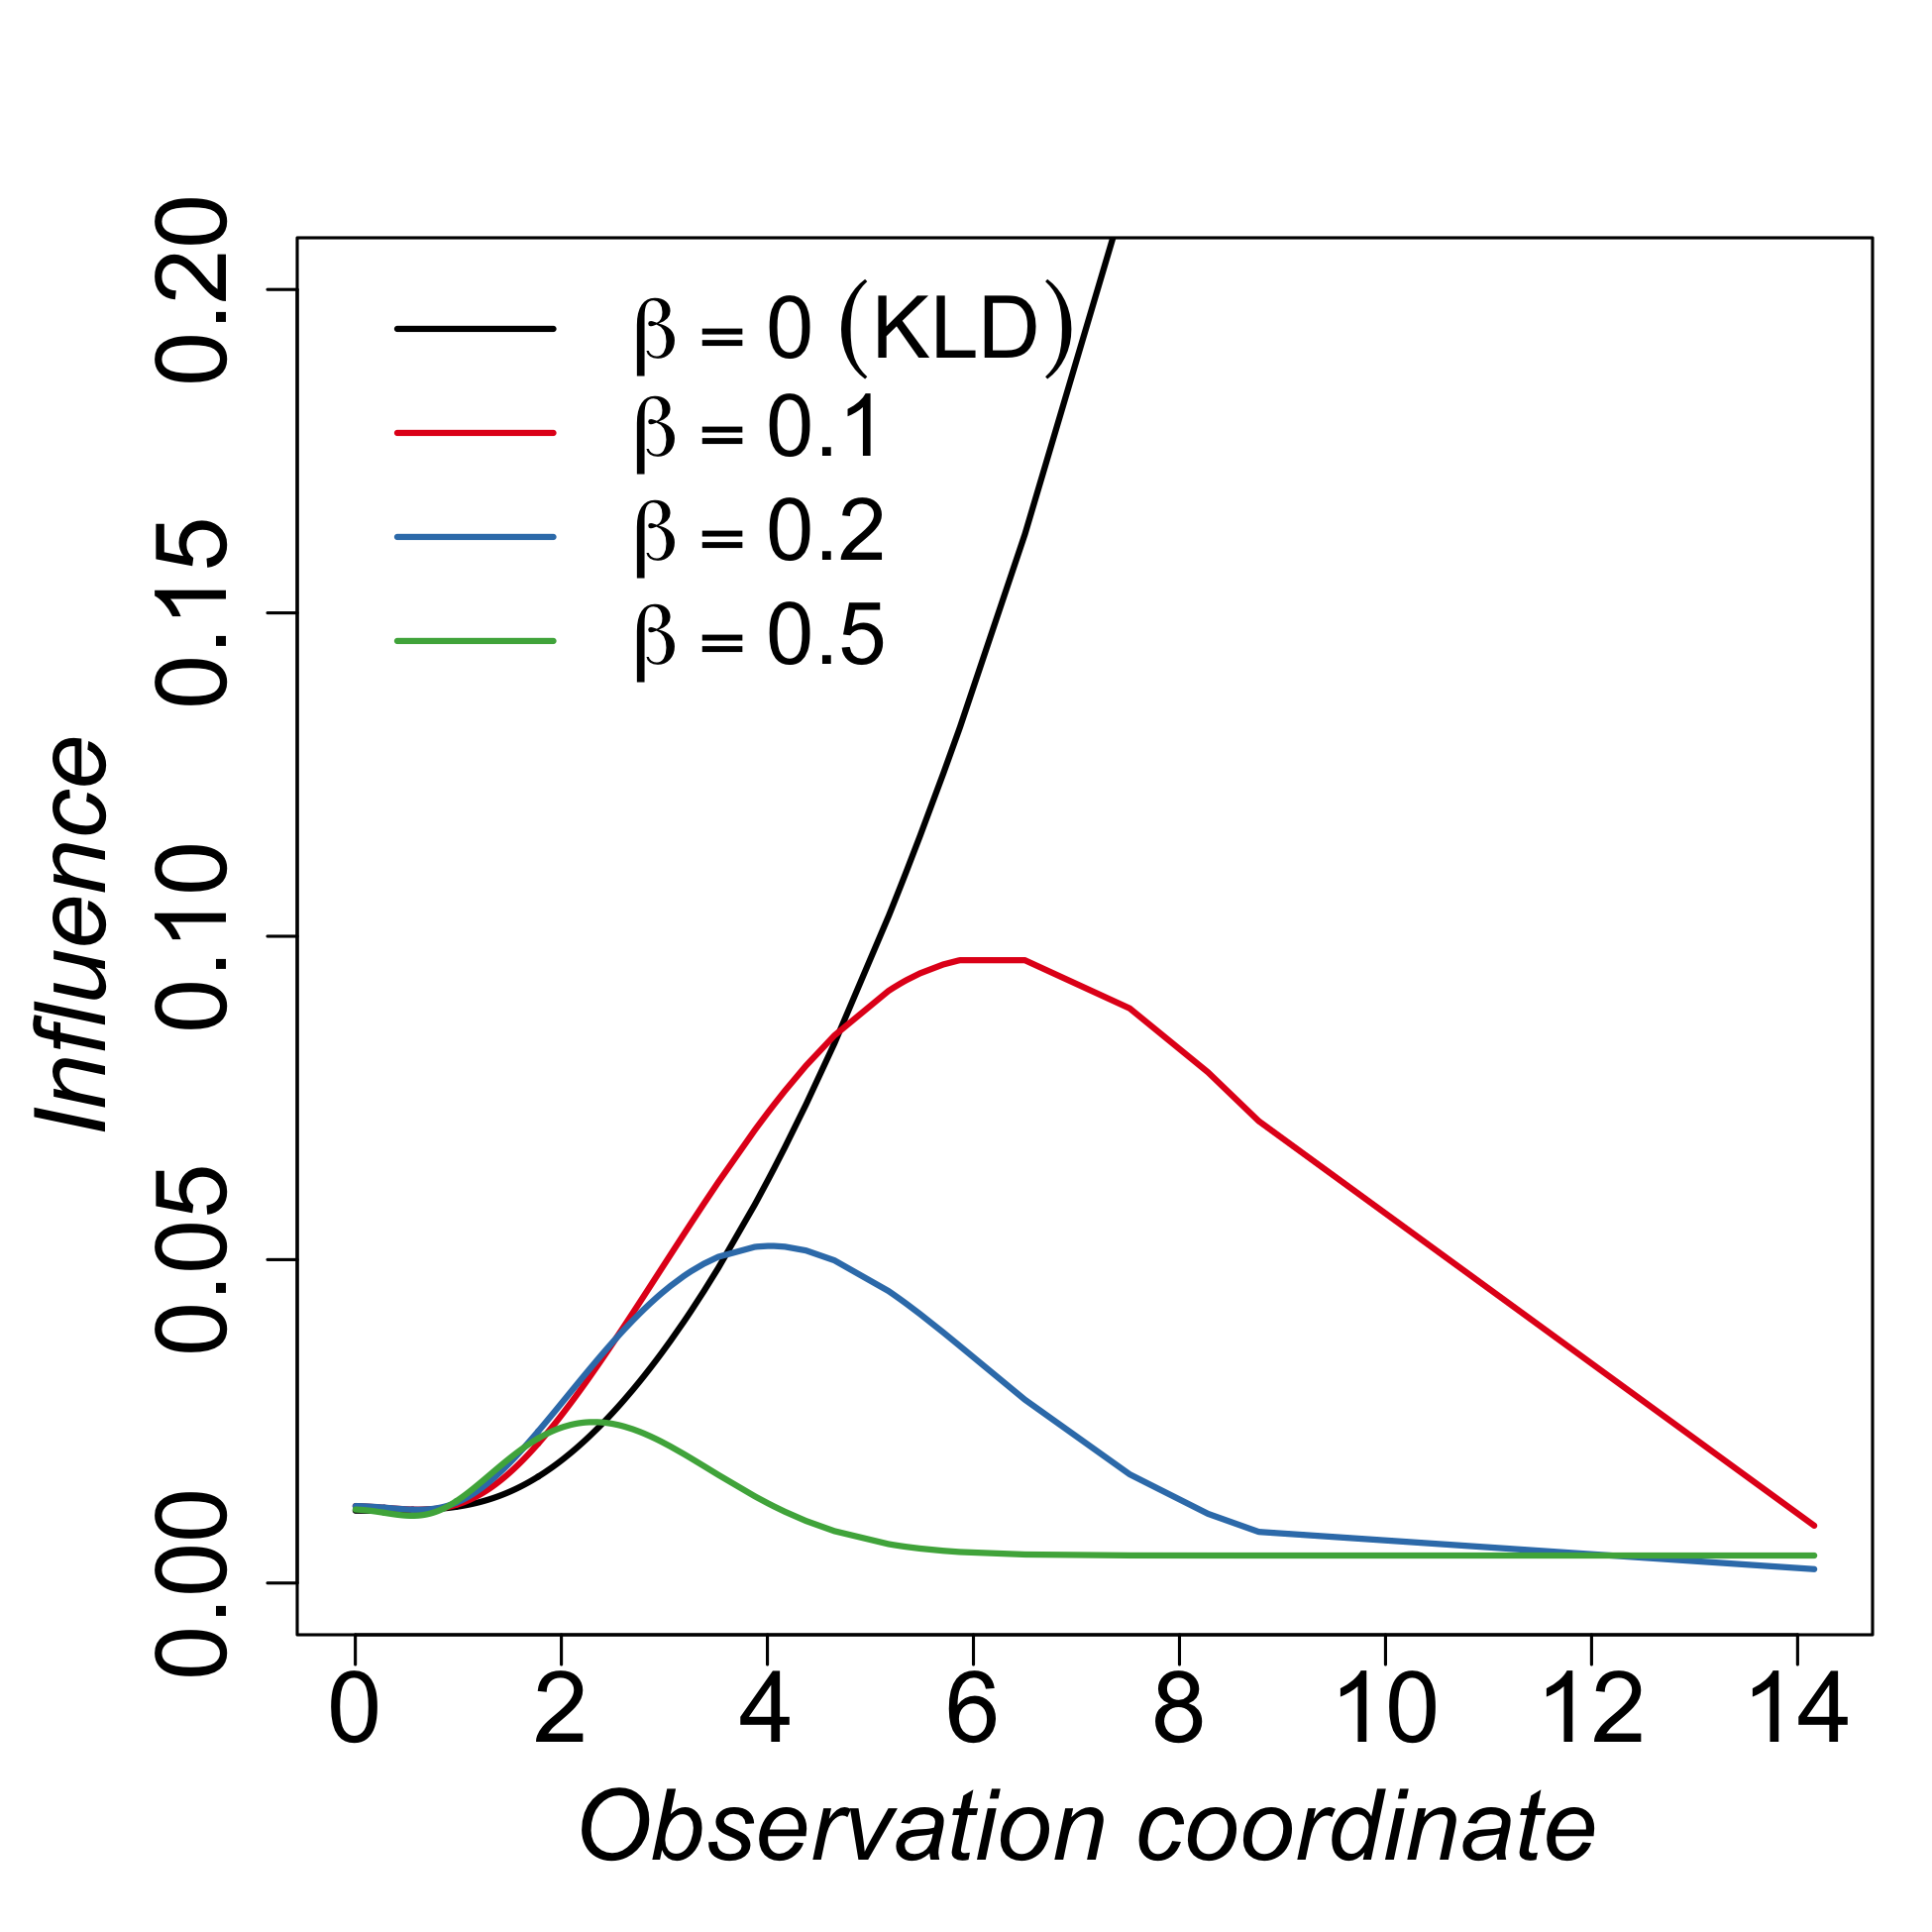
\includegraphics[width=3.6cm,height=3.4cm]{figs/influence.png}%
		\end{column}
	\end{columns}
		\begin{itemize}
			\item $\blacktriangleright$ \textbf{Influence functions}: $IF(q, T, G) = \frac{\partial}{\partial \eps} T(G_{\eps, q}(x))\Bigg\rvert_{\eps=0}$ \citep{huber09}.
			\item $\blacktriangleright$ \textbf{Bayesian sensitivity}: metric between posteriors conditioned on neighboring datasets, e.g. $D_{FR}(\{x_i\}) \leftarrow \text{distance}(\pi(\theta|x)||\pi(\theta|x\cup\{x_i\}))$\citep{kurtek15}.	
		\end{itemize}
\end{frame}


\begin{frame}{Structure}
	\begin{itemize}
		\item[I.]\textbf{Bayesian Pseudocoresets} \small{\citep{psvi}} \\
		A variational framework for scalable Bayesian inference, that achieves superior summarization quality in high-dimensions and admits differentially private constructions
		\item[II.]\textbf{$\beta$-Cores} \small{\citep{beta-cores}}  \\
		A framework for Bayesian summarization designed for observations following the Huber contamination model.
	\end{itemize}
\end{frame}


%%%%%%%%%%%%%%%%%%%%%%%%%%%%%%%%%%%%%%%%%%%%%%%%%%%%%%%
%%%%%%%%%%%%%%%%%%%%%%%%%%%%%%%%%%%%%%%%%%%%%%%%%%%%%%%

%%%%%%%%%%%%%%%%%%%%%%%%%%%%%%%%%%%%%%%%%%%%%%%%%%%%%%%
%%%%%%%%%%%%%%%%%%%%%%%%%%%%%%%%%%%%%%%%%%%%%%%%%%%%%%%
%% NEURIPS
%%%%%%%%%%%%%%%%%%%%%%%%%%%%%%%%%%%%%%%%%%%%%%%%%%%%%%%
%%%%%%%%%%%%%%%%%%%%%%%%%%%%%%%%%%%%%%%%%%%%%%%%%%%%%%%

\begin{frame}
	\LARGE{\textbf{I. Bayesian Pseudocoresets}}
\end{frame}



\begin{frame}
	\frametitle{Bayesian Coresets}
	$\circ$ \textbf{Riemannian Coresets}~\citep{campbell19neurips}
	\begin{figure}
		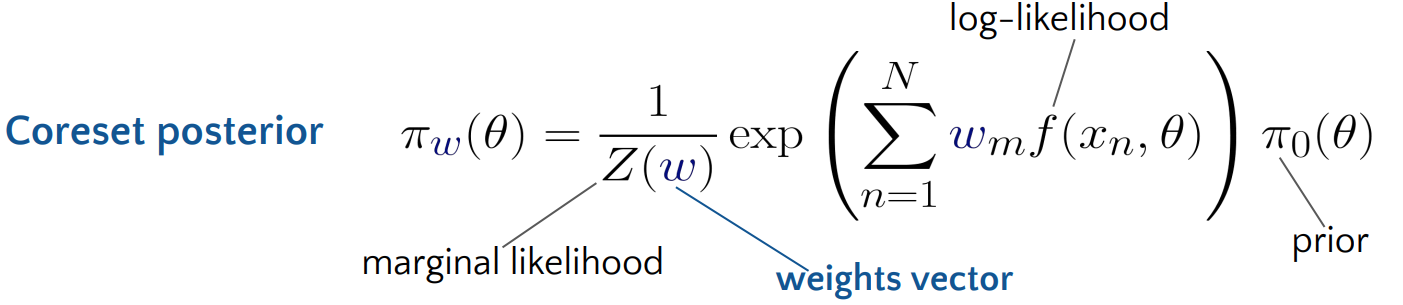
\includegraphics[width=1.\linewidth]{figs/sparsevi_posterior.png}
	\end{figure}
	$\circ$ \textbf{Sparse Variational Inference}
	\begin{align*}
	 w^\star = \argmin_{w\in\reals^N} \kl{\pi_w}{\pi}\label{eq:coresets-vi} \quad \quad
	\text{s.t.} \quad w \geq 0, \; \|w\|_0 \leq M
	\end{align*}
\end{frame}

\begin{frame}
	\frametitle{Limitation I: High-dimensional data}
	\begin{tcolorbox}[colback=grey!5,colframe=white!40!black,title=KL lower bound in Gaussian mean inference via coresets]  
		\begin{itemize}
		\item $\circ$ Data $(X_n)_{n=1}^N \distiid \distNorm(0, I)$ in $\reals^d$, prior
		$\mu \dist \distNorm(0, I)$, likelihood
		$(X_n)_{n=1}^N  \distiid \distNorm(\mu, I)$
		\item  $\circ$ Coreset size $ M $, \emph{optimal} coreset posterior $\pi_{w^\star}$ 
		\item $\blacktriangleright$ Then $\forall M<d$ with high probability
		\begin{align*}
		\kl{\pi_{w^\star}}{\pi} \geq \frac{1}{2}\frac{N-M}{1+N} F(d-M, M, N)
		\end{align*}
		(RHS visualized in next slide)
		\end{itemize}
	\end{tcolorbox}
\end{frame}


\begin{frame}
	\frametitle{Limitation I: High-dimensional data}
			\centering
	\begin{figure*}
		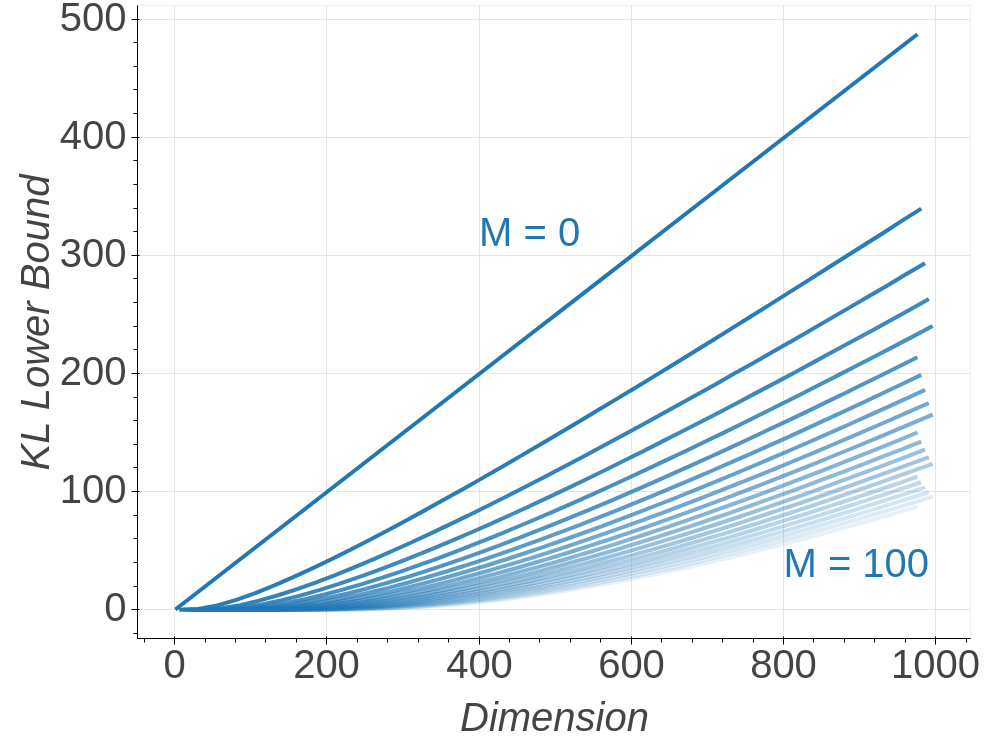
\includegraphics[width=.8\linewidth]{figs/klbound.png}
	\end{figure*}
\end{frame}

\begin{frame}
	\frametitle{Limitation I: High-dimensional data}
	$\circ$ In Gaussian mean inference coreset covariance and mean are 
	\begin{align*}
	\Sigma_w &=\left(1+\sum_{n=1}^N w_n\right)^{-1} I, & \mu_w &= \Sigma_w \sum_{n=1}^N w_n X_n.\label{eq:gausswpost}
	\end{align*}
	
	which can be replicated via \emph{a point}
	\begin{align*}
	& U = \left(\sum_{n=1}^Nw_n\right)^{-1}\sum_{n=1}^N w_nX_n
	& \text{with weight}\;\; \sum_{n=1}^N w_n.
	\end{align*}
	$\circ$ True posterior can be exactly computed via a \textbf{\emph{single pseudopoint}}
	\begin{align*}
	& U = \frac{1}{N}\sum_{n=1}^N X_n & \text{with weight}\;\; N.
	\end{align*}
\end{frame}

\begin{frame}
	\frametitle{Limitation II: Privacy}
	\begin{itemize}
		\item $\circ$	Existing constructions are incompatible with formal privacy definitions, as subset
		of datapoints gets revealed 
		\item $\circ$	For sensitive datasets, summarization
		should use synthetic data
		\begin{figure*}
			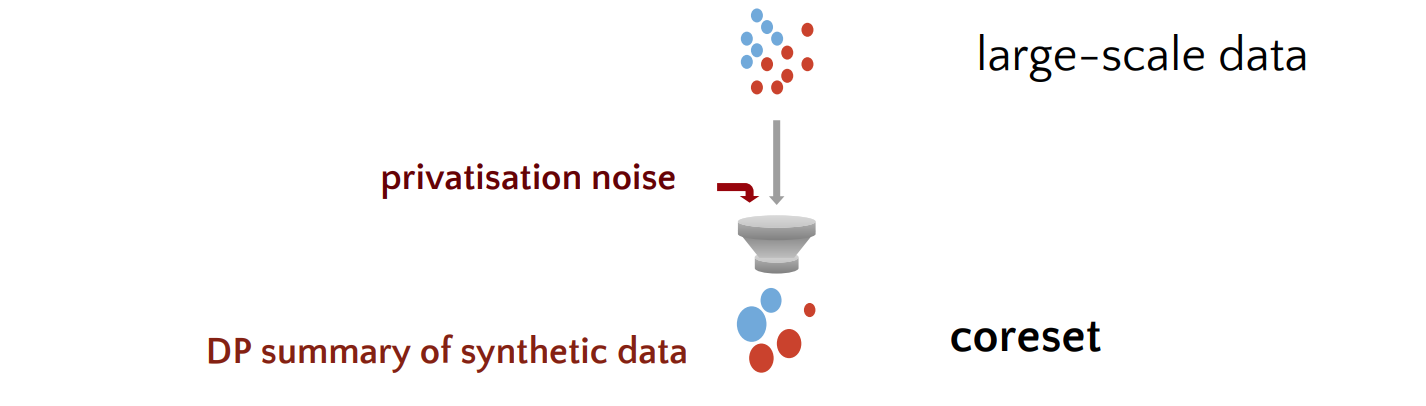
\includegraphics[width=1\linewidth]{figs/dp_summarize.png}
		\end{figure*}
	\end{itemize}
\end{frame}

\begin{frame}
	\frametitle{Applications of summarization: (Pseudo)data as \emph{"approximate sufficient statistics"}}
	\begin{itemize}
		\item For scalability
		\begin{itemize}
			\item $\blacktriangleright$ Linear regression, clustering, herding, priors for DGMs~\citep{bachem15,bachem17}
			\item $\blacktriangleright$ Nystr\"{o}m method, leverage scores for computing with kernels~\citep{drineas05,musco17,agrawal19},
			\item $\blacktriangleright$ Inducing (pseudo-)input methods in Gaussian processes~\citep{snelson05,titsias09,bauer16}
		\end{itemize}
		\item For privacy
		\begin{itemize}
				\item $\blacktriangleright$ Kernel mean embeddings, sparse regression~\citep{zhou08,balog18}
		\end{itemize}
	\end{itemize}
\end{frame}

\begin{frame}
	\frametitle{Bayesian Pseudocoresets}
		\begin{itemize}
		\item  $\blacktriangleright$ Pseudocoreset posterior
	\begin{align*}
		\pi_{u,w}(\theta) = \frac{1}{Z(u, w)} \exp \left( \sum_{m=1}^{M} w_m f(u_m,\theta) \right) \pi_0(\theta)
	\end{align*}
	where $(u_m)_{m=1}^{M}$ are \textbf{learnable pseudodata points}.
		\item  $\blacktriangleright$ Variational inference over \textbf{pseudodata locations} and \texbf{weights}
	\begin{align*}
	u^\star, w^\star = \argmin_{\substack{u\in\reals^{d \times M}}, w\in\reals^M_+}\,\, \kl{\pi_{u,w}}{\pi}. 
	\end{align*}
		\end{itemize}
\end{frame}


\begin{frame}
	\frametitle{Pseudocoresets Construction}
	\begin{align*}
	u^\star, w^\star = \argmin_{\substack{u\in\reals^{d \times M}}, w\in\reals^M_+}\,\, \kl{\pi_{u,w}}{\pi}. 
	\end{align*}	
	 $\circ$ Gradients \wrt variational parameters are tractable 
	\begin{align*}
	\nabla_{u_m}\mathrm{D}_{\mathrm{KL}} = -w_m\cov_{u,w}\left[(\nabla_u f)(u_m), f(x, \theta)^T1 - f(u, \theta)^Tw\right]
	\end{align*}
	\begin{align*}
	 \nabla_w\mathrm{D}_{\mathrm{KL}} = - \cov_{u,w}[f(u, \theta) ,f(x, \theta)^T1 - f(u, \theta)^Tw]
	\end{align*}
\end{frame}


\begin{frame}
	\frametitle{Black-box Batch  Pseudocoreset Construction}
	\vspace{-0.5cm}
	\begin{itemize}
		\item $\blacktriangleright$ Pseudocode sketch
		\scriptsize 
		\begin{tcolorbox}
			\begin{algorithmic}[1]
				\Procedure{PSVI}{ likelihood function $f$, data $x$, prior $\pi_0$, coreset size $M$, minibatch size $B$, $\#$ of optimization steps $T$, $\#$ of samples from coreset iterates $S$, learning rate schedule $(\gamma_t)_{t=0}^{\infty}$}
				\LineCommentIndent{\textbf{Initialize} using a uniformly chosen subset of the full dataset}
				\For{$ t = 1, \ldots, T$} 
					\LineCommentIndent{\mbox{Take $S$ samples from current pseudocoreset posterior}}\\
					\LineCommentIndent{\mbox{Get a minibatch of $B$ points from the full dataset}} 
						\For{$s = 1, \dots, S$} 	
							\LineCommentIndent{\mbox{Compute (gradient) log-likelihood discretizations}}\\
						\EndFor
					\LineCommentIndent{\mbox{Take steps using MC \textbf{gradients for $w$ and $u$}}}
				\EndFor
				\State\Return $w$, $u$%, $\beta$
				\EndProcedure		 
			\end{algorithmic}
		\end{tcolorbox}
		\normalsize
	\end{itemize}
\end{frame}

\begin{frame}
	\frametitle{Differentially Private Construction of Bayesian Pseudocoreset}
	\vspace{-4pt}
	\begin{columns}
		\begin{column}[t]{0.4\textwidth}
		\begin{itemize}
			\item $\blacktriangleright$ \textbf{Initialize}  from the statistical model
			\item $\blacktriangleright$ \textbf{Iterate} Compute private gradients via applications of the \textbf{subsampled Gaussian mechanism}~\citep{abadi16}
		\end{itemize}
		\end{column}
	\pause
		\begin{column}[t]{0.6\textwidth}
		\begin{itemize}
			\item --- {Moments accountant}
			\item --- {No extra  cost when sampling from the coreset}
			\item --- {No global sensitivity computation}
			\item --- {Adaptive gradient clipping} 
			\item --- {Constructed private pseudocoresets can be queried \emph{ad infinitum}} 
		\end{itemize}
		\end{column}
	\end{columns}
\end{frame}

\begin{frame}
	\frametitle{Experiments I~(High-dimensional Gaussian mean inference)}
	\centering 
	$\circ$ 500 dimensions, 1K datapoints\\
	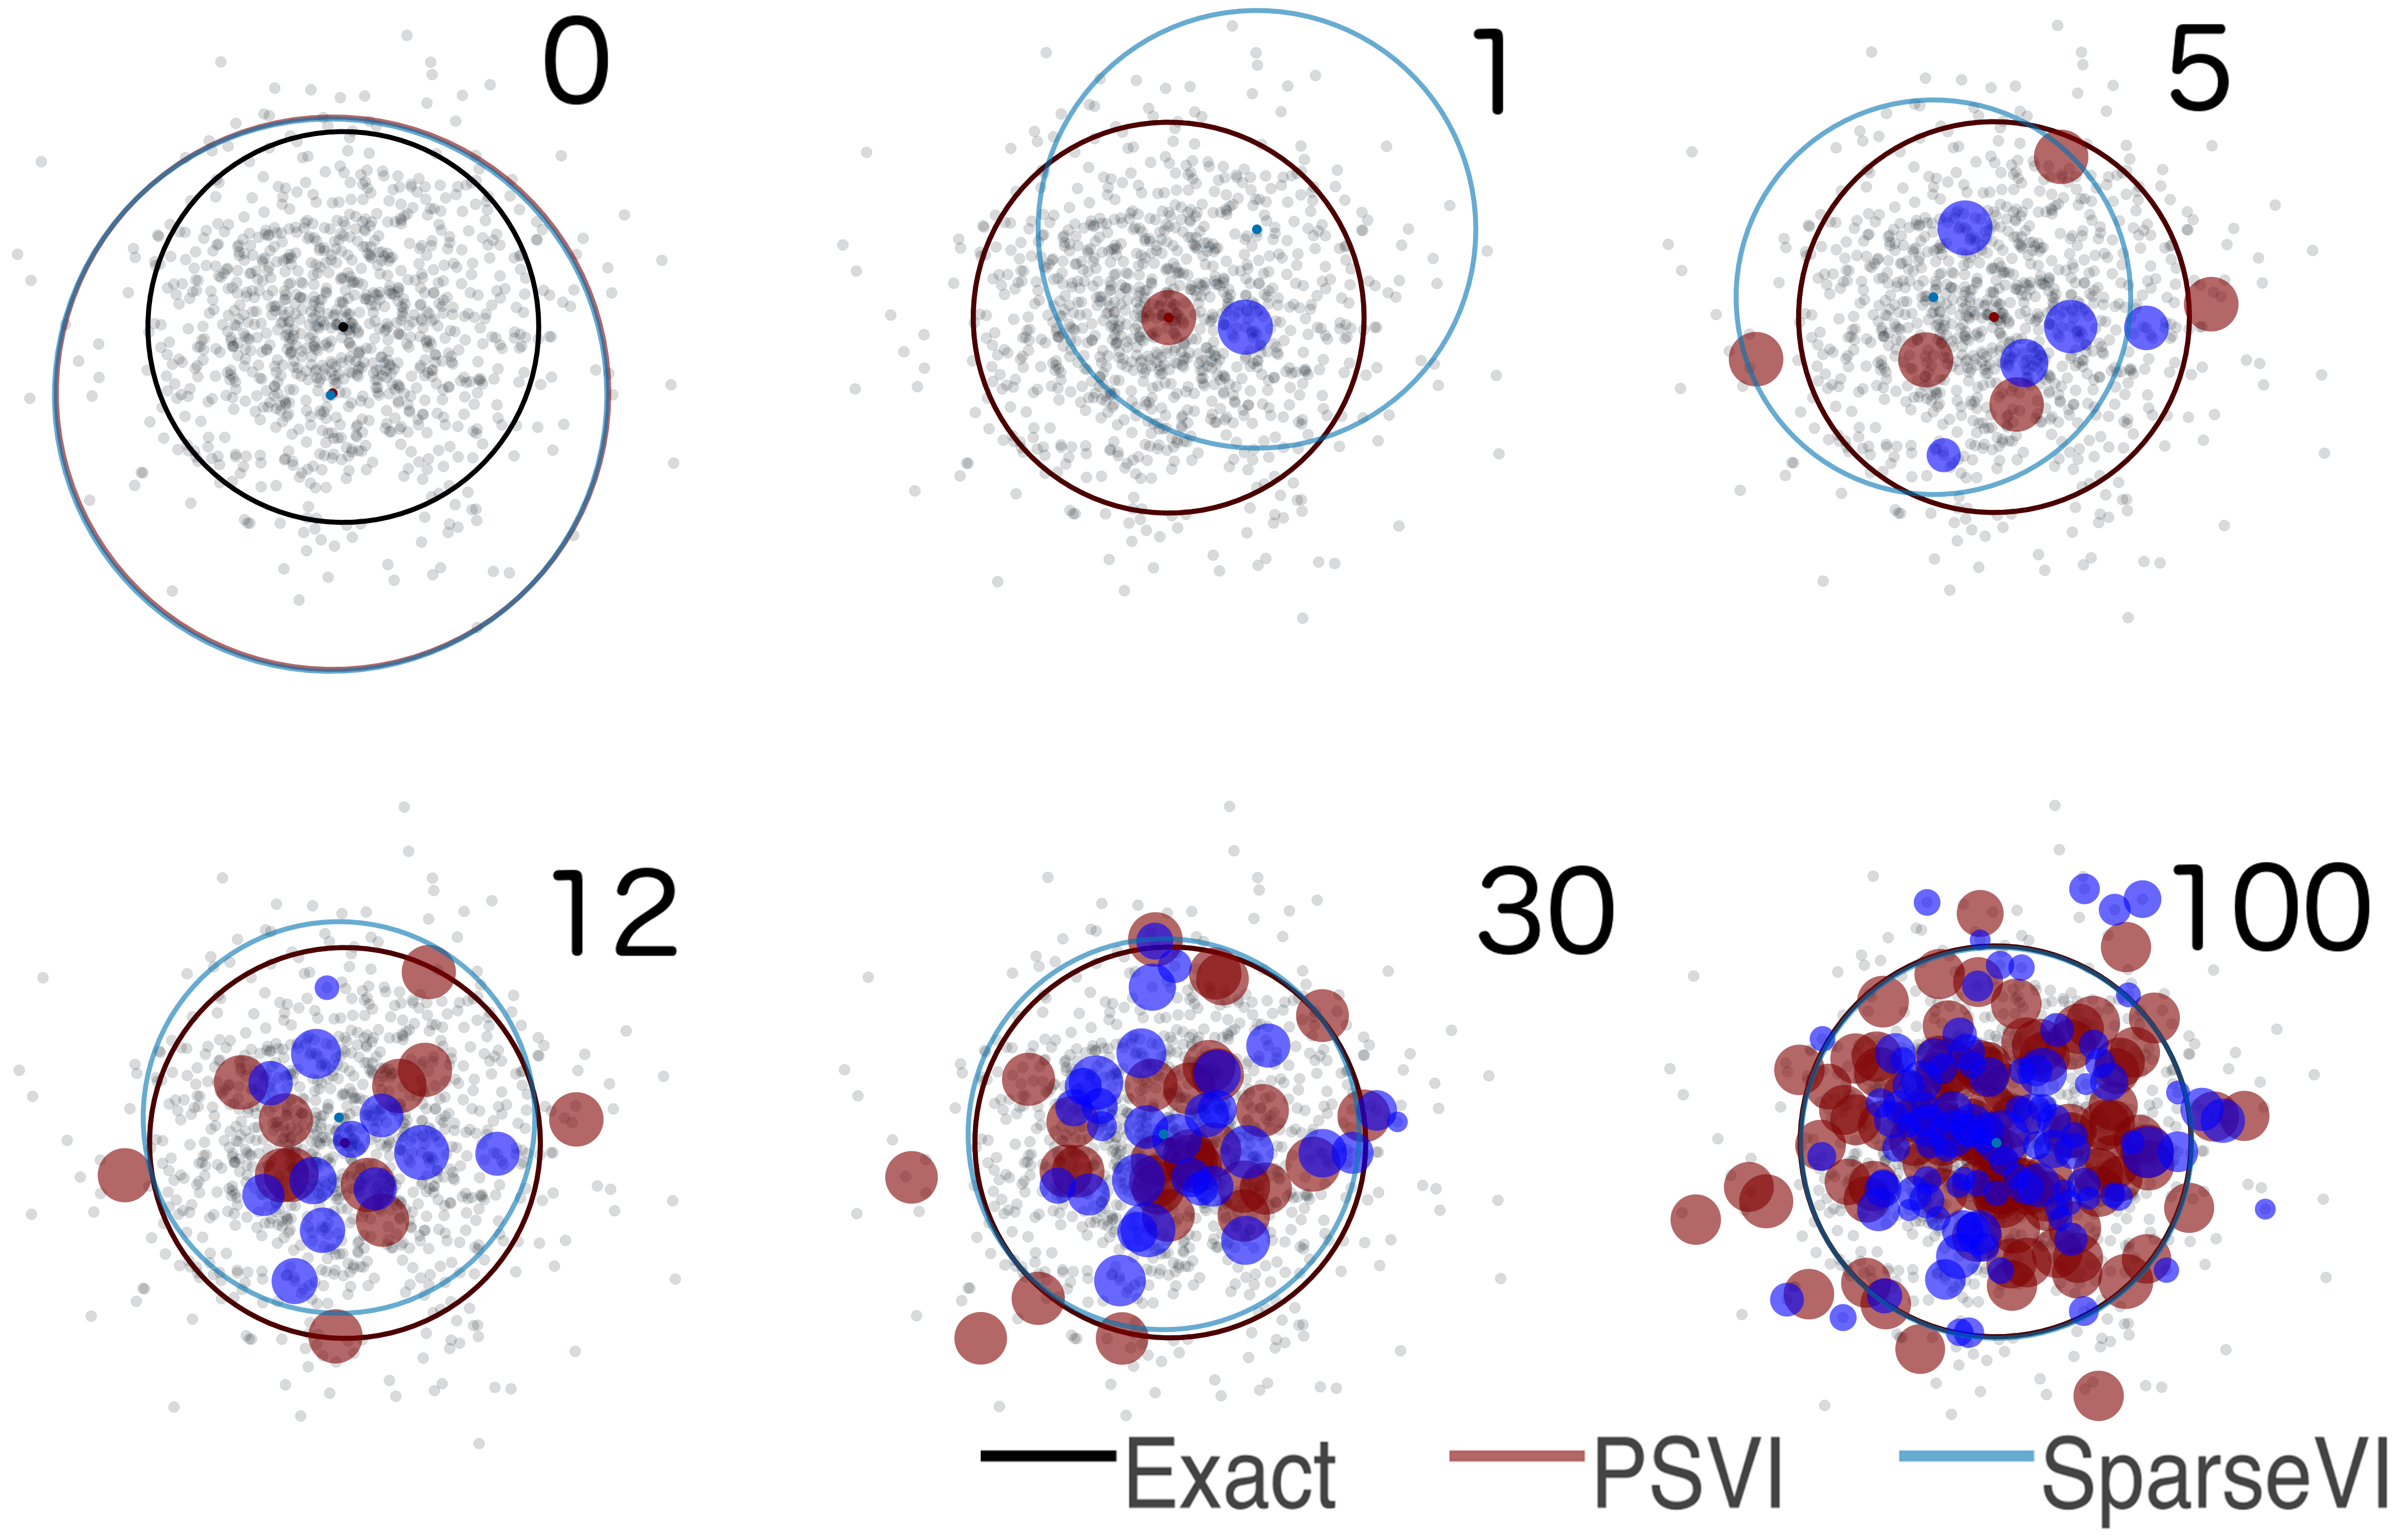
\includegraphics[width=.49\textwidth]{figs/d500_pts_combined.png}
	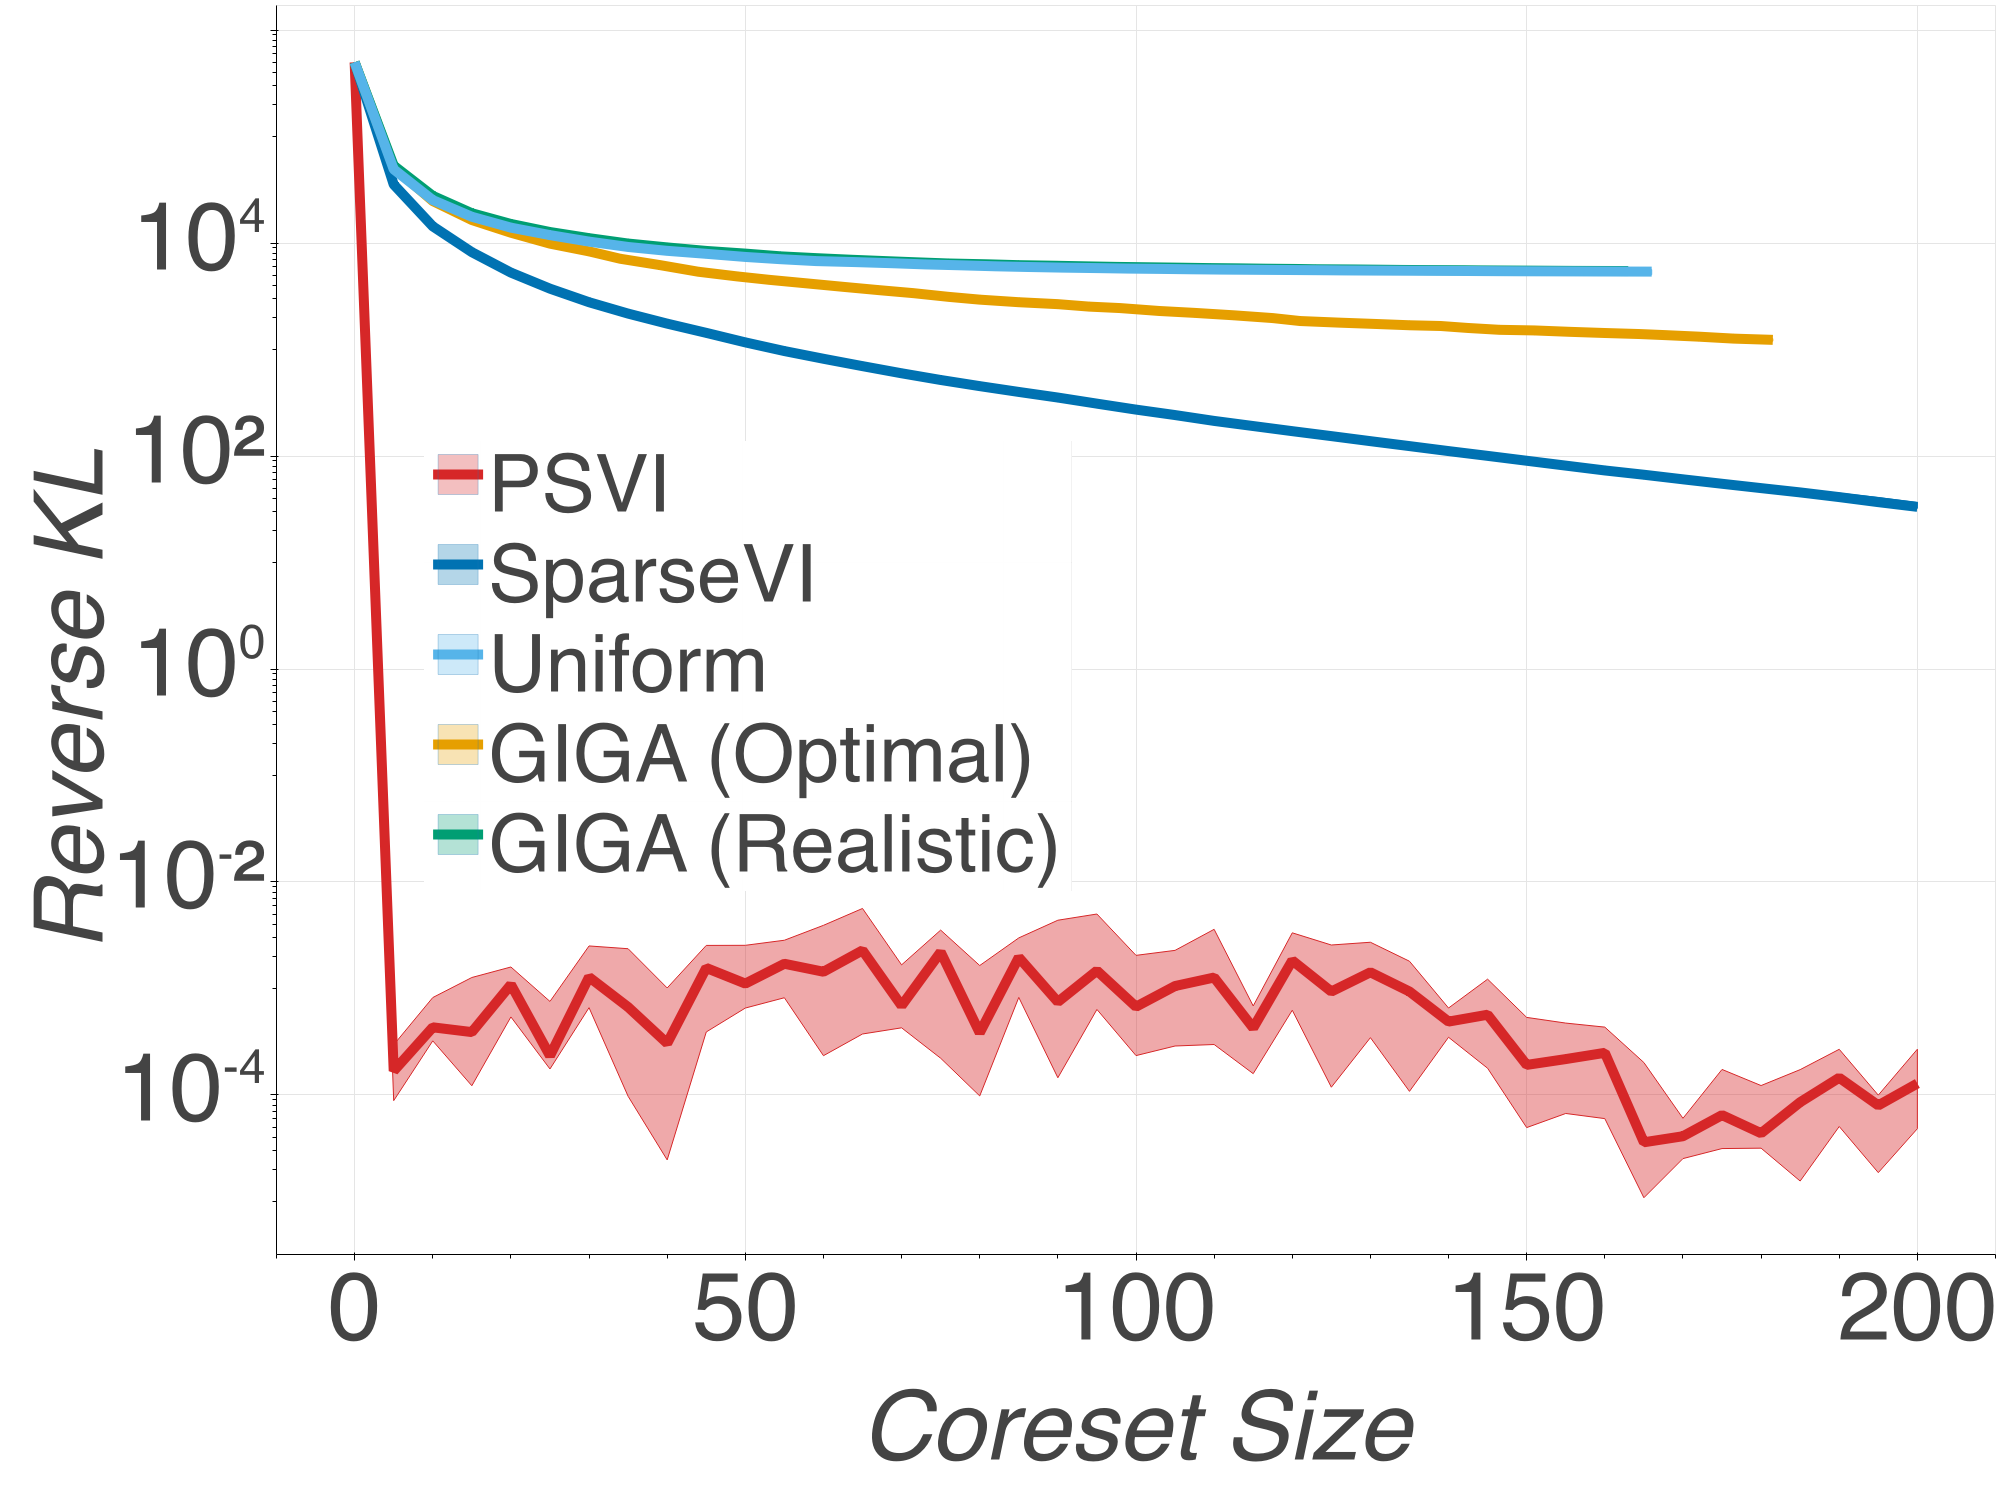
\includegraphics[width=.49\textwidth]{figs/d500_KLDvsCstSize.png}
\end{frame}

\begin{frame}
	\frametitle{Experiments II~(Bayesian Linear Regression)}
	\centering
	\begin{columns}
		\begin{column}{.5\textwidth}
		$\circ$ Synthetic dataset
		\\---101 dimensions,
		\\---2K datapoints
		\end{column}
		\begin{column}{.5\textwidth}
		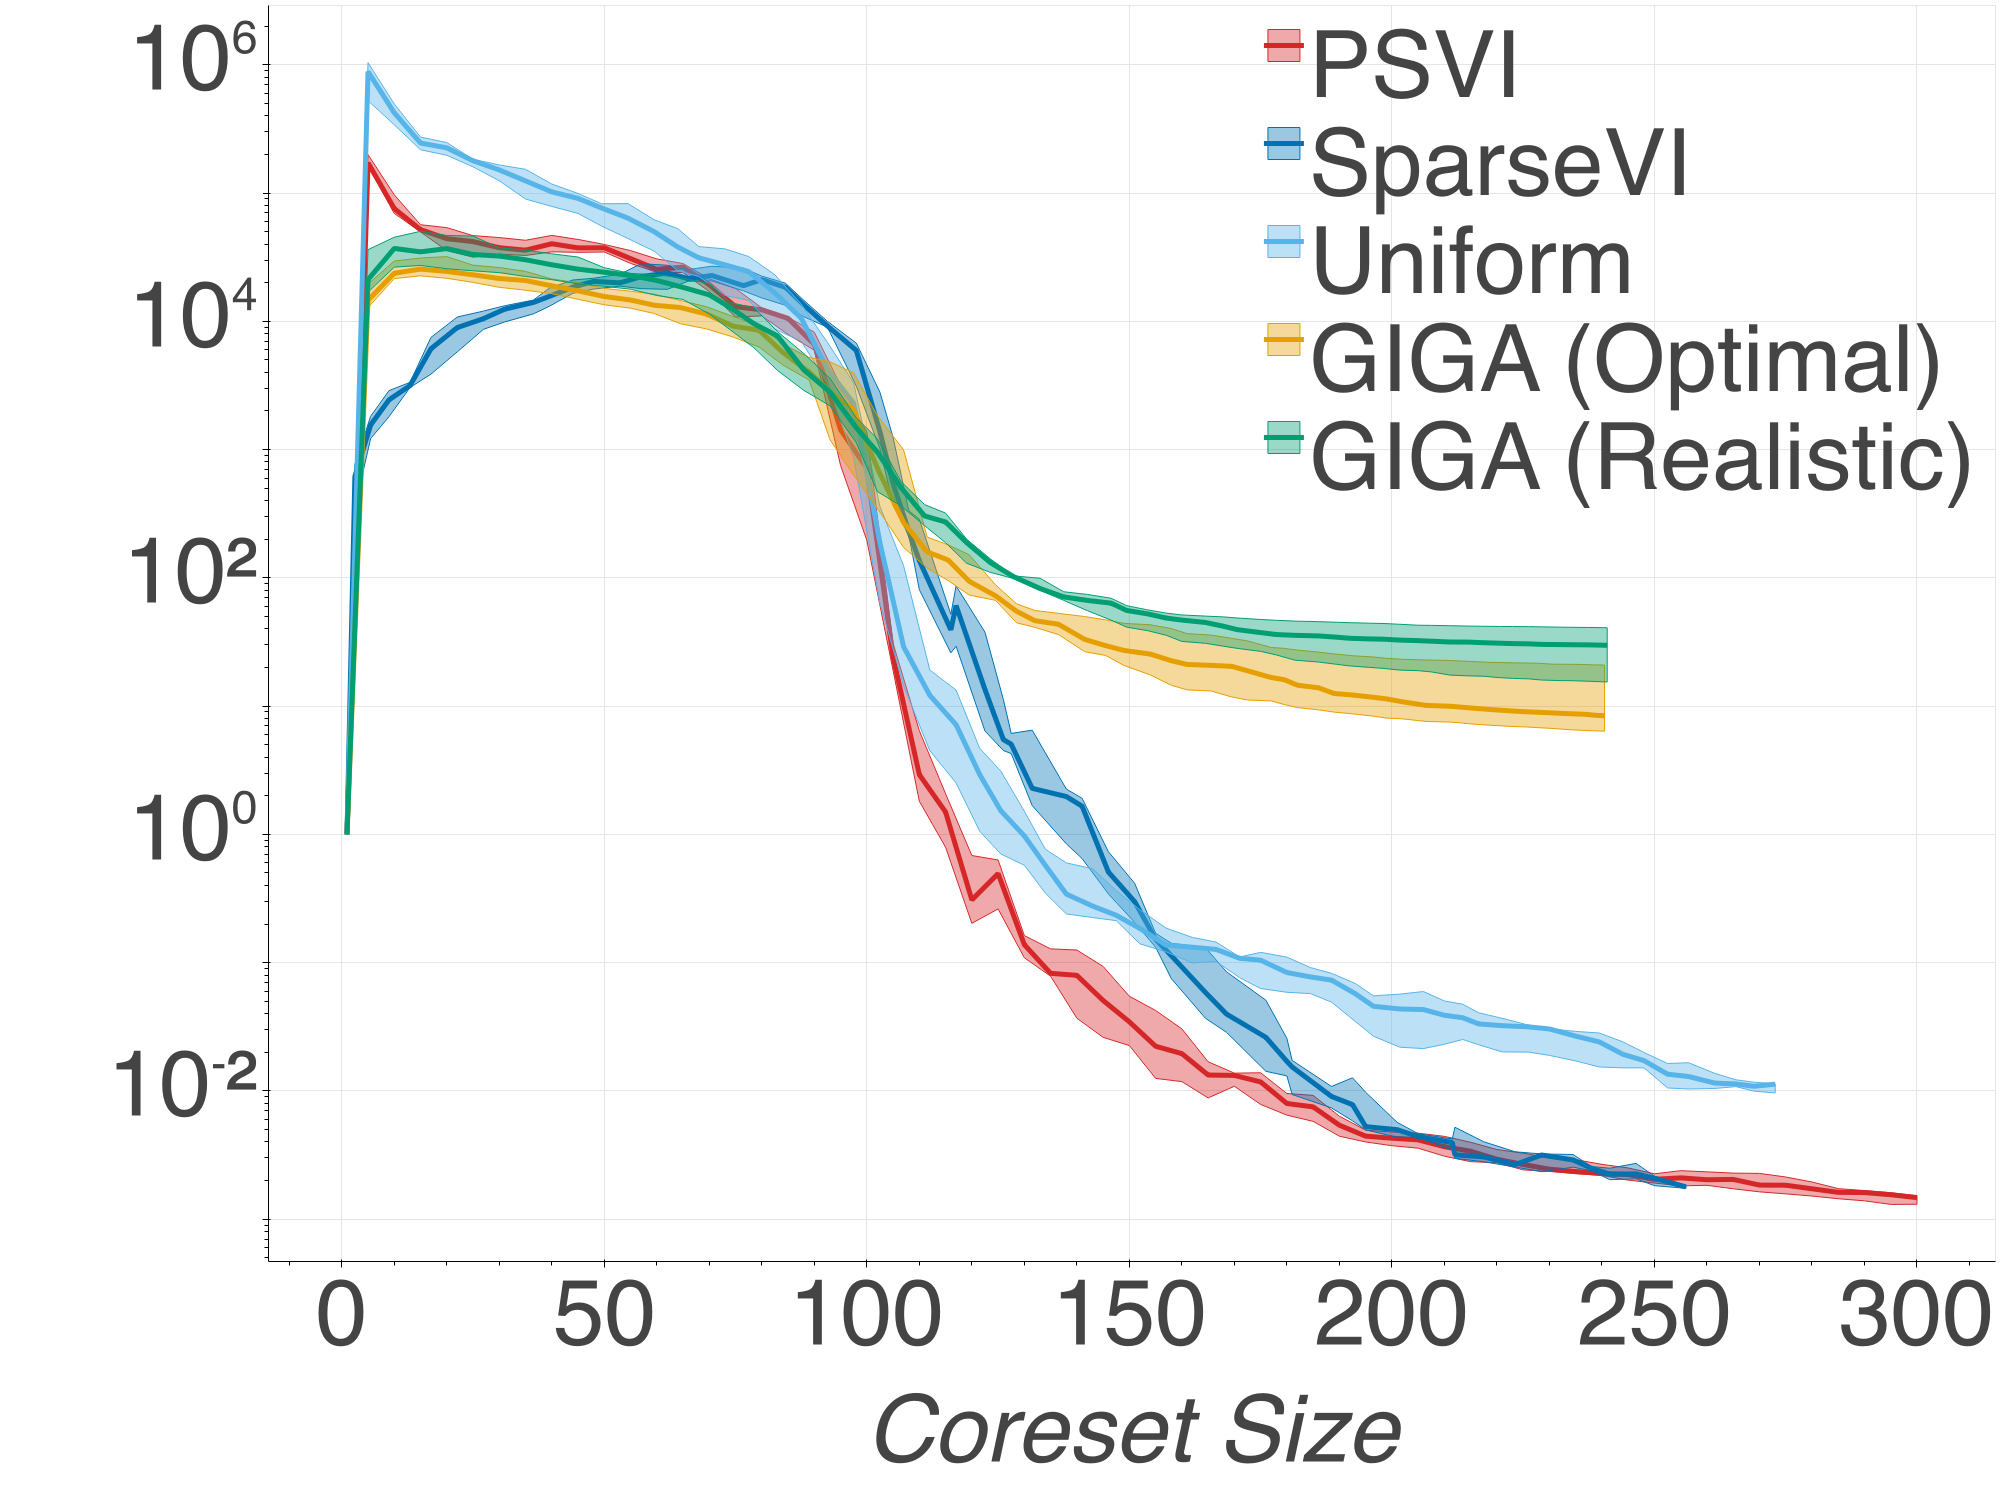
\includegraphics[width=1.\textwidth]{figs/linregKLDvsCstSize.png}
		\end{column}
	\end{columns}
\end{frame}

\begin{frame}
	\frametitle{Experiments III~(Bayesian Logistic Regression)}
	\centering 
	$\circ$ 2-237 dimensions, 500-100K datapoints\\
	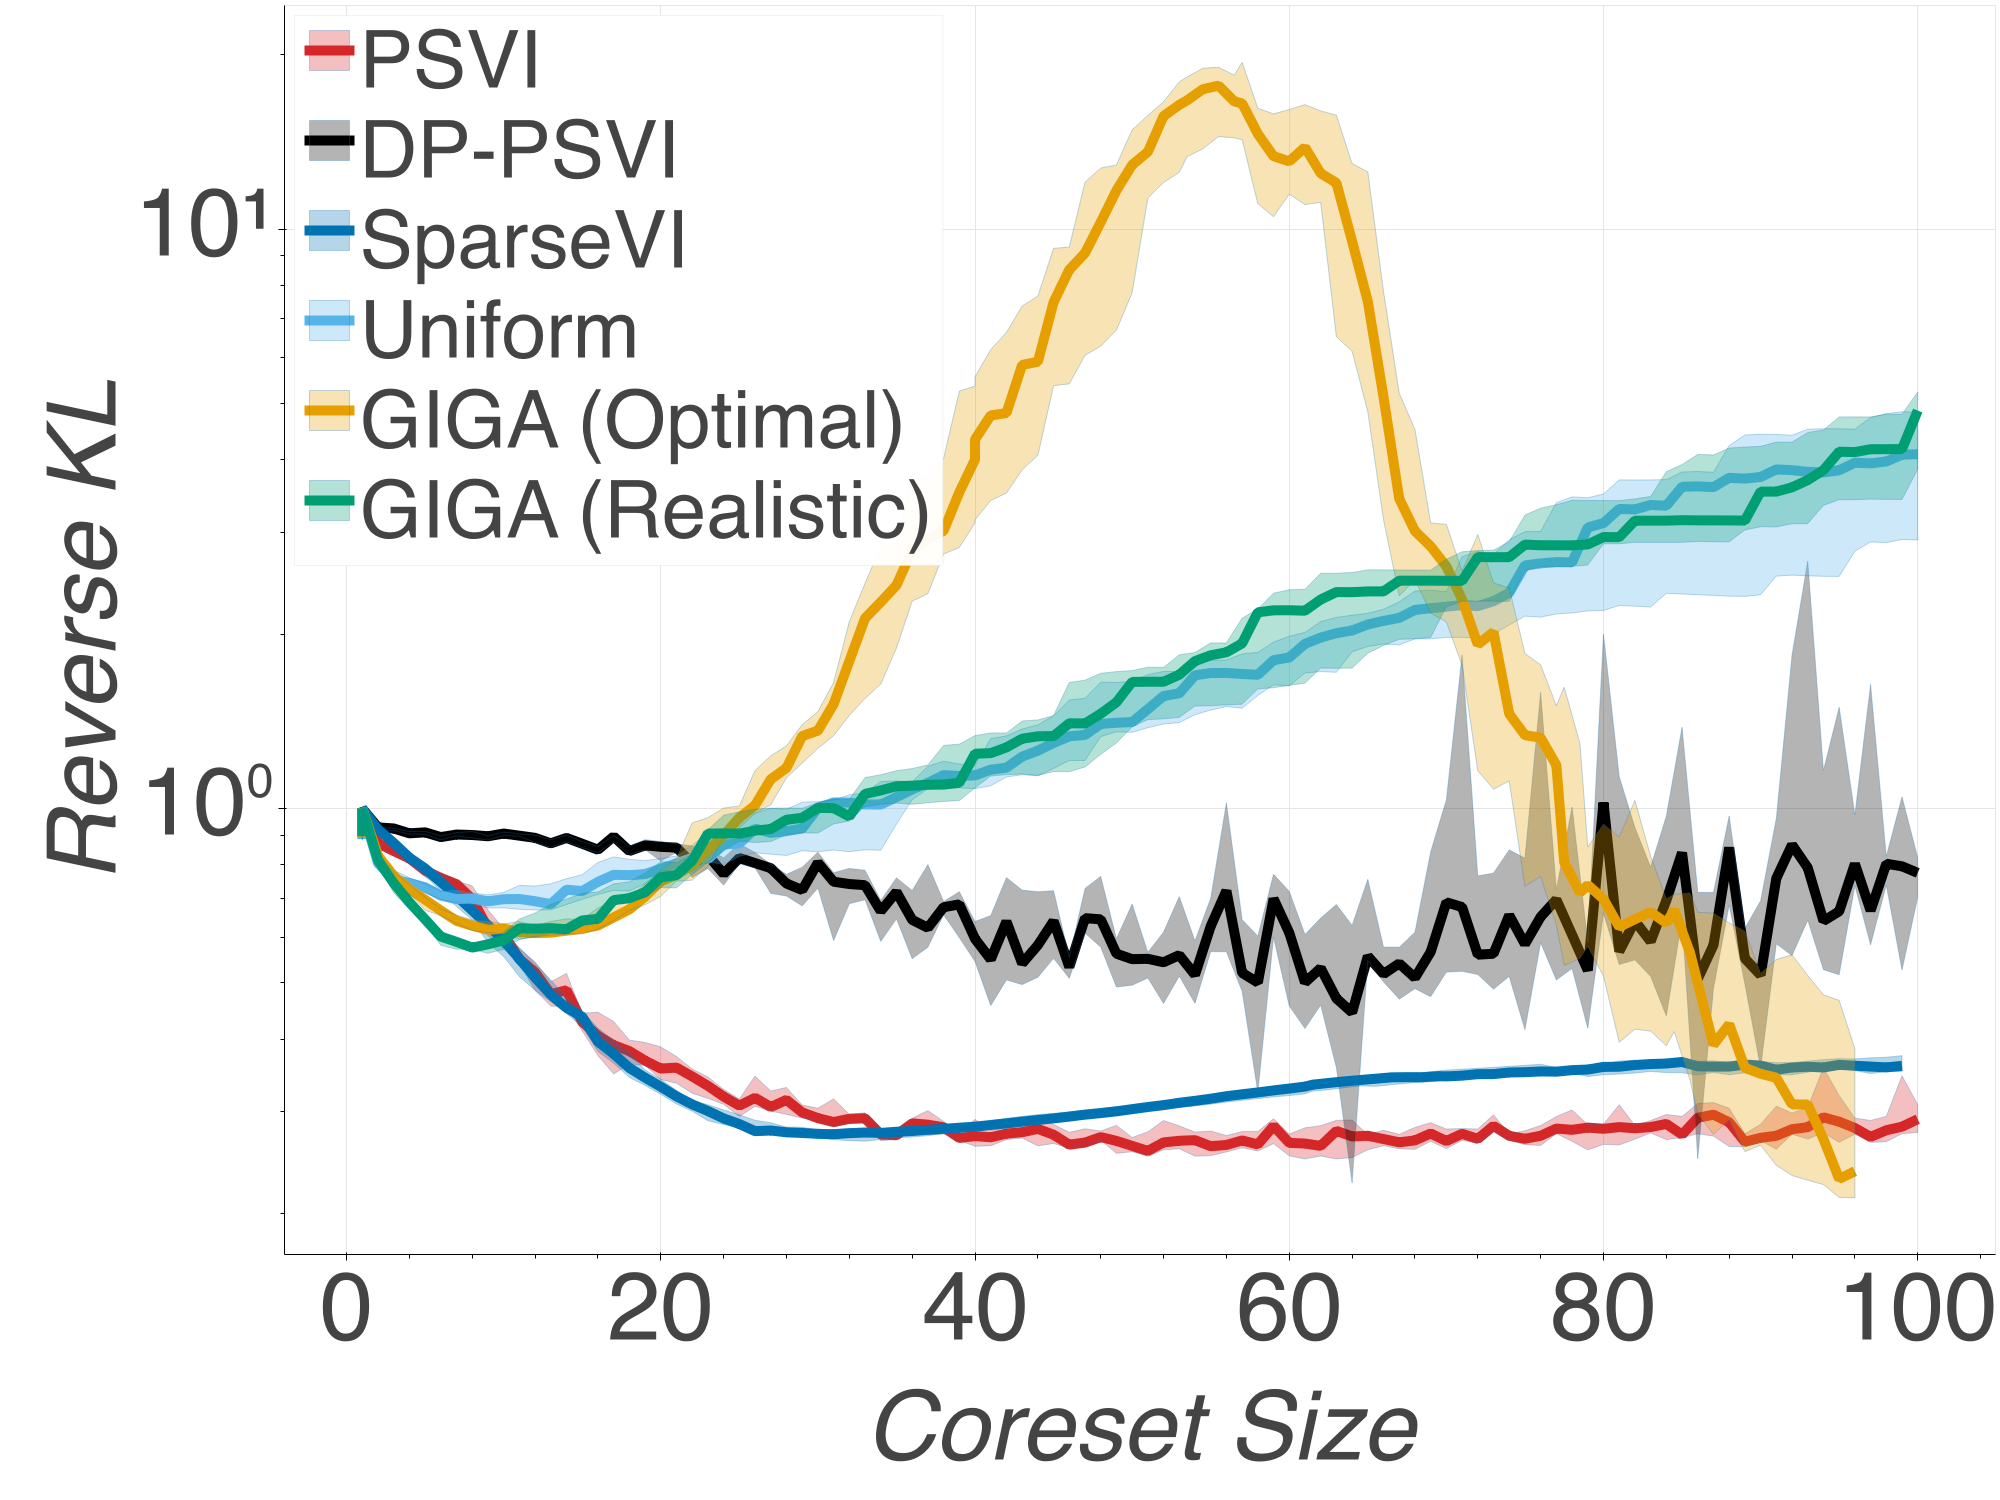
\includegraphics[width=.3\textwidth]{figs/wsanta100K_KLDvssz.png}
	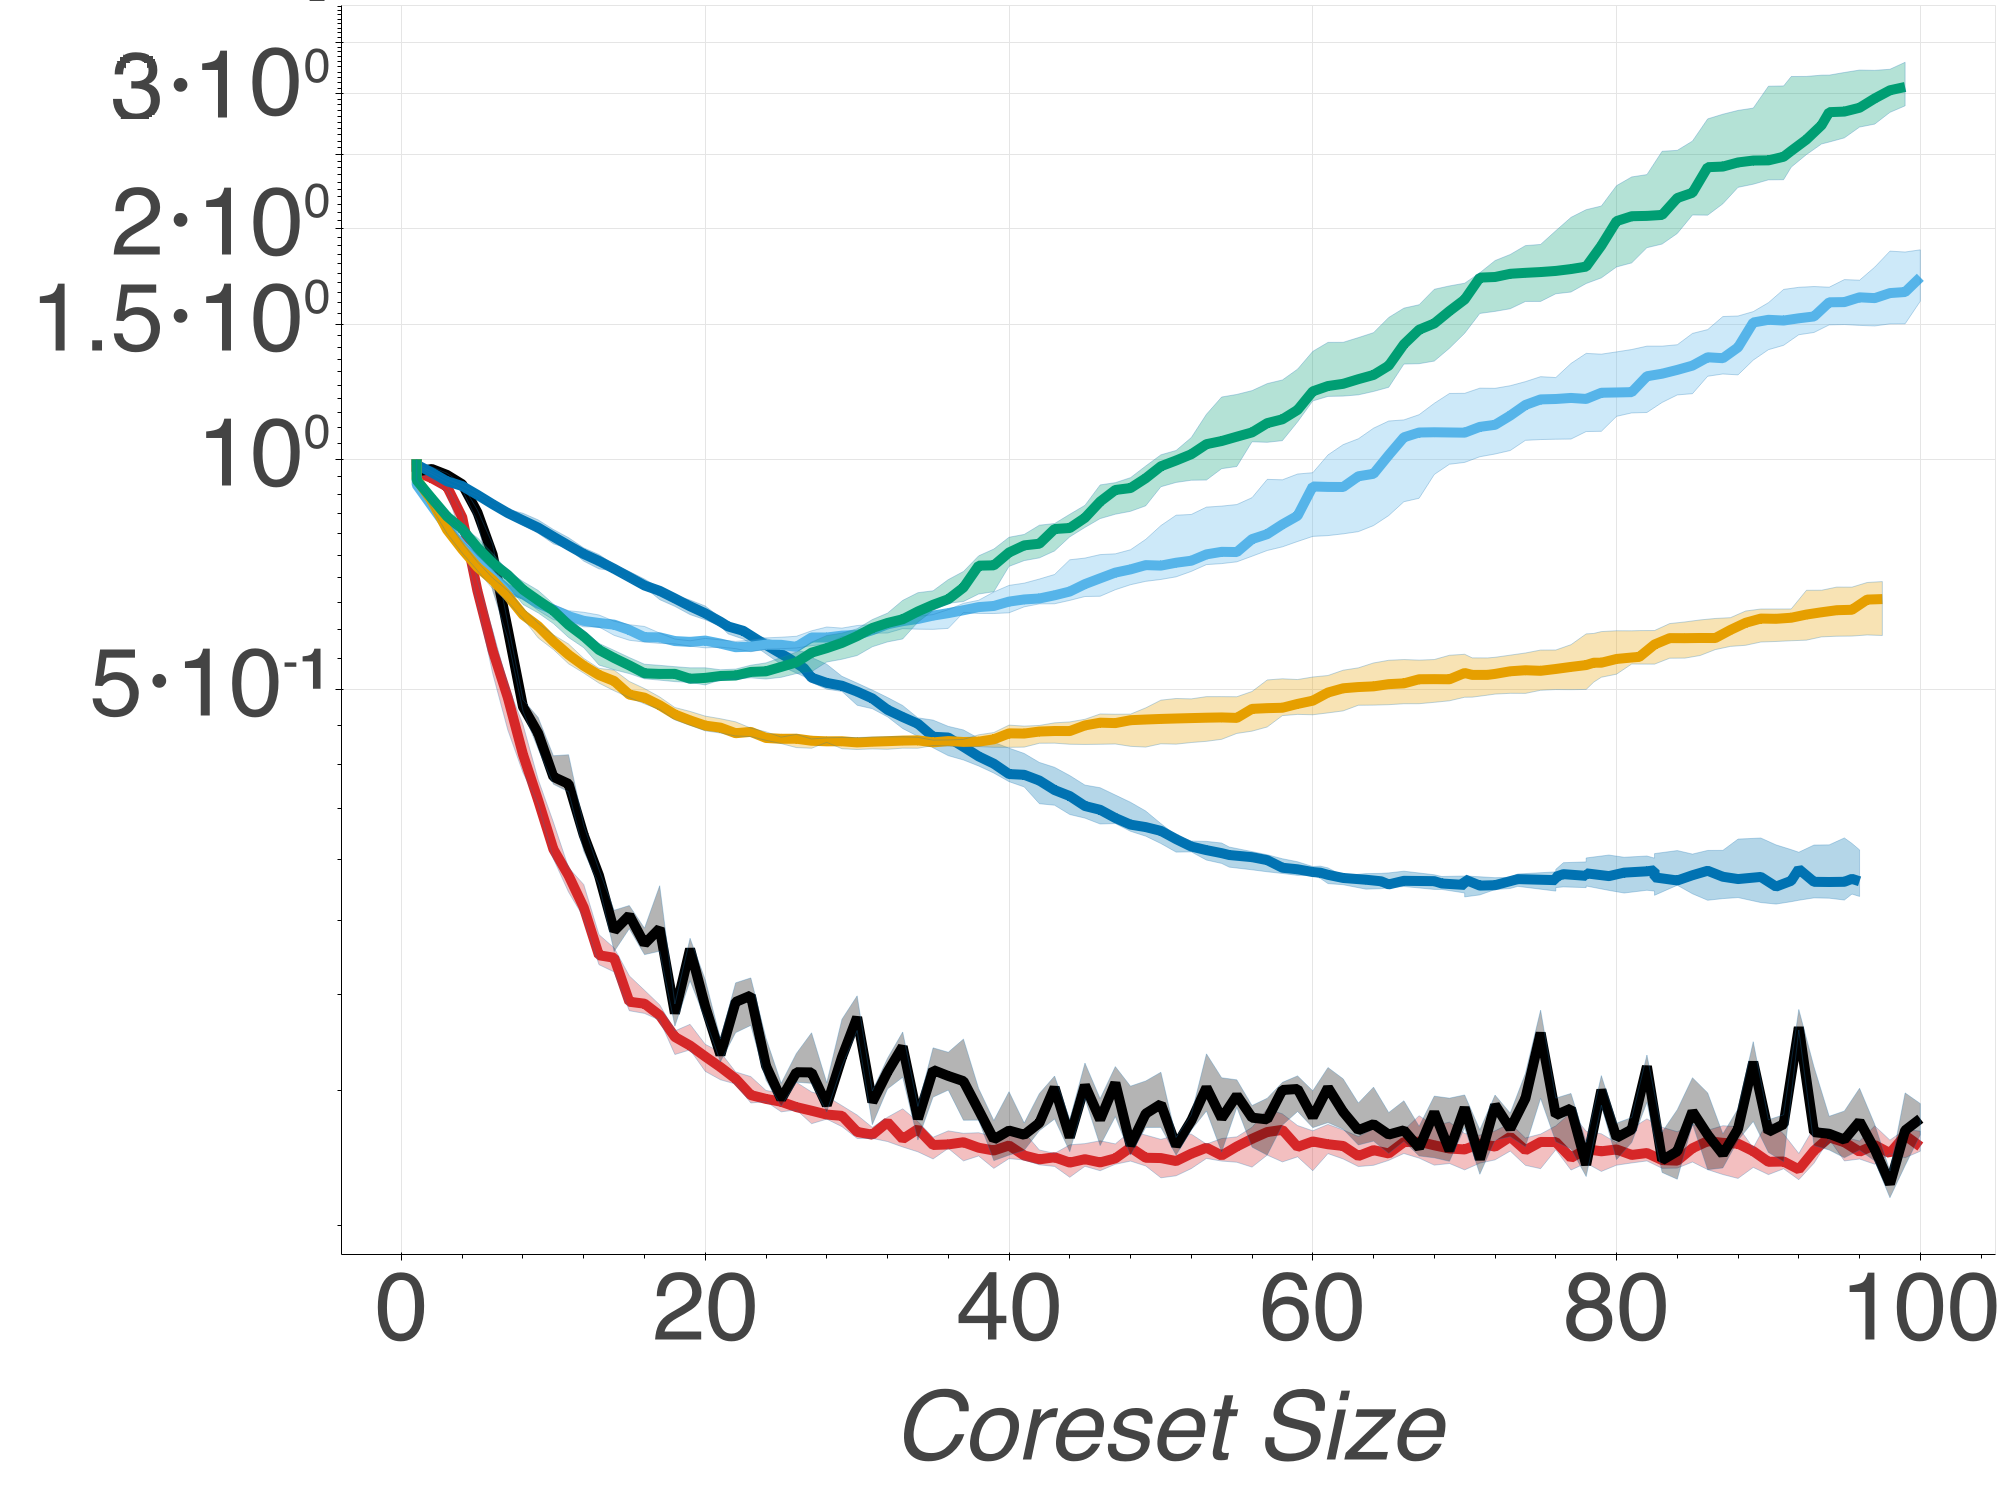
\includegraphics[width=.3\textwidth]{figs/wds1100_KLDvssz.png}
	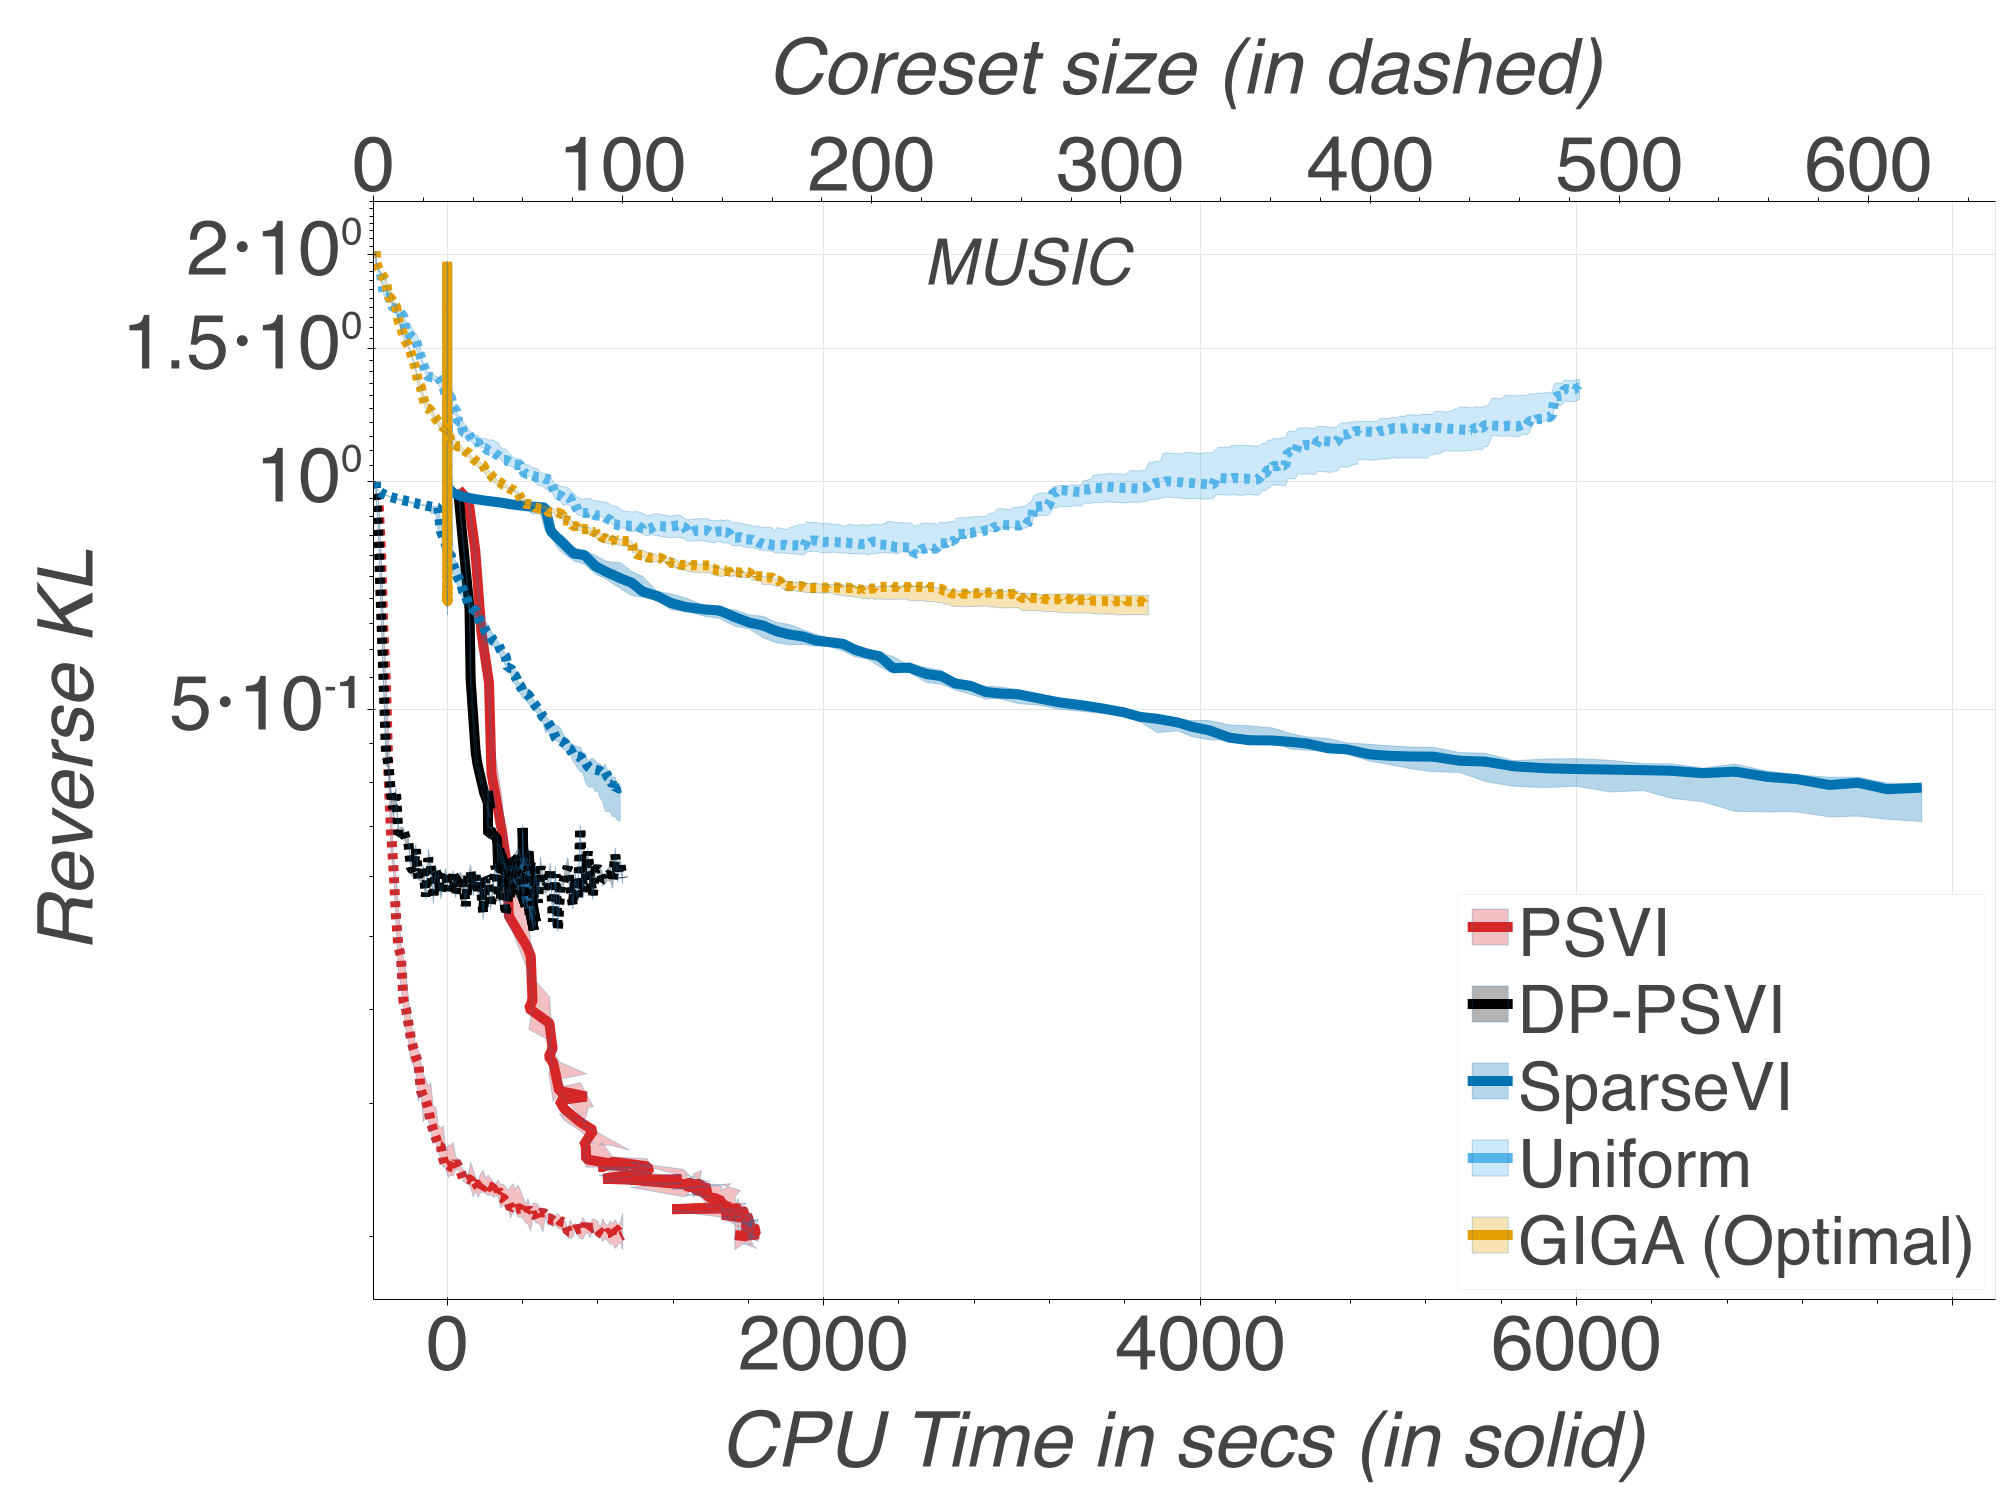
\includegraphics[width=.3\textwidth]{figs/fma_KLDvscput.png} \\
	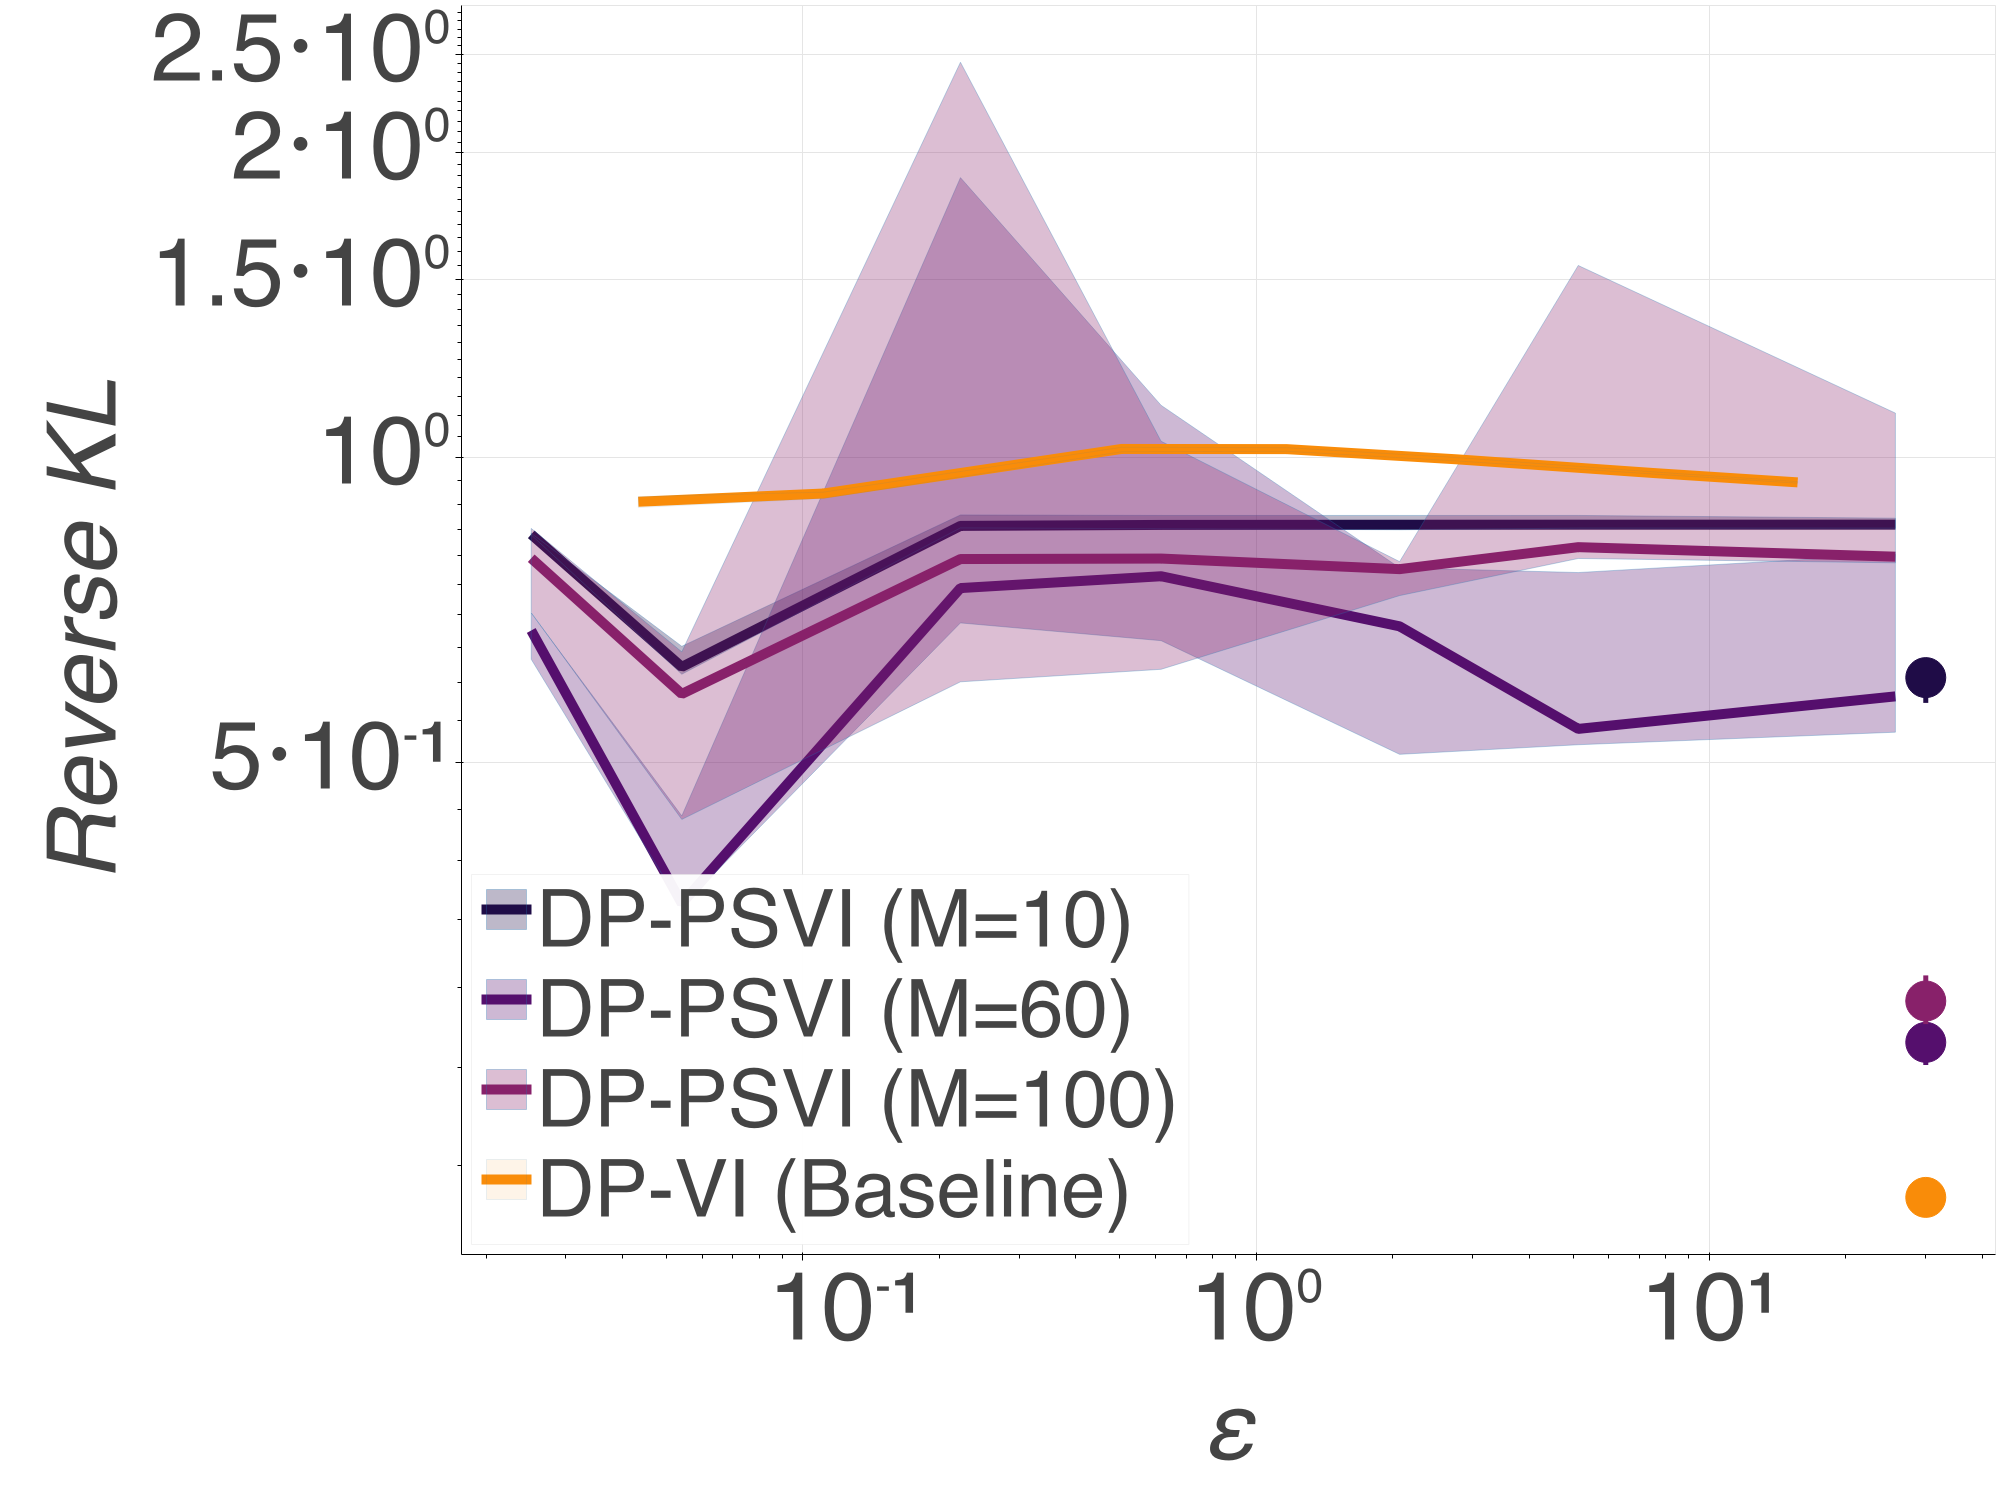
\includegraphics[width=.3\textwidth]{figs/wsanta100K_privacy.png}
	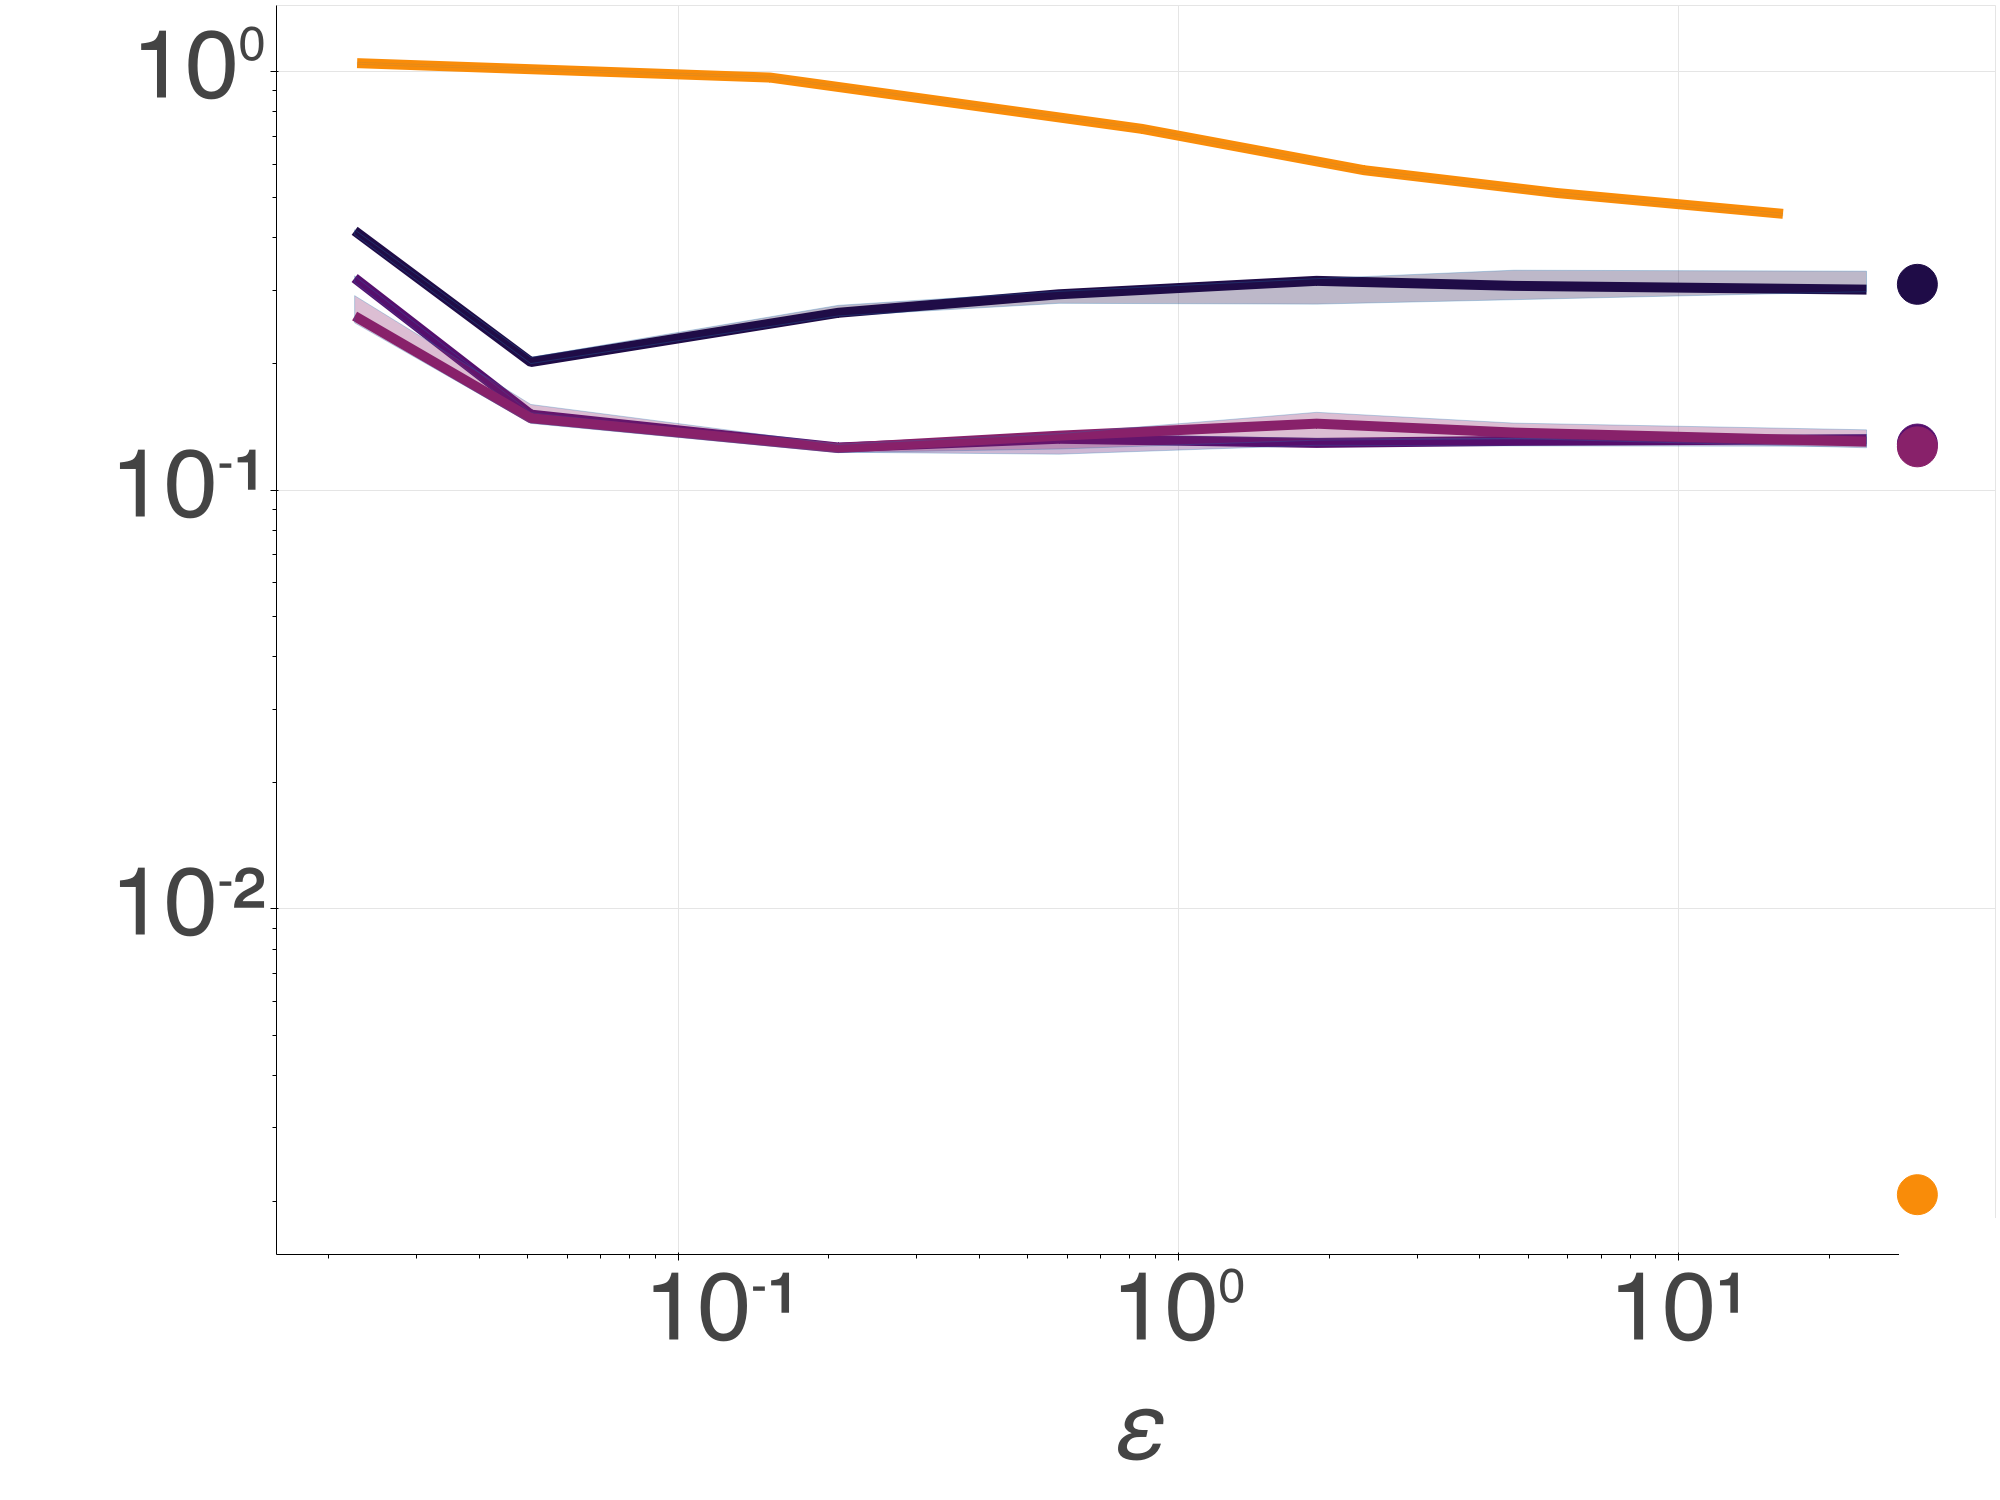
\includegraphics[width=.3\textwidth]{figs/wds1100_privacy.png}
	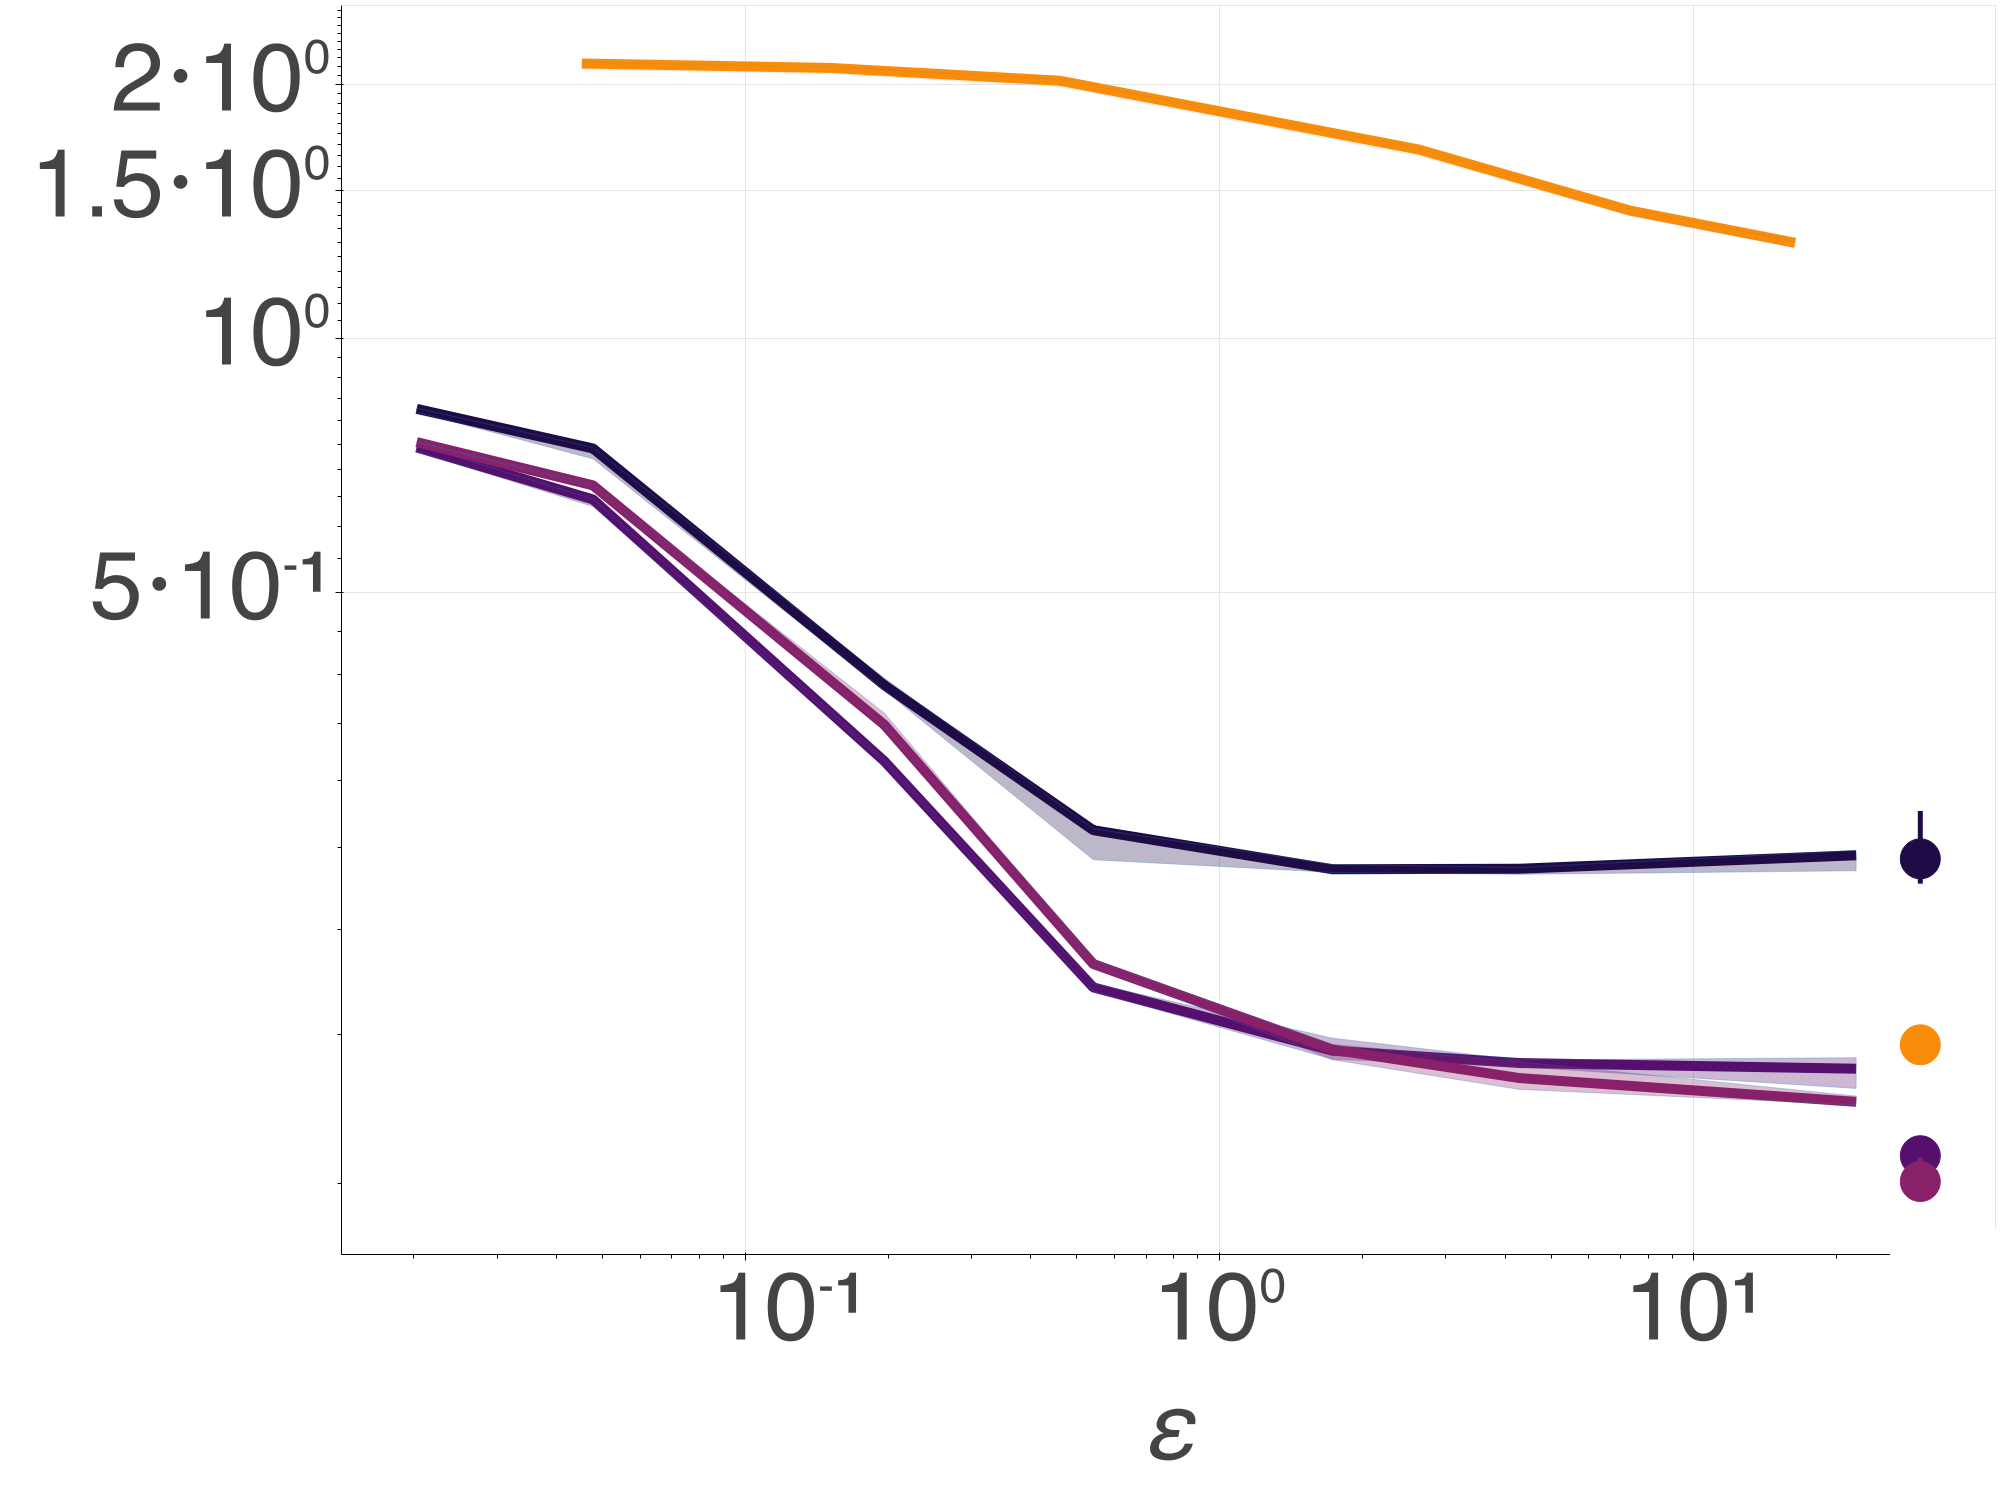
\includegraphics[width=.3\textwidth]{figs/wfma_privacy.png} 
	\small $\delta=\frac{1}{N}$
	\normalsize
\end{frame}




%%%%%%%%%%%%%%%%%%%%%%%%%%%%%%%%%%%%%%%%%%%%%%%%%%%%%%%
%%%%%%%%%%%%%%%%%%%%%%%%%%%%%%%%%%%%%%%%%%%%%%%%%%%%%%%
%% WSDM
%%%%%%%%%%%%%%%%%%%%%%%%%%%%%%%%%%%%%%%%%%%%%%%%%%%%%%%
%%%%%%%%%%%%%%%%%%%%%%%%%%%%%%%%%%%%%%%%%%%%%%%%%%%%%%%


\begin{frame}
	\LARGE{\textbf{II. $\beta$-Cores: Robust large-scale Bayesian data summarization in the presence of outliers}}
\end{frame}





\begin{frame}[fragile,t]
	\frametitle{Challenges}
	\begin{columns}[onlytextwidth]
		\begin{column}{0.35\textwidth}  %%<--- here
			\vspace{-1cm} 
			
			\begin{center}
				\begin{figure}
					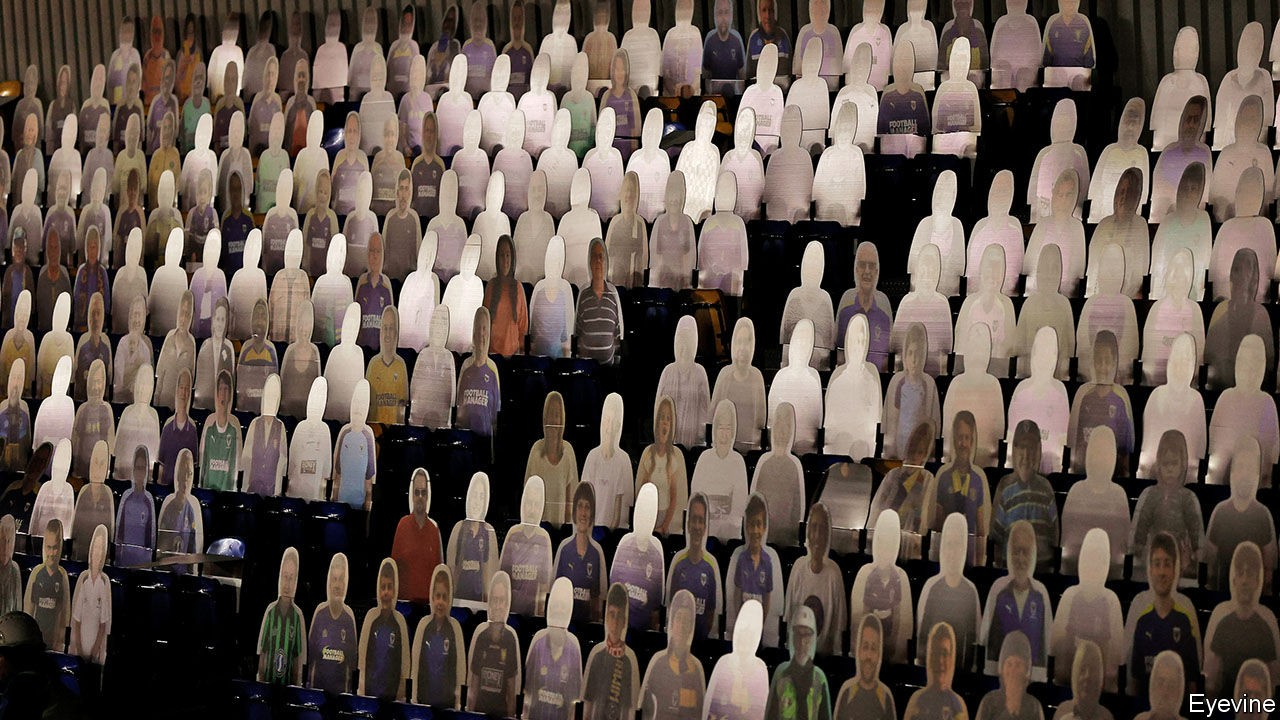
\includegraphics[width=0.9\textwidth,angle=5]{figs/crowds.jpg}
				\end{figure}
				
				\vspace{-.35cm} 
				
				\begin{figure}
					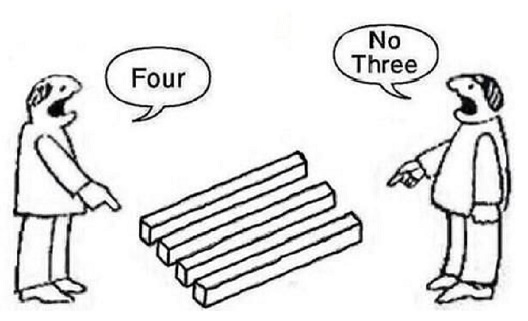
\includegraphics[width=0.9\textwidth,angle=-5]{figs/Four-No-Three.jpg}
					\caption*{The Hierarchy of Disagreement by Paul Graham}
				\end{figure}
				
				\vspace{-.35cm} 
				
				\begin{figure}
					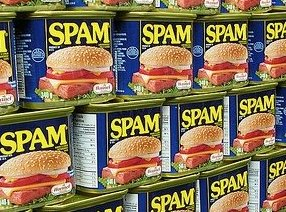
\includegraphics[width=0.9\textwidth,angle=-5]{figs/spam.jpg}
				\end{figure}
			\end{center}
		\end{column}
		\begin{column}{0.65\textwidth}
			\vspace{-2.6cm} 
			
			\begin{itemize}
				\item $\blacktriangleright$ Web-scale ML systems on \emph{\textbf{massive}} data from \emph{\textbf{multiple sources}}
				\item $\blacktriangleright$ \textbf{Requirement 1}: \emph{Scalability}  via reducing redundancy
				\item $\blacktriangleright$ \textbf{Requirement 2}: \emph{Robustness to statistical misspecification} caused by observations, and/or model assumptions   
				\item $\blacktriangleright$ \textbf{$\beta$-Cores}: summarizations robust to contamination as an \textbf{integrated approach to data cleaning \emph{and} scalable inference} with high automation
			\end{itemize}
		\end{column}
	\end{columns}
\end{frame}

\begin{frame}
	\frametitle{Background}
	$\blacktriangleright$ \textbf{Outliers} are typically 
	\begin{itemize}
		\item $\circ$ treated \textcolor{blue}{separately from inference}, and
		\item $\circ$ tackled via \textcolor{blue}{computing distances} within datapoints~\citep{diakonikolas19, dickens20}, or
		\item $\circ$ introducing \textcolor{blue}{data redudancies}~\citep{raykar10, karger11}.
	\end{itemize} 
	\pause
	$\blacktriangleright$ Such approaches \emph{\textbf{scale adversely}} with data \textbf{dimensionality} and \textbf{size}, often decreasing automation or imposing assumptions on outliers.
\end{frame}

\begin{frame}
	\frametitle{Background}
	$\blacktriangleright$ \textbf{Robustified Bayesian inference} via 
	\begin{itemize}
		\item --- \textcolor{blue}{heavy-tailed data likelihood functions}~\citep{huber09, insua12}
		\item --- \textcolor{blue}{localization}~\citep{definetti61, wang18}
		\item --- \textcolor{blue}{data reweighting}~\citep{wang17} 
		\item --- \textcolor{blue}{robust gradient estimates in MC methods}~\citep{bhatia19}
		\item --- \textcolor{blue}{pseudo-Bayesian posteriors with reduced sensitivity}: robust divergences, coarsening~\citep{futami18, knoblauch18, miller19}
	\end{itemize}
	\begin{figure}
		\begin{center}
			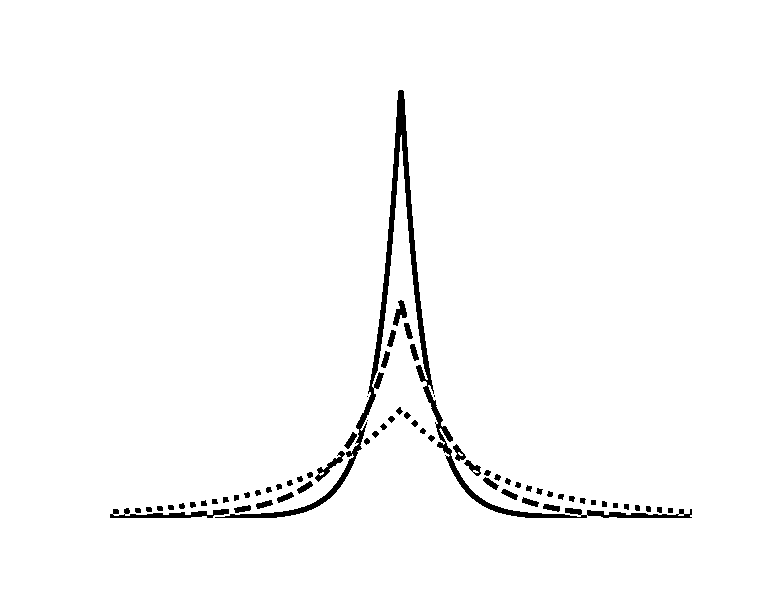
\includegraphics[width=0.24\textwidth,valign=c]{figs/heavy_tails.eps}
			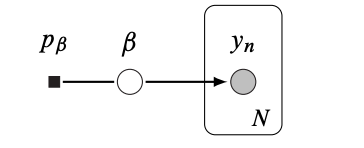
\includegraphics[width=0.24\textwidth,valign=c]{figs/original.png}
			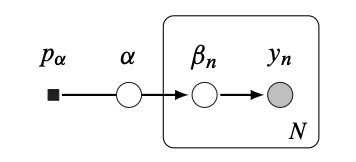
\includegraphics[width=0.24\textwidth,valign=c]{figs/localized.png}
			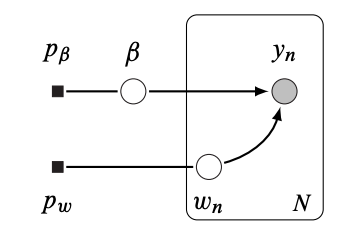
\includegraphics[width=0.24\textwidth,valign=c]{figs/reweighted.png}
		\end{center}
	\end{figure}
	\qquad heavy-tails \qquad\qquad \qquad\qquad\quad localization \qquad reweighting
	
\end{frame}




\begin{frame}
	\frametitle{Bayes' theorem: An optimization perspective}
	\centering 
	\begin{columns}
		\begin{column}{.79\textwidth}
			Bayes' rule as an optimization problem~\citep{zellner88}
		\end{column}
		\begin{column}{.29\textwidth}
			\hfill 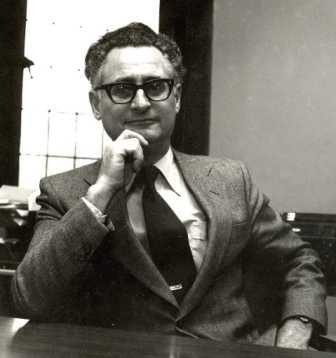
\includegraphics[width=1.\textwidth]{figs/Zellner.jpg}\\ 
		\end{column}
	\end{columns}
	\begin{equation*}
	\arg \underset{q(\theta) \in \mcP}{\min}  \left(\kl{q(\theta)}{\pi_0(\theta)} + \bm{N}\EE_{q(\theta)}\left[\kl{\hpi(x)}{\pi(x|\theta)}\right]\right),
	\end{equation*}
	giving
	\begin{align*}
	\pi(\theta|x) = \frac{1}{Z'} \exp\left(-\xent{\hpi(x)}{\pi(x|\theta)}\right)\pi_0(\theta),
	\end{align*}
	where $\hpi(x):=\frac{1}{N}\sum_{n=1}^{N}\delta(x-x_n)$ and $\xent{\hpi(x)}{\pi(x|\theta)}:=-\sum_{n=1}^{N}\log\pi(x_n|\theta)$~(cross-entropy).\\
	\emph{"Cost"} of the observations \emph{under the KL divergence}. 
\end{frame}


\begin{frame}
	\frametitle{Generalized Bayesian inference via $\beta$-divergence}
	$\blacktriangleright$ \textbf{Replace the KL} with the \emph{$\beta$- or density power divergence}~\citep{basu98}.
	\begin{align*}
	\arg \underset{q(\theta) \in \mcP}{\min}  \left(\kl{q(\theta)}{\pi_0(\theta)} + \bm{N}\EE_{q(\theta)}\left[\db{\hpi(x)}{\pi(x|\theta)}\right]\right),
	\end{align*}
	$\blacktriangleright$ \textbf{$\beta$-posterior}~\citep{futami18}:
	\begin{align*}
	\pi_\beta(\theta|x) \propto \exp\left(-\db{\hpi(x)}{\pi(x|\theta)}\right)\pi_0(\theta),
	\end{align*}
	where \\
	$\db{\hpi(x)}{\pi(x|\theta)} := -\sum_{n=1}^{N}  \underbrace{\left(\frac{\beta+1}{\beta}\pi(x_n|\theta)^{\beta} + \int_{\mcX} \pi(\chi|\theta)^{1+\beta}d\chi\right)}_{:=f_n(\theta)}$, with $\beta>0$.
\end{frame}


\begin{frame}
	\frametitle{Generalized Bayesian inference via $\beta$-divergence}
		$\db{\hpi(x)}{\pi(x|\theta)} := -\sum_{n=1}^{N}  \underbrace{\left(\frac{\beta+1}{\beta}\pi(x_n|\theta)^{\beta} + \int_{\mcX} \pi(\chi|\theta)^{1+\beta}d\chi\right)}_{:=f_n(\theta)}$, with $\beta>0$.
	\begin{itemize}
		\item $\circ$ \emph{\textbf{solves robustness}}: different strengths of influence to each datapoint, downweighting outliers \cmark
		\item $\circ$ when $\beta \rightarrow 0$ \emph{\textbf{classical}} Bayesian posterior gets recovered
		\item $\circ$ \emph{\textbf{still difficult to compute}}:~same scalability issues with classical Bayesian posterior \color{red}{\xmark}
	\end{itemize}
\end{frame}

\begin{frame}
	\frametitle{Coresets for $\beta$-posterior}
	$\blacktriangleright$  \textbf{Sparse $\beta$-posterior}
	\begin{align*}
	\pi_{\beta,w}(\theta|x) 
	:= \frac{1}{Z(\beta, w)}  \exp\left(\sum_{n=1}^{N}w_nf_n(\theta)\right)\pi_0(\theta)
	\end{align*}
	$\blacktriangleright$  Variational formulation
	\begin{align*}
	w^{*} = \arg \min_{w\in\reals^{N}} \kl{\pi_{\beta,w}}{\pi_{\beta}} 
	\quad
	\text{s.t.}
	\quad
	w \geq 0,\; ||w||_0 \leq M.
	\end{align*}
	$\blacktriangleright$  Analytical gradients~\citep{campbell19neurips}
	\begin{align*}
	\nabla_{w}\kl{\pi_{\beta,w}}{\pi_\beta} 
	& = -\cov_{\beta,w}\left[f,(1 -w)^Tf\right],
	\end{align*}
	where $f:=\left[f_1(\theta) \ldots f_N(\theta)\right]^T$.
\end{frame}

\begin{frame}
	\frametitle{Optimization scheme}
	\begin{align*}
	\text{For } & m=1,\ldots,M\\
	&\text{(1)~Next datapoint selection~(\emph{Discrete optimization})} \\
	&m^\star = \underset{m\in[N]}{\argmin} \kl{\pi_{\beta, w \leftarrow w \cup \{x_m\}}}{\pi_\beta}\\
	&\text{(2)~Coreset reweighting~(\emph{Continuous optimization})}\\
	&w^\star = \underset{w \in \reals^{N}_{\geq 0}}{\argmin}\kl{\pi_{\beta, w}}{\pi_\beta}\\ 
	\end{align*}
\end{frame}


\begin{frame}
		\frametitle{Next datapoint selection}
		\begin{itemize}
			\item ---Ideally: select greedily, via maximizing locally the decrease in KL (\emph{ignoring the effects of reweighting step})
			\item ---Sample from all possible expansions: likely \emph{negligible effects}
			\item ---Generally objective is \emph{non-submodular}
			\item $\circ$ \textbf{Solution}: \emph{Maximize correlation} with residual error 
		\end{itemize}
		\begin{center}
		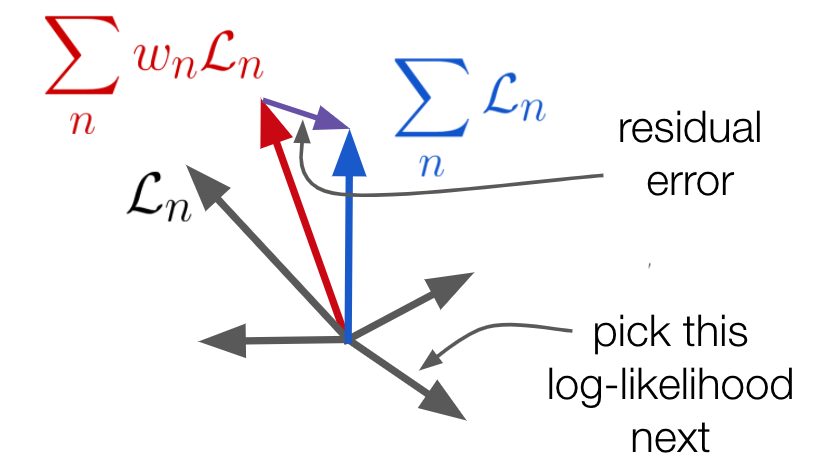
\includegraphics[width=5cm,height=3cm]{figs/next-point-selection.png}\\
		\end{center}
	$\blacktriangleright$ Works seamlessly when summarizing batches
\end{frame}


\begin{frame}
	\frametitle{2-step black-box incremental sparse approximation of the $\beta$-posterior}
	\begin{itemize}
		\item $\blacktriangleright$ Pseudocode sketch
		\scriptsize 
		\begin{tcolorbox}
			\begin{algorithmic}[1]
				\Procedure{\bcore}{$\beta$, likelihood function, coreset size $M$, minibatch size $B$, $\#$ of optimization steps $T$, $\#$ of samples from coreset iterates $S$}
				\LineCommentIndent{ \textbf{Initialize} from the prior}			 
				\For{$\text{coreset size~}m =1, \ldots, M $}
				\LineCommentIndent{Get $S$ samples from coreset posterior}\\
				\LineCommentIndent{\textbf{Select next coreset point} via max-correlation with residual error computed on a random minibatch from the full dataset}			 
				\For{$ t = 1, \ldots, T$}
				\LineCommentIndent{Get $S$ samples from coreset posterior}
				\LineCommentIndent{\textbf{Reweight} via Monte-Carlo gradient descent}
				\EndFor
				\EndFor
				\State\Return $w$%, $\beta$
				\EndProcedure		 
			\end{algorithmic}
		\end{tcolorbox}
		\normalsize
		\pause 
		\item $\blacktriangleright$ Computational complexity $O(M(M+B)ST)$
	\end{itemize}
\end{frame}

\begin{frame}
	\frametitle{Experiment I: Gaussian Mean Inference under Stuctured Data Contamination}
	\centering
	\includegraphics[width=.63\textwidth, height=4.35cm]{figs/gauss_scatterplot.png}\\
	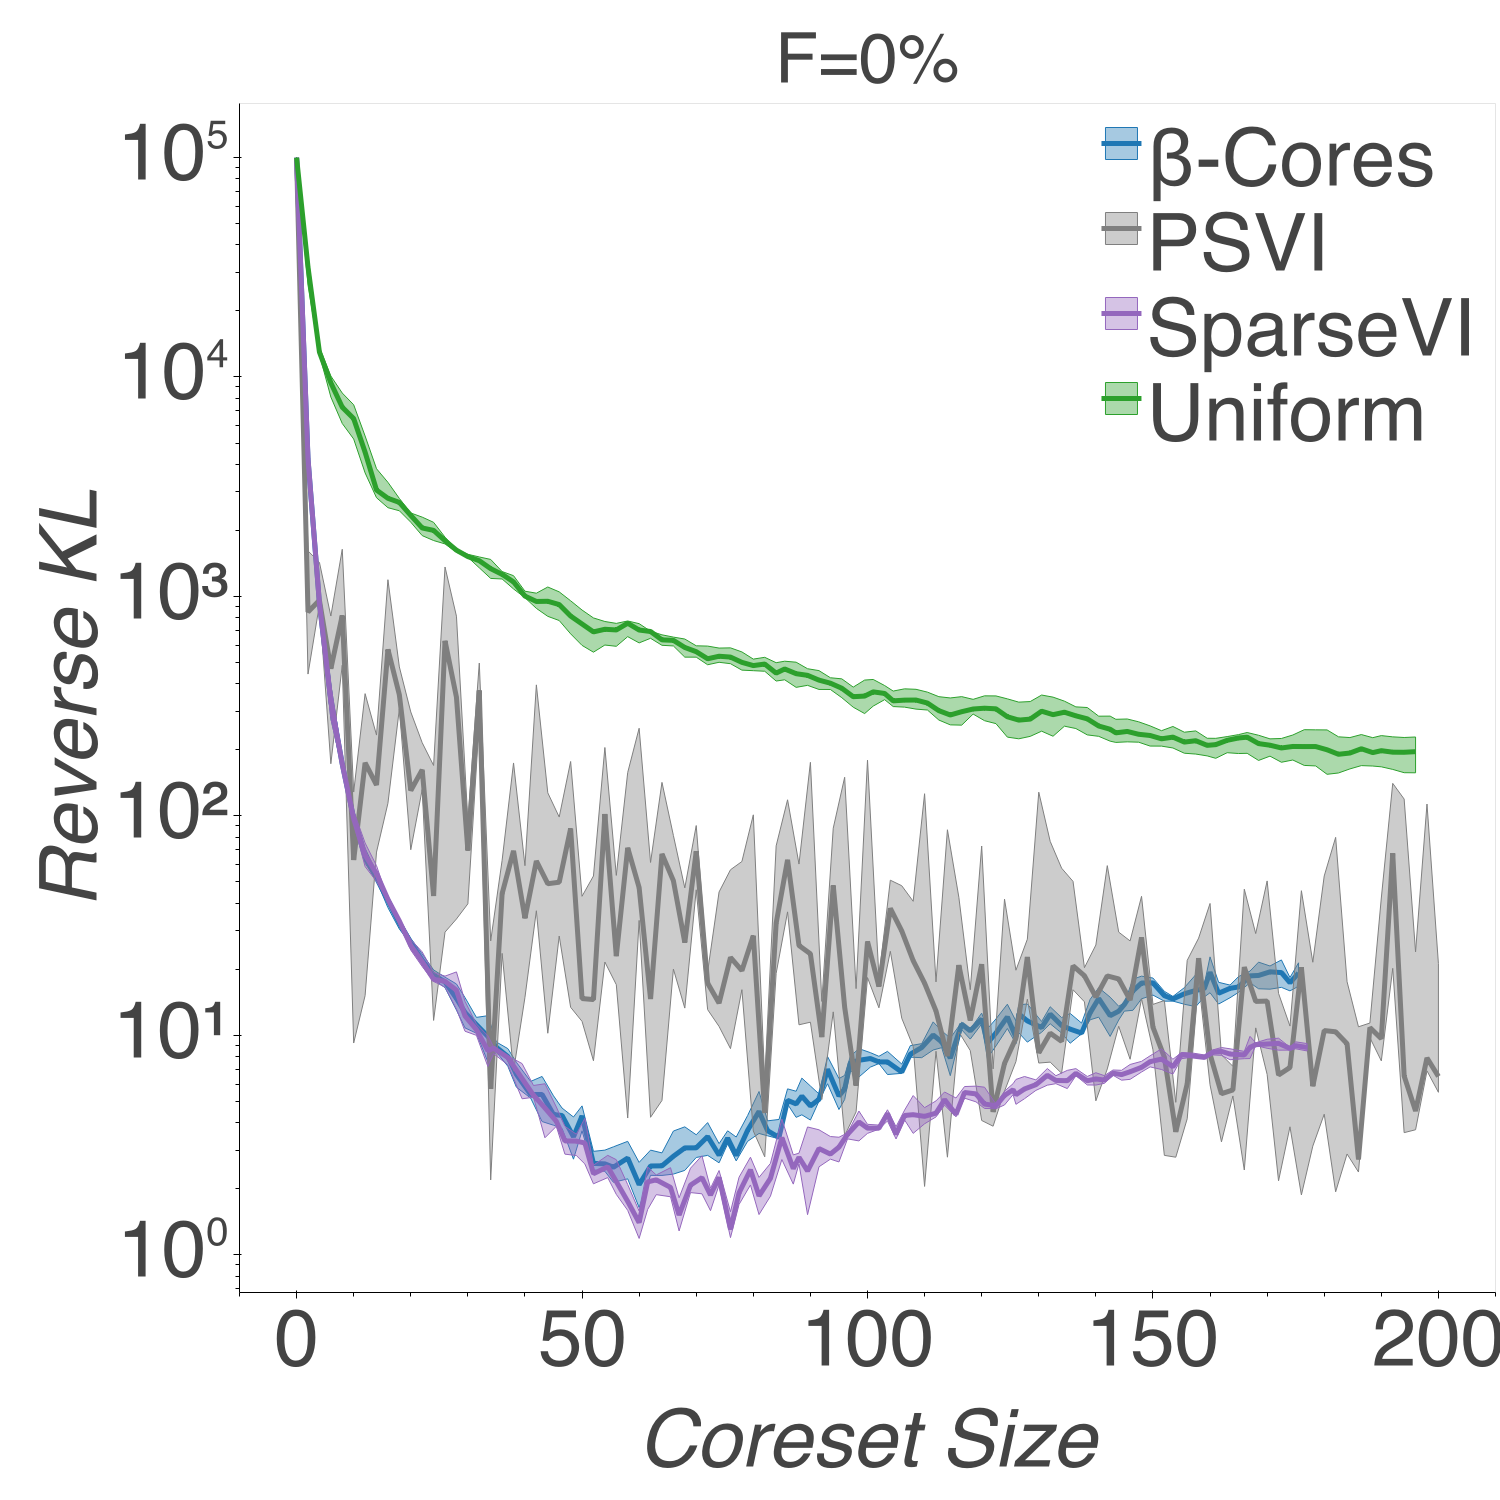
\includegraphics[width=.3\textwidth]{figs/f0KLDvsCstSize.png}
	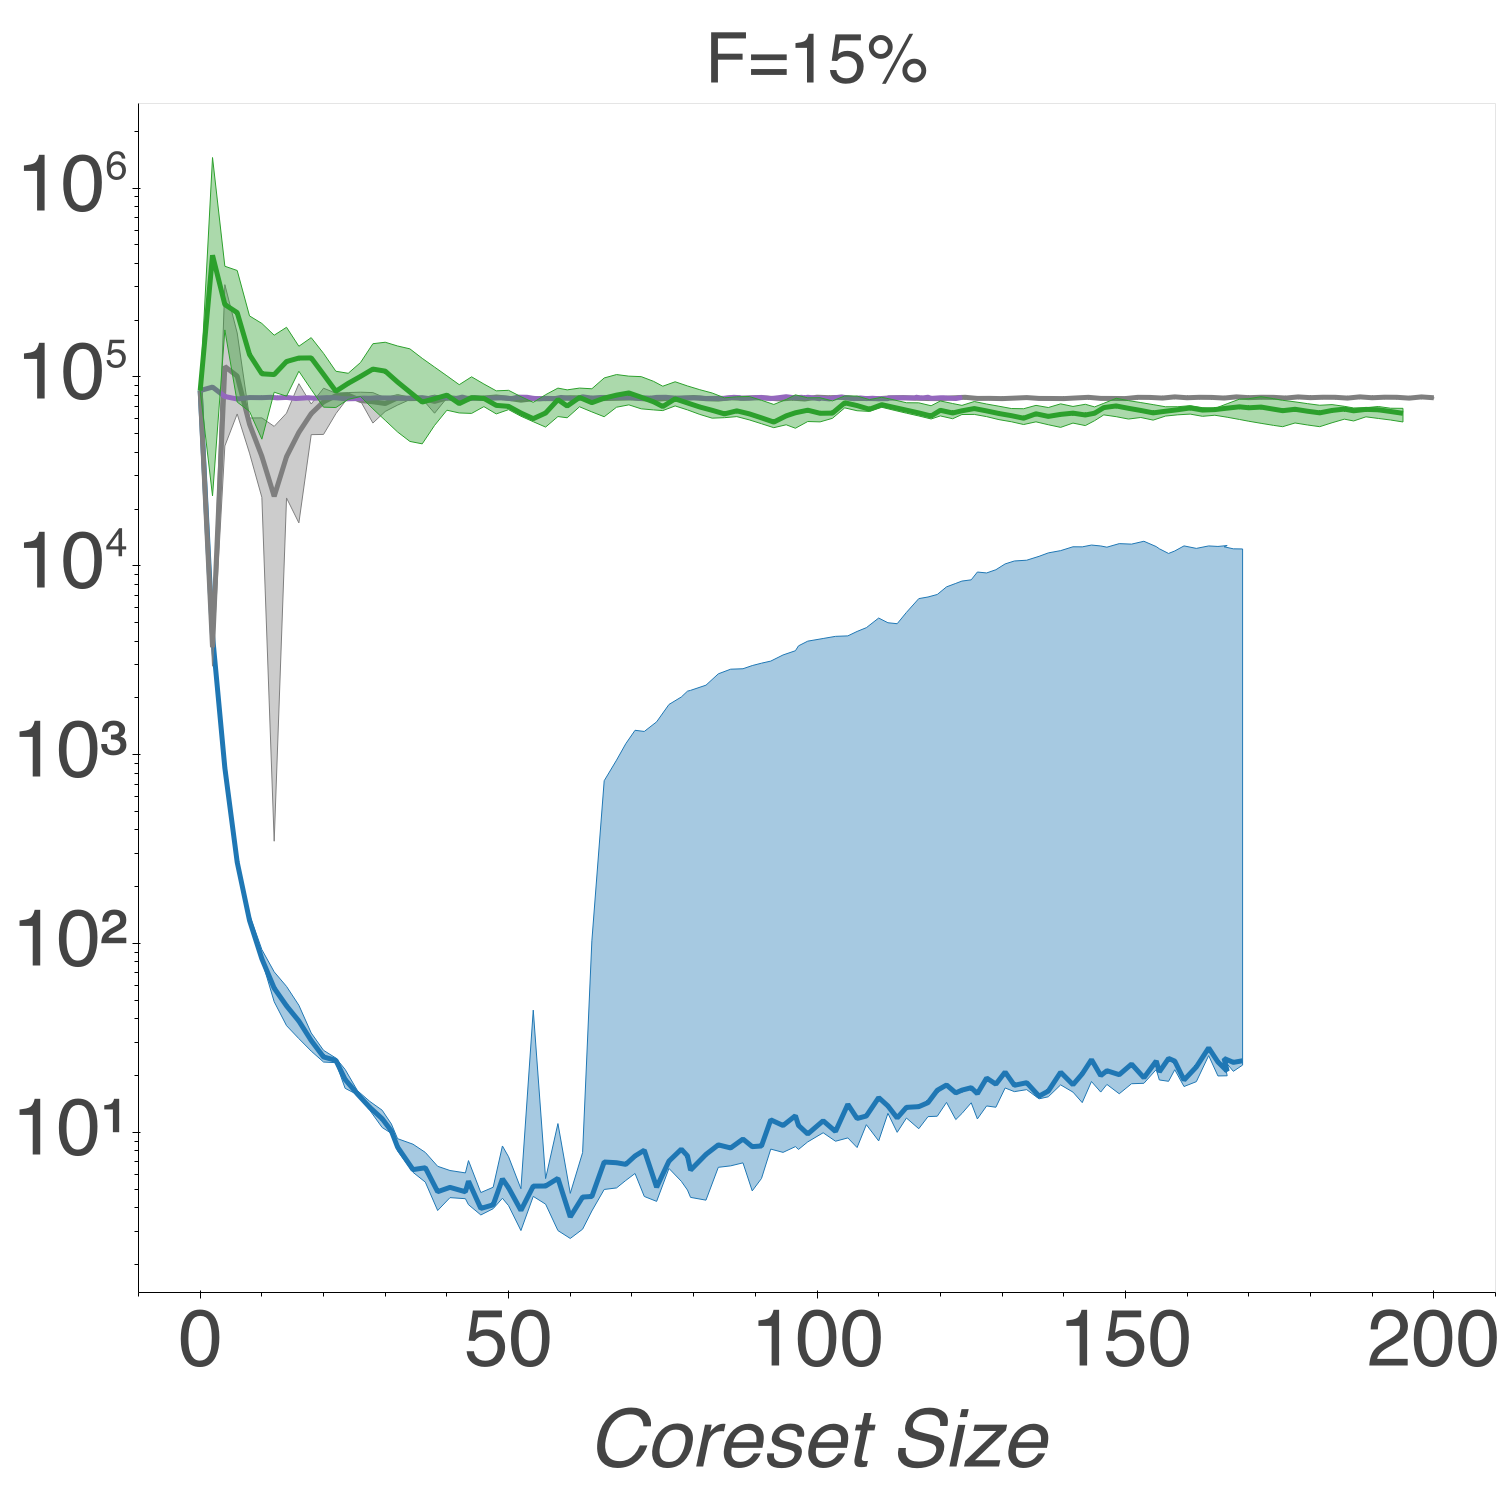
\includegraphics[width=.3\textwidth]{figs/f15KLDvsCstSize.png}
	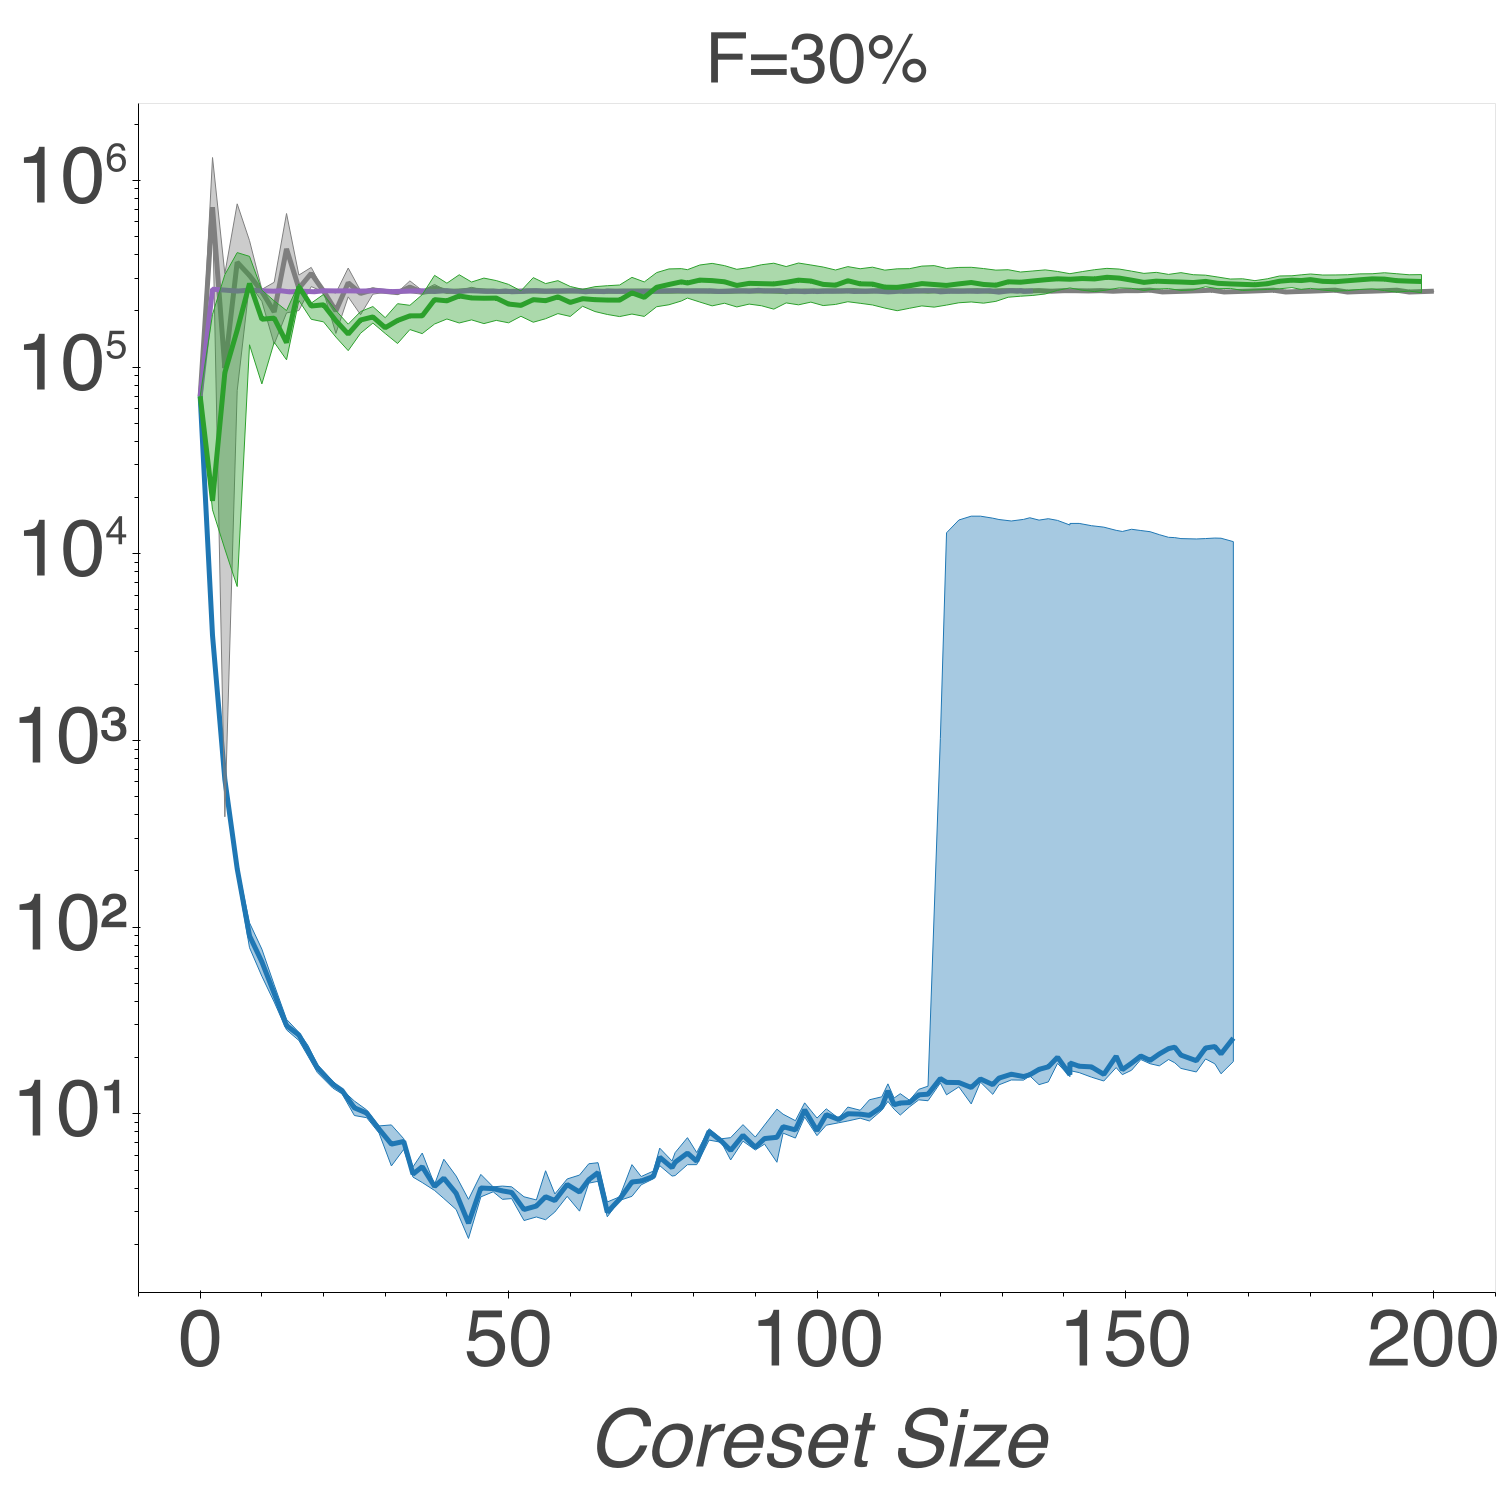
\includegraphics[width=.3\textwidth]{figs/f30KLDvsCstSize.png}
\end{frame}

\begin{frame}
	\frametitle{Gaussian Mean Inference under Stuctured Data Contamination: Effects of varying the robustness hyperparameter}
	\centering
			\centering
	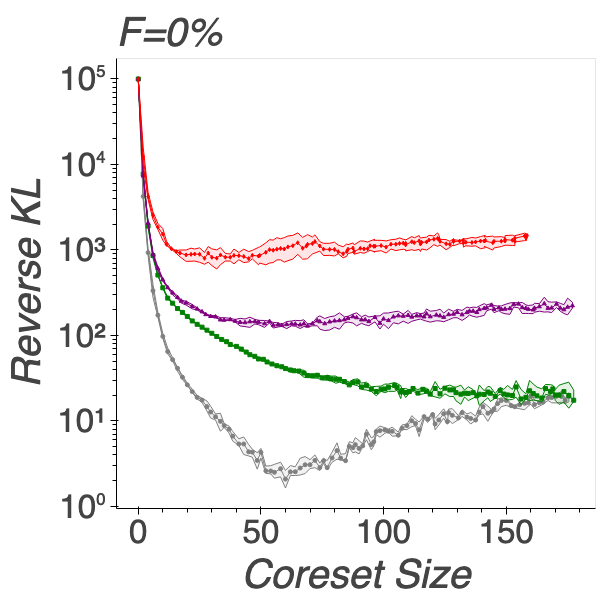
\includegraphics[width=.325\textwidth]{figs/comp_beta_F0_KLDvsCstSize.png}
	\centering
	\hfill
	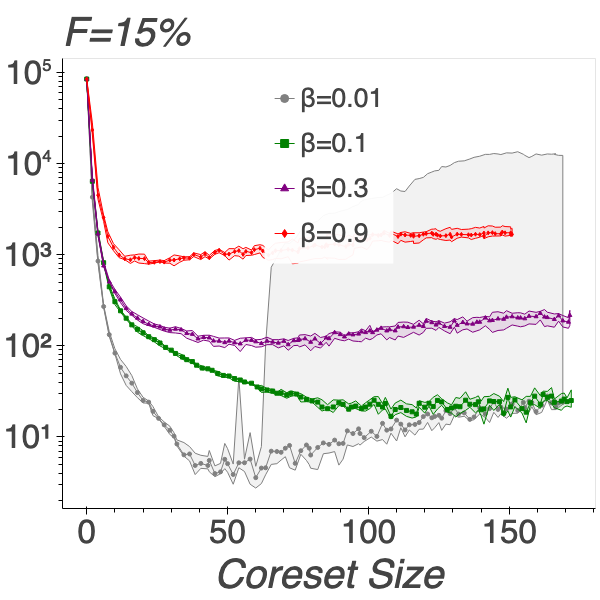
\includegraphics[width=.325\textwidth]{figs/comp_beta_F15_KLDvsCstSize.png}
	\centering
	\hfill
	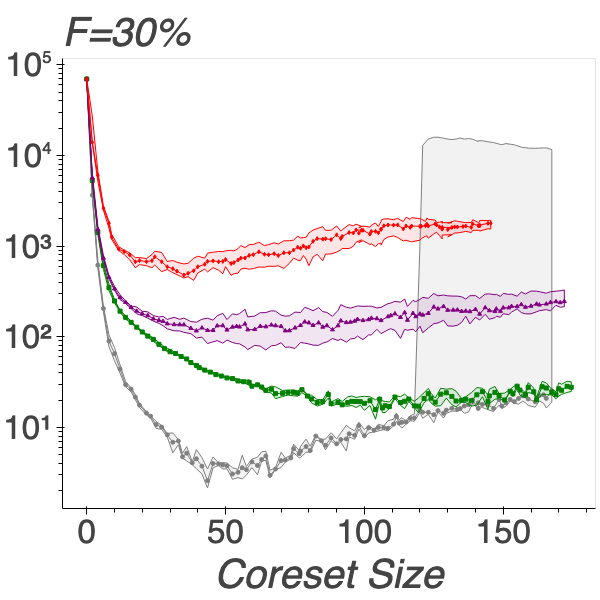
\includegraphics[width=.325\textwidth]{figs/comp_beta_F30_KLDvsCstSize.png}
	\centering

\end{frame}

\begin{frame}
	\frametitle{Experiment II: Bayesian Logistic Regression under Mislabeling and Feature Noise}
	\centering
	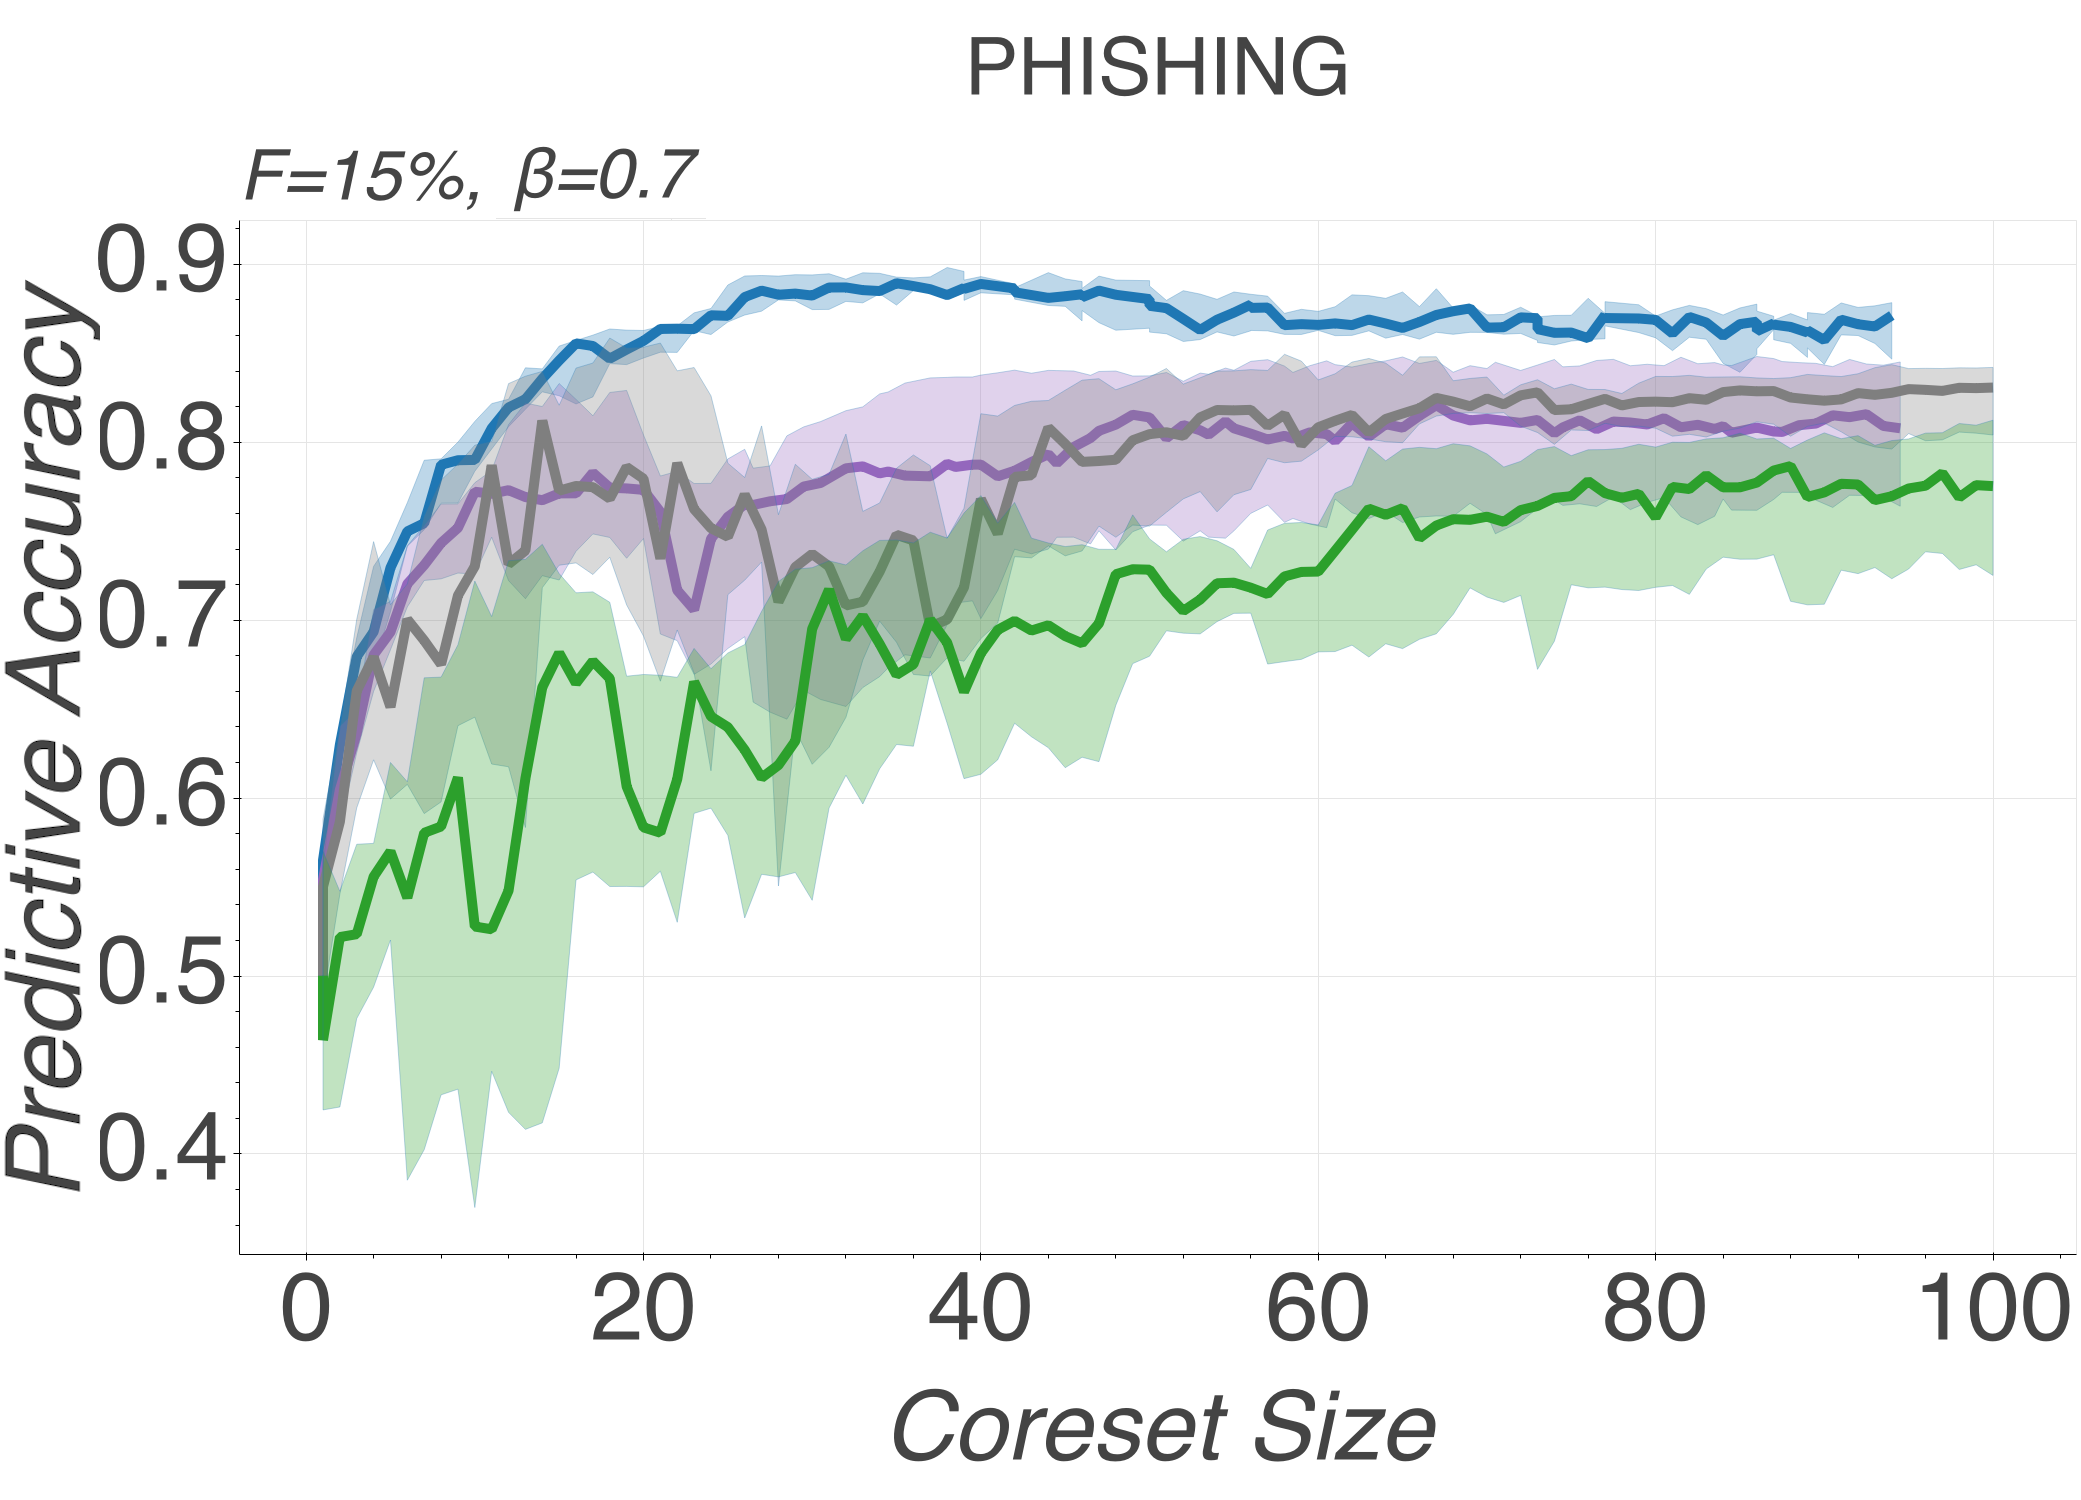
\includegraphics[width=.49\textwidth, height=3.8cm]{figs/phish09_10_15_False_False_ACCvssz.png}
	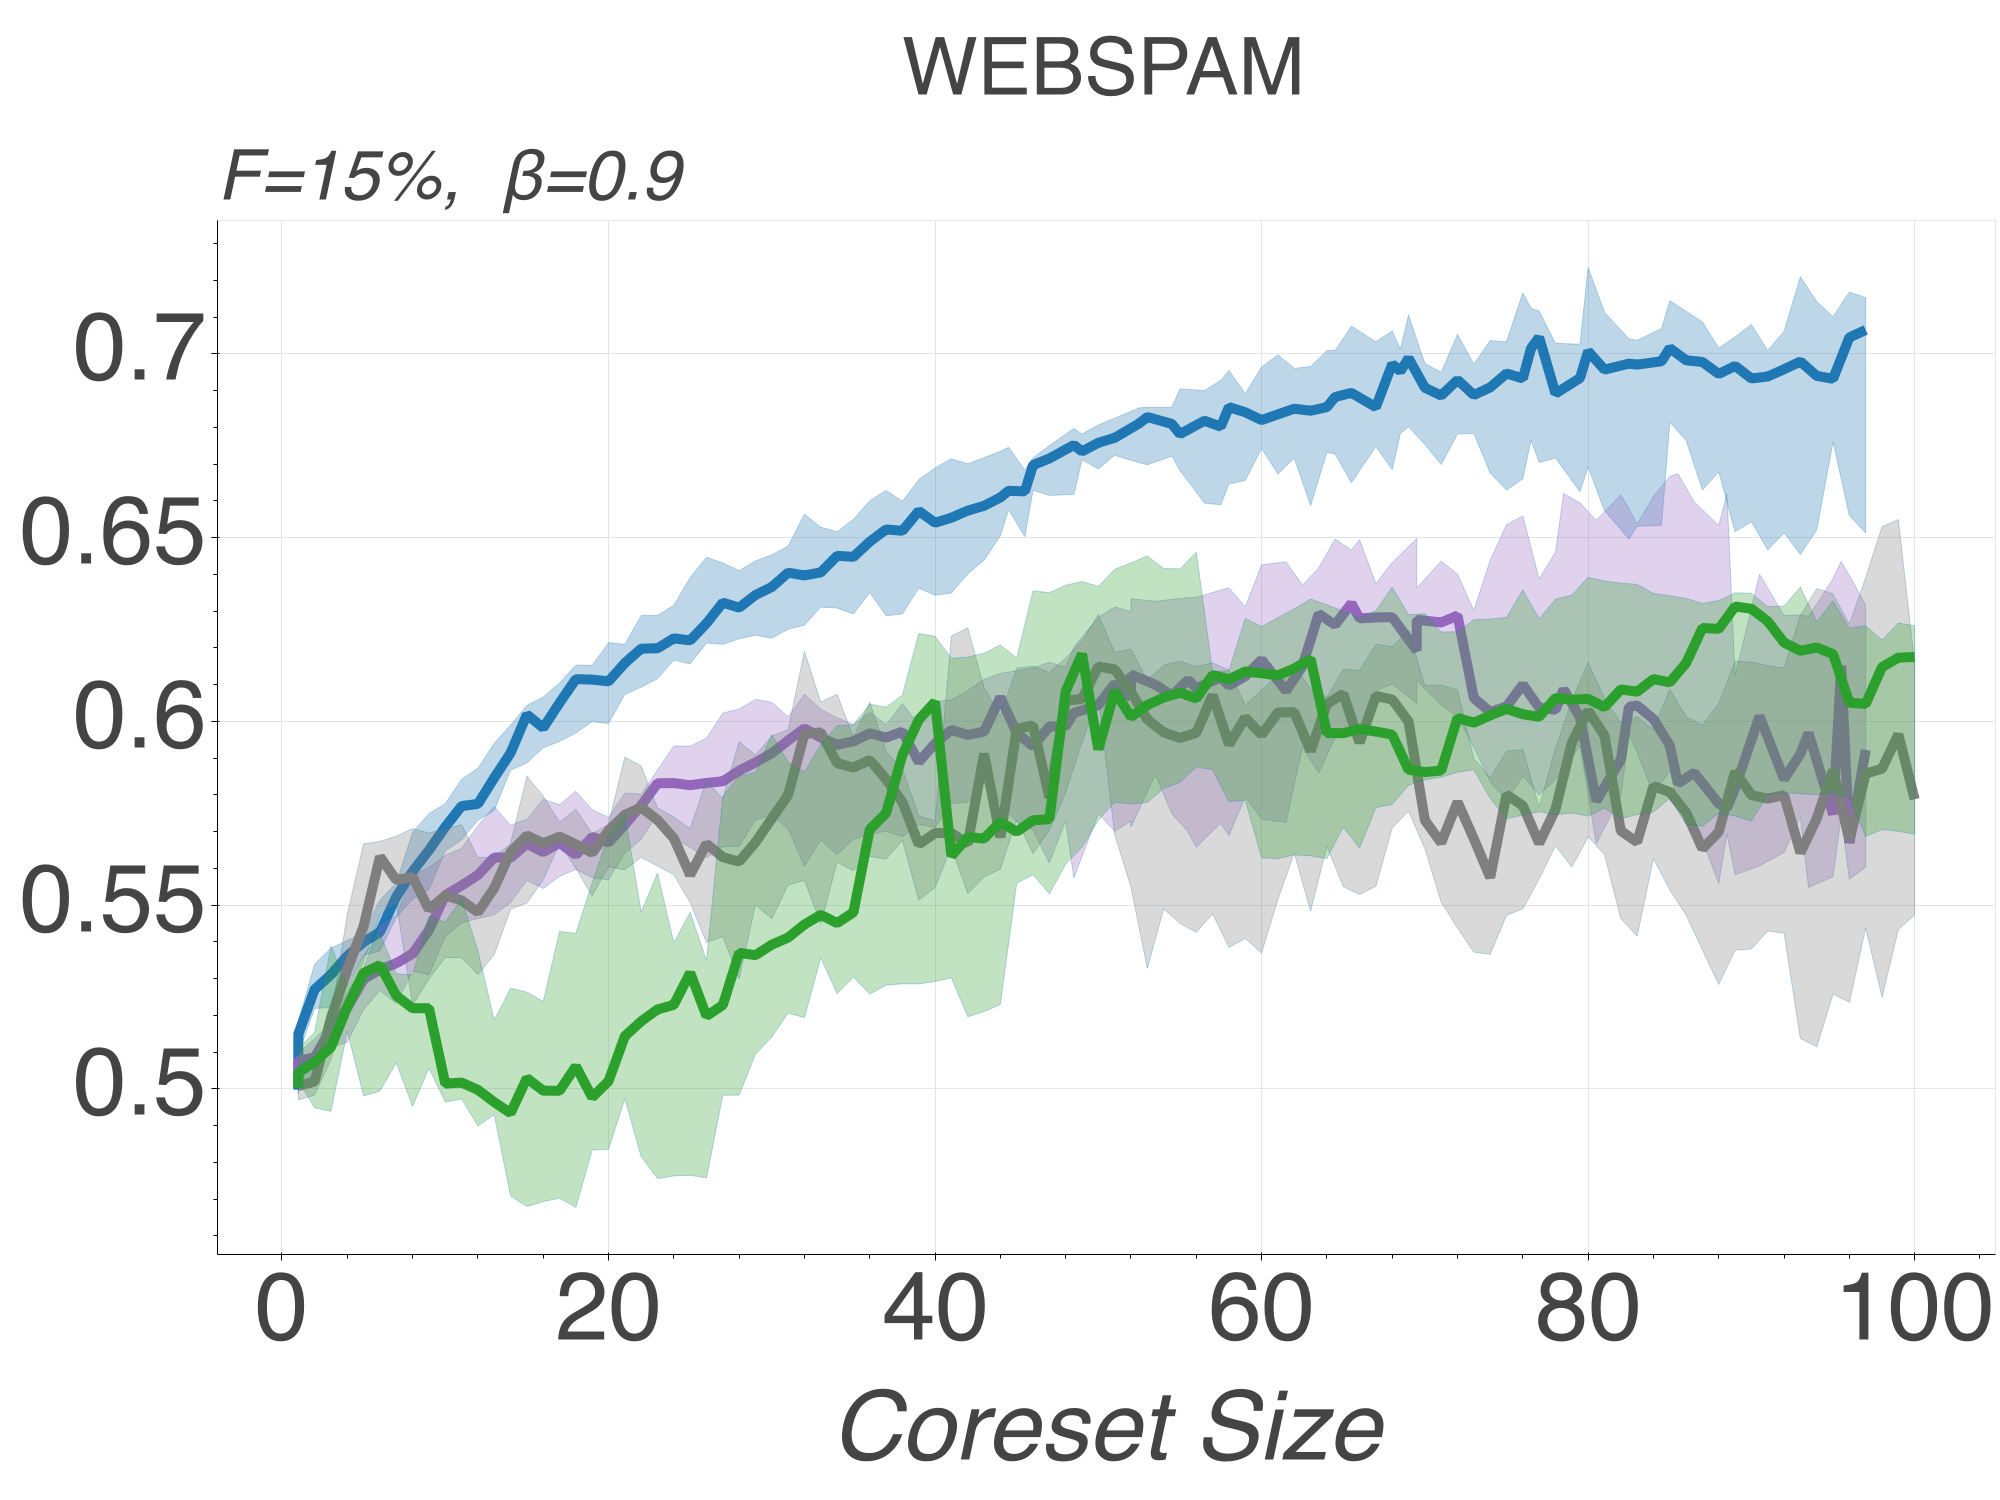
\includegraphics[width=.49\textwidth, height=3.8cm]{figs/webspam09_10_15_True_False_ACCvssz.png}
	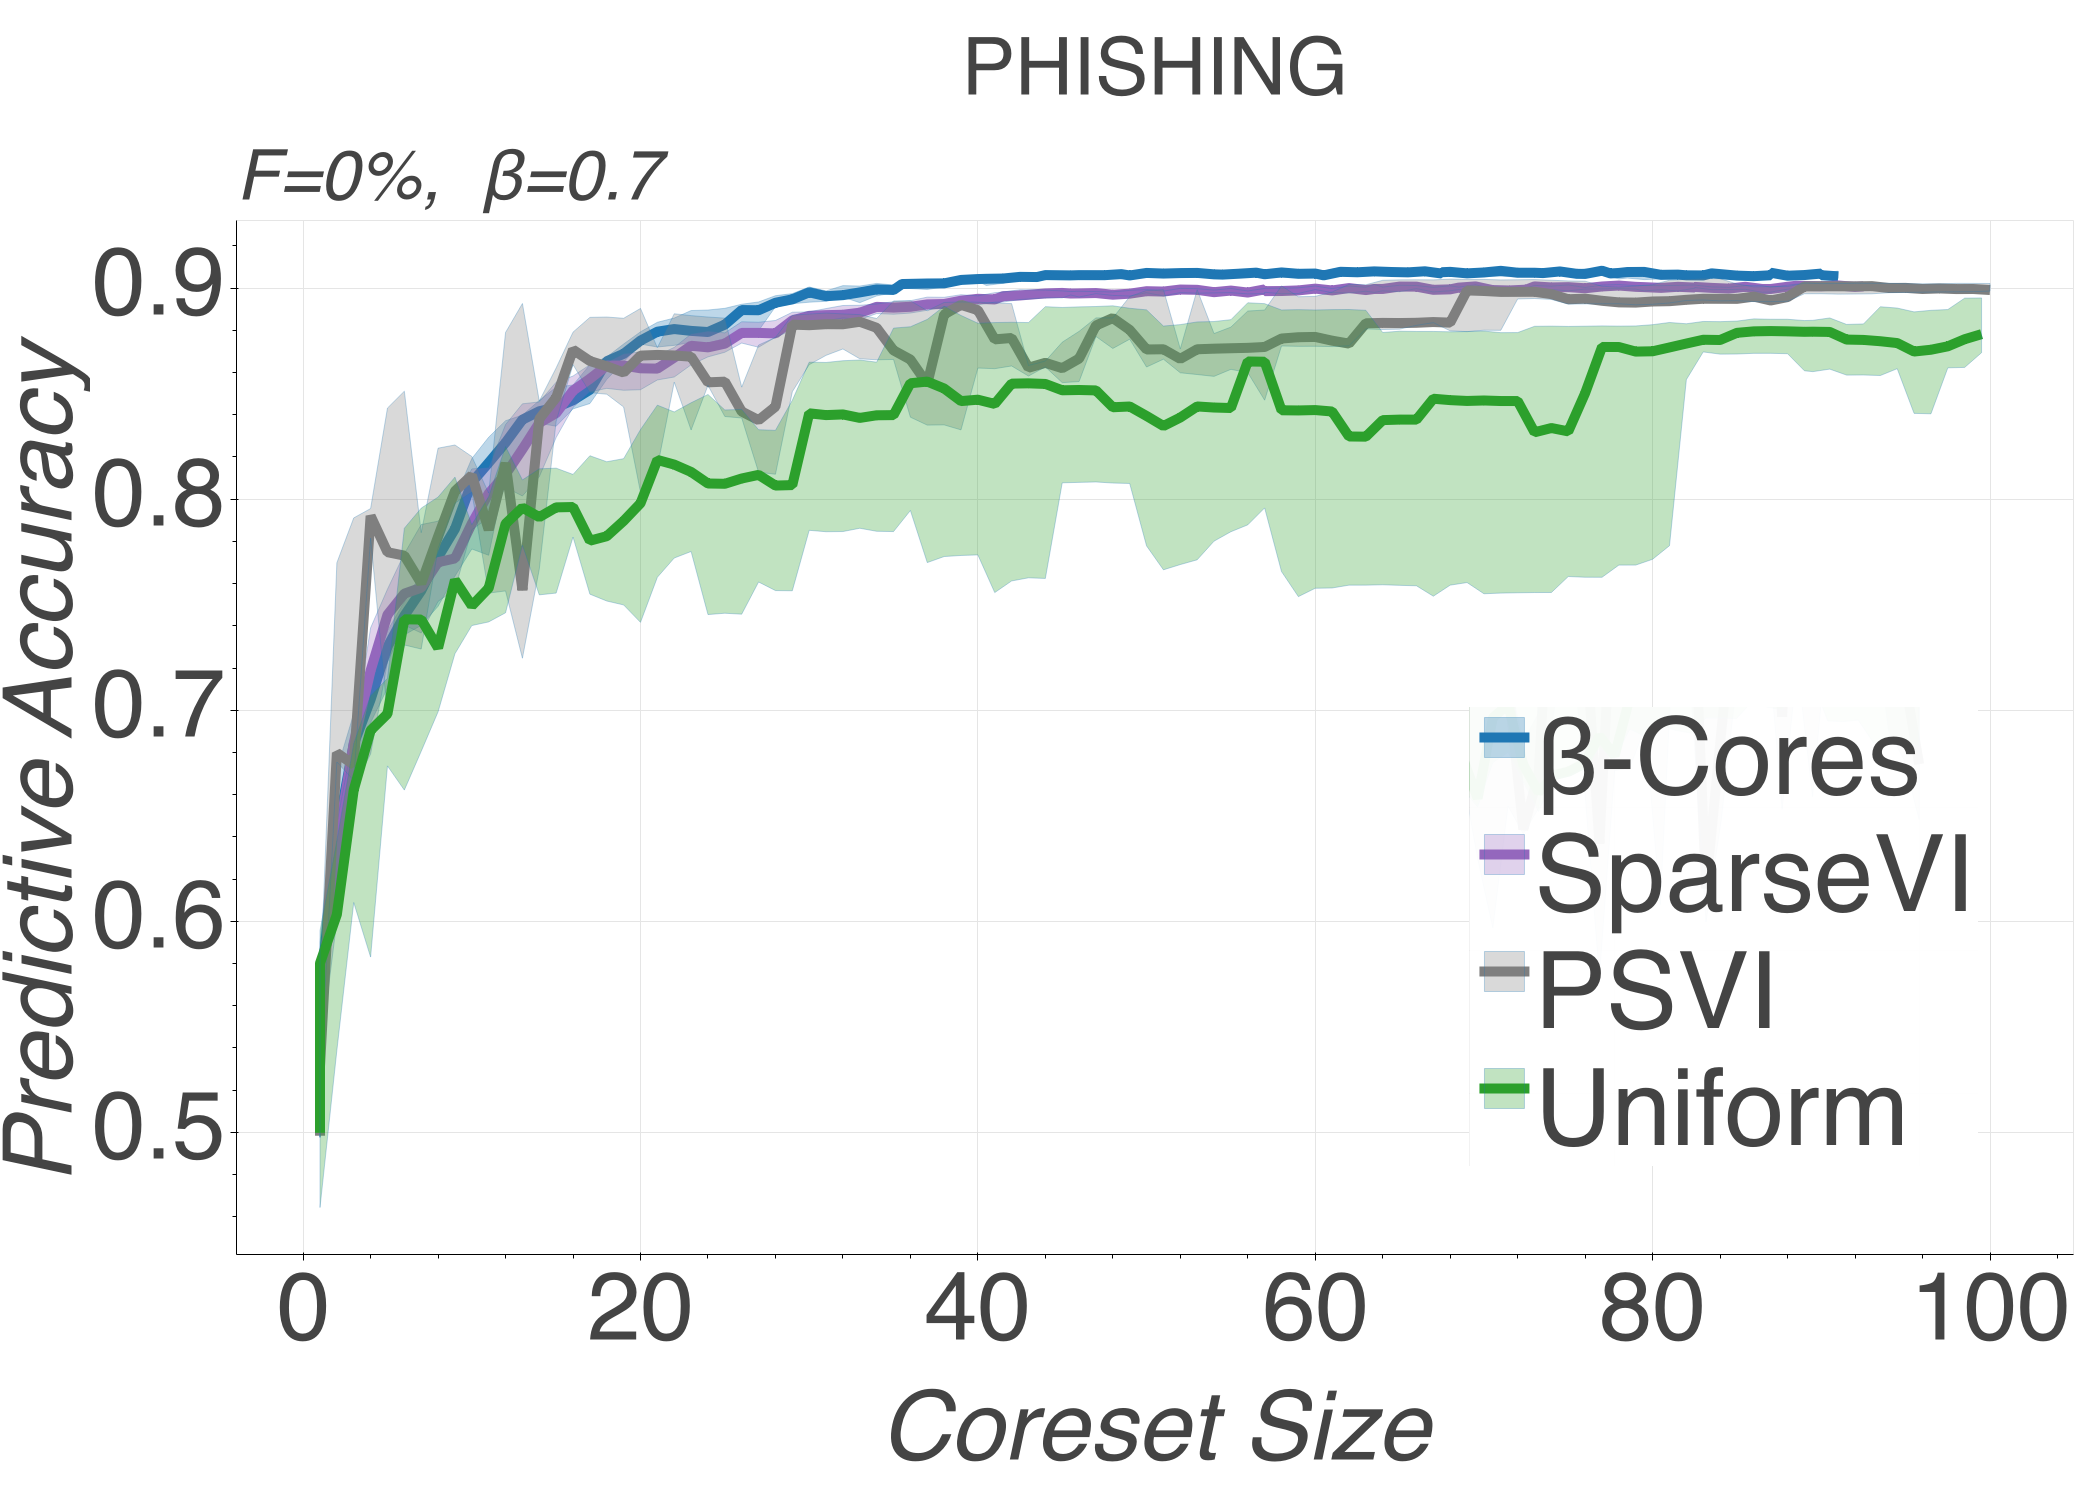
\includegraphics[width=.49\textwidth, height=3.8cm]{figs/phish07_10_0_False_False_ACCvssz.png}
	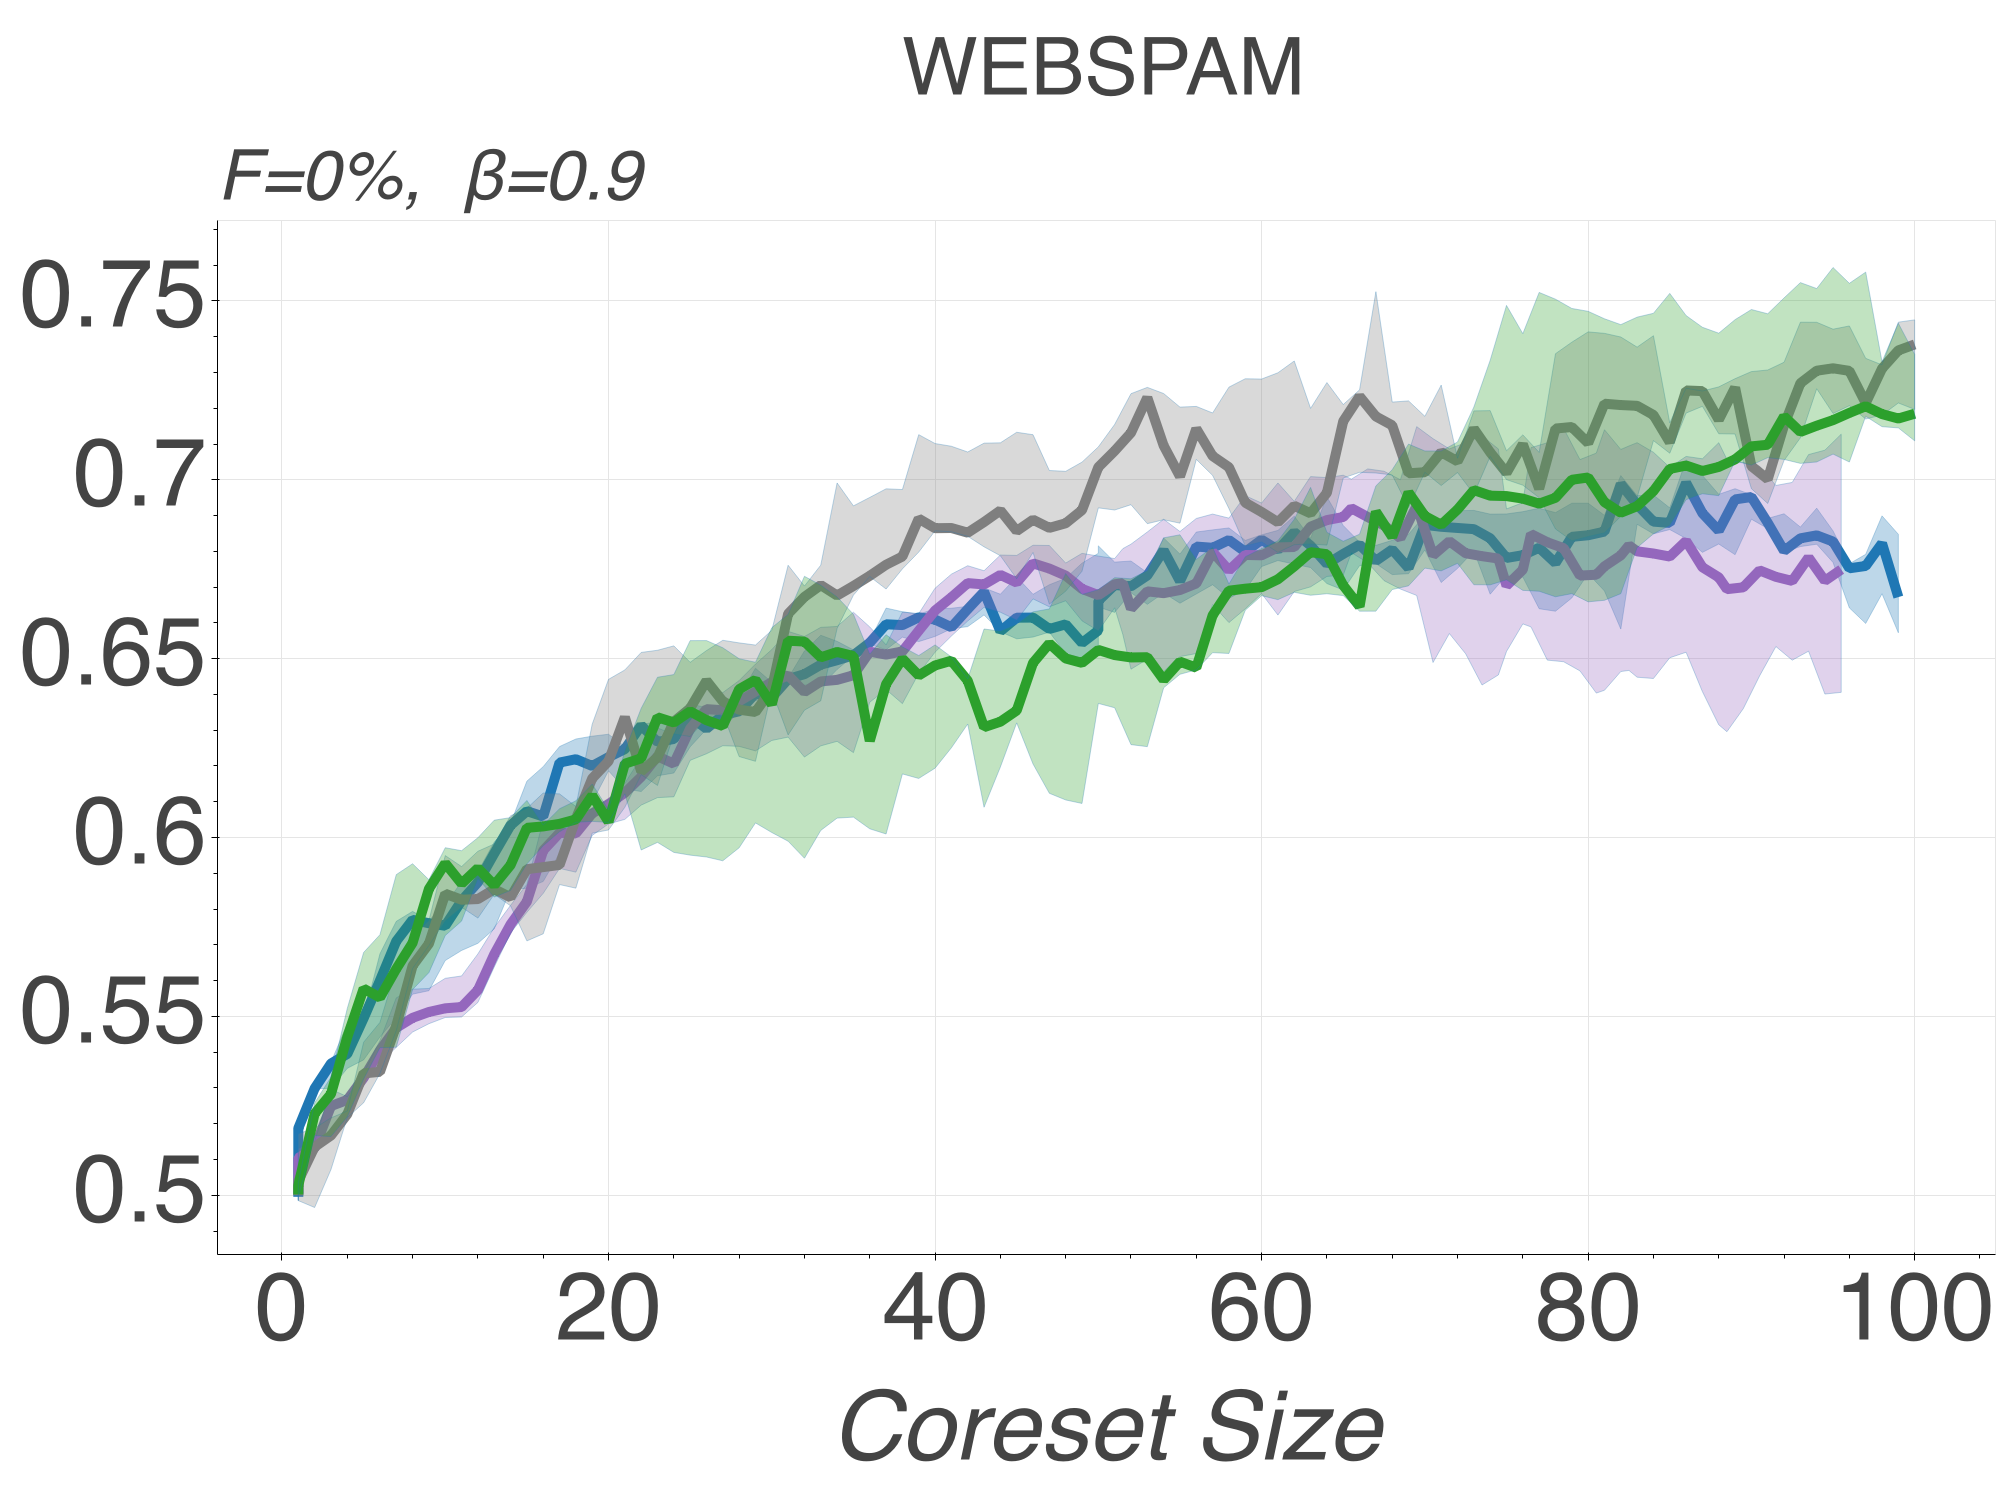
\includegraphics[width=.49\textwidth, height=3.8cm]{figs/webspam09_10_0_True_False_ACCvssz.png}
\end{frame}

\begin{frame}
	\frametitle{Experiment III: Neural Linear Regression on Noisy Data Batches}
	\centering
	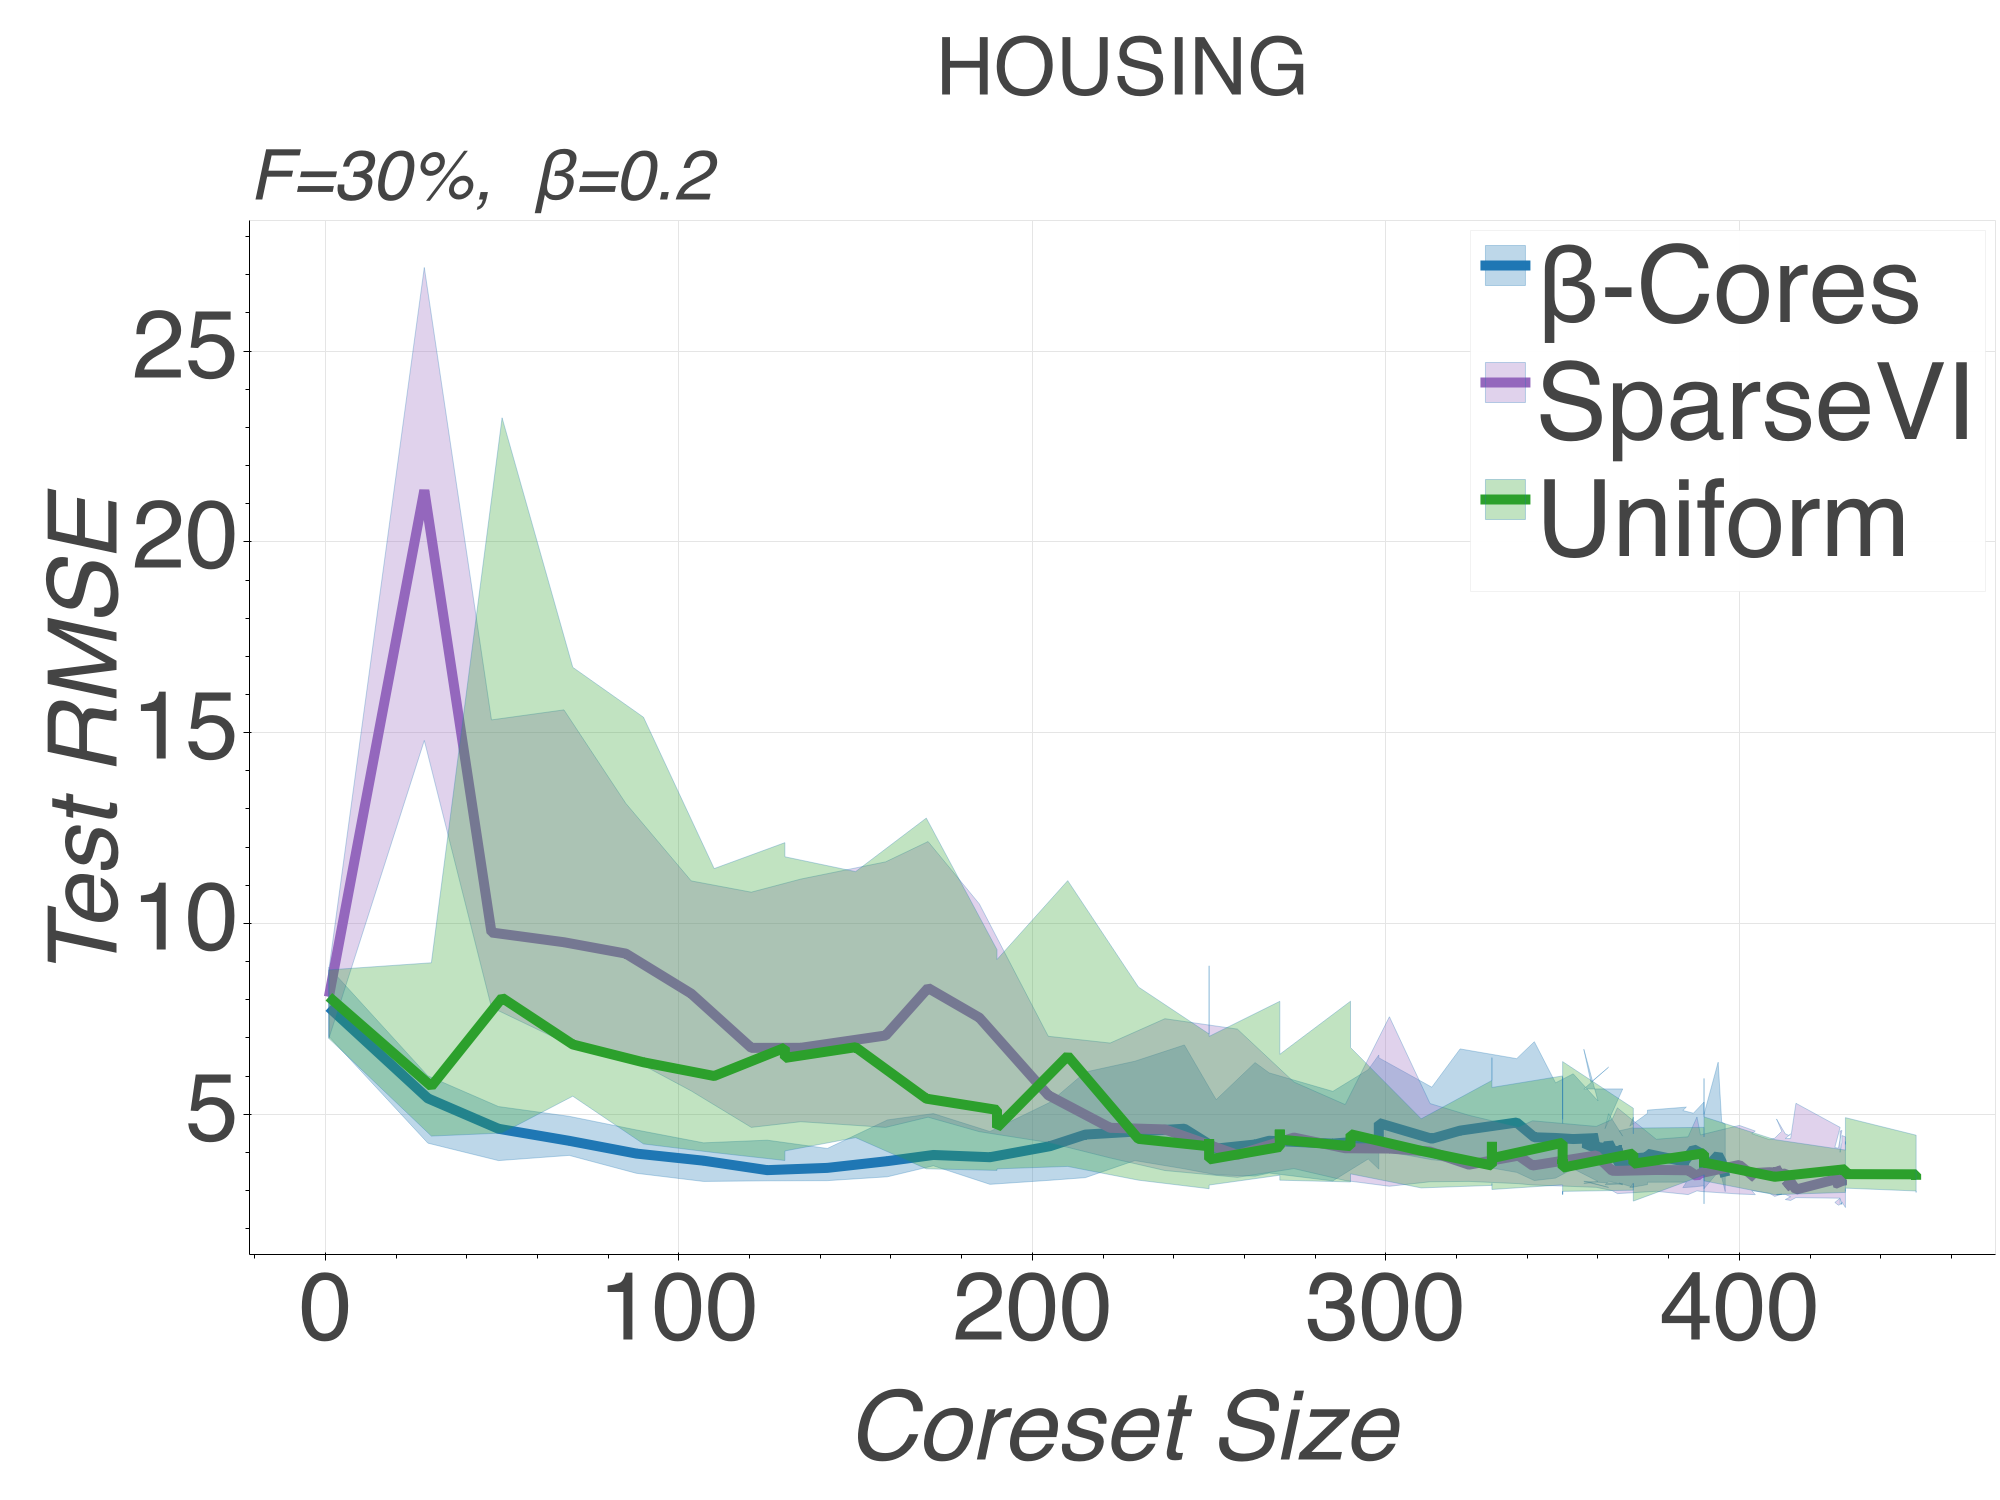
\includegraphics[width=.49\textwidth, height=3.8cm]{figs/boston02_01_30_RMSEvssz.png}
	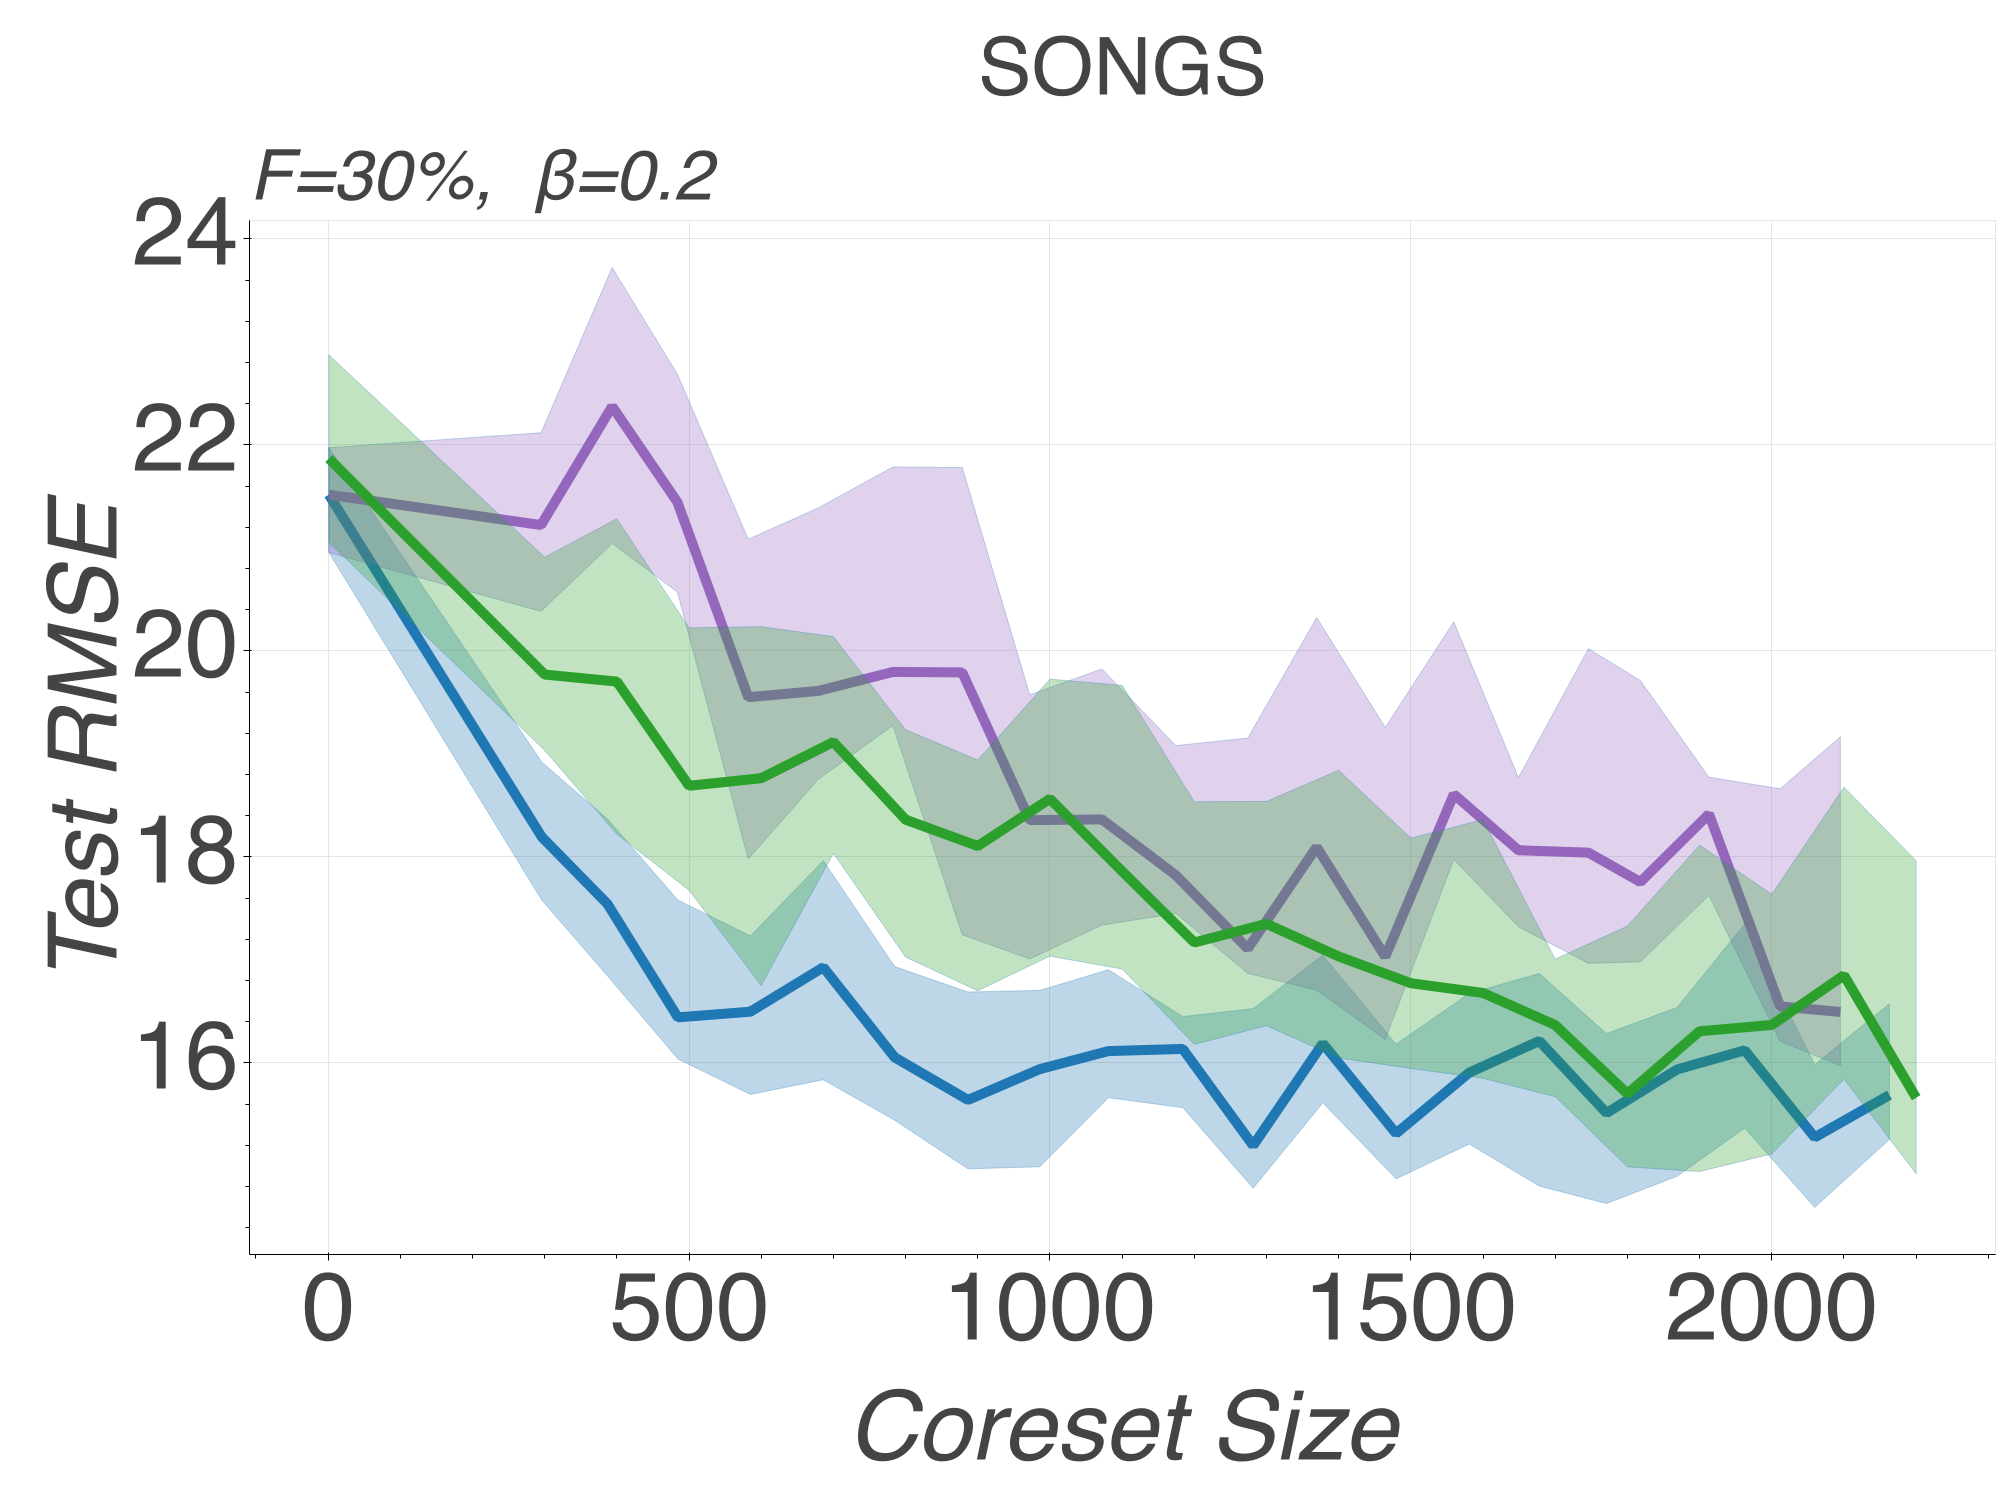
\includegraphics[width=.49\textwidth, height=3.8cm]{figs/year02_01_30_RMSEvssz.png}
	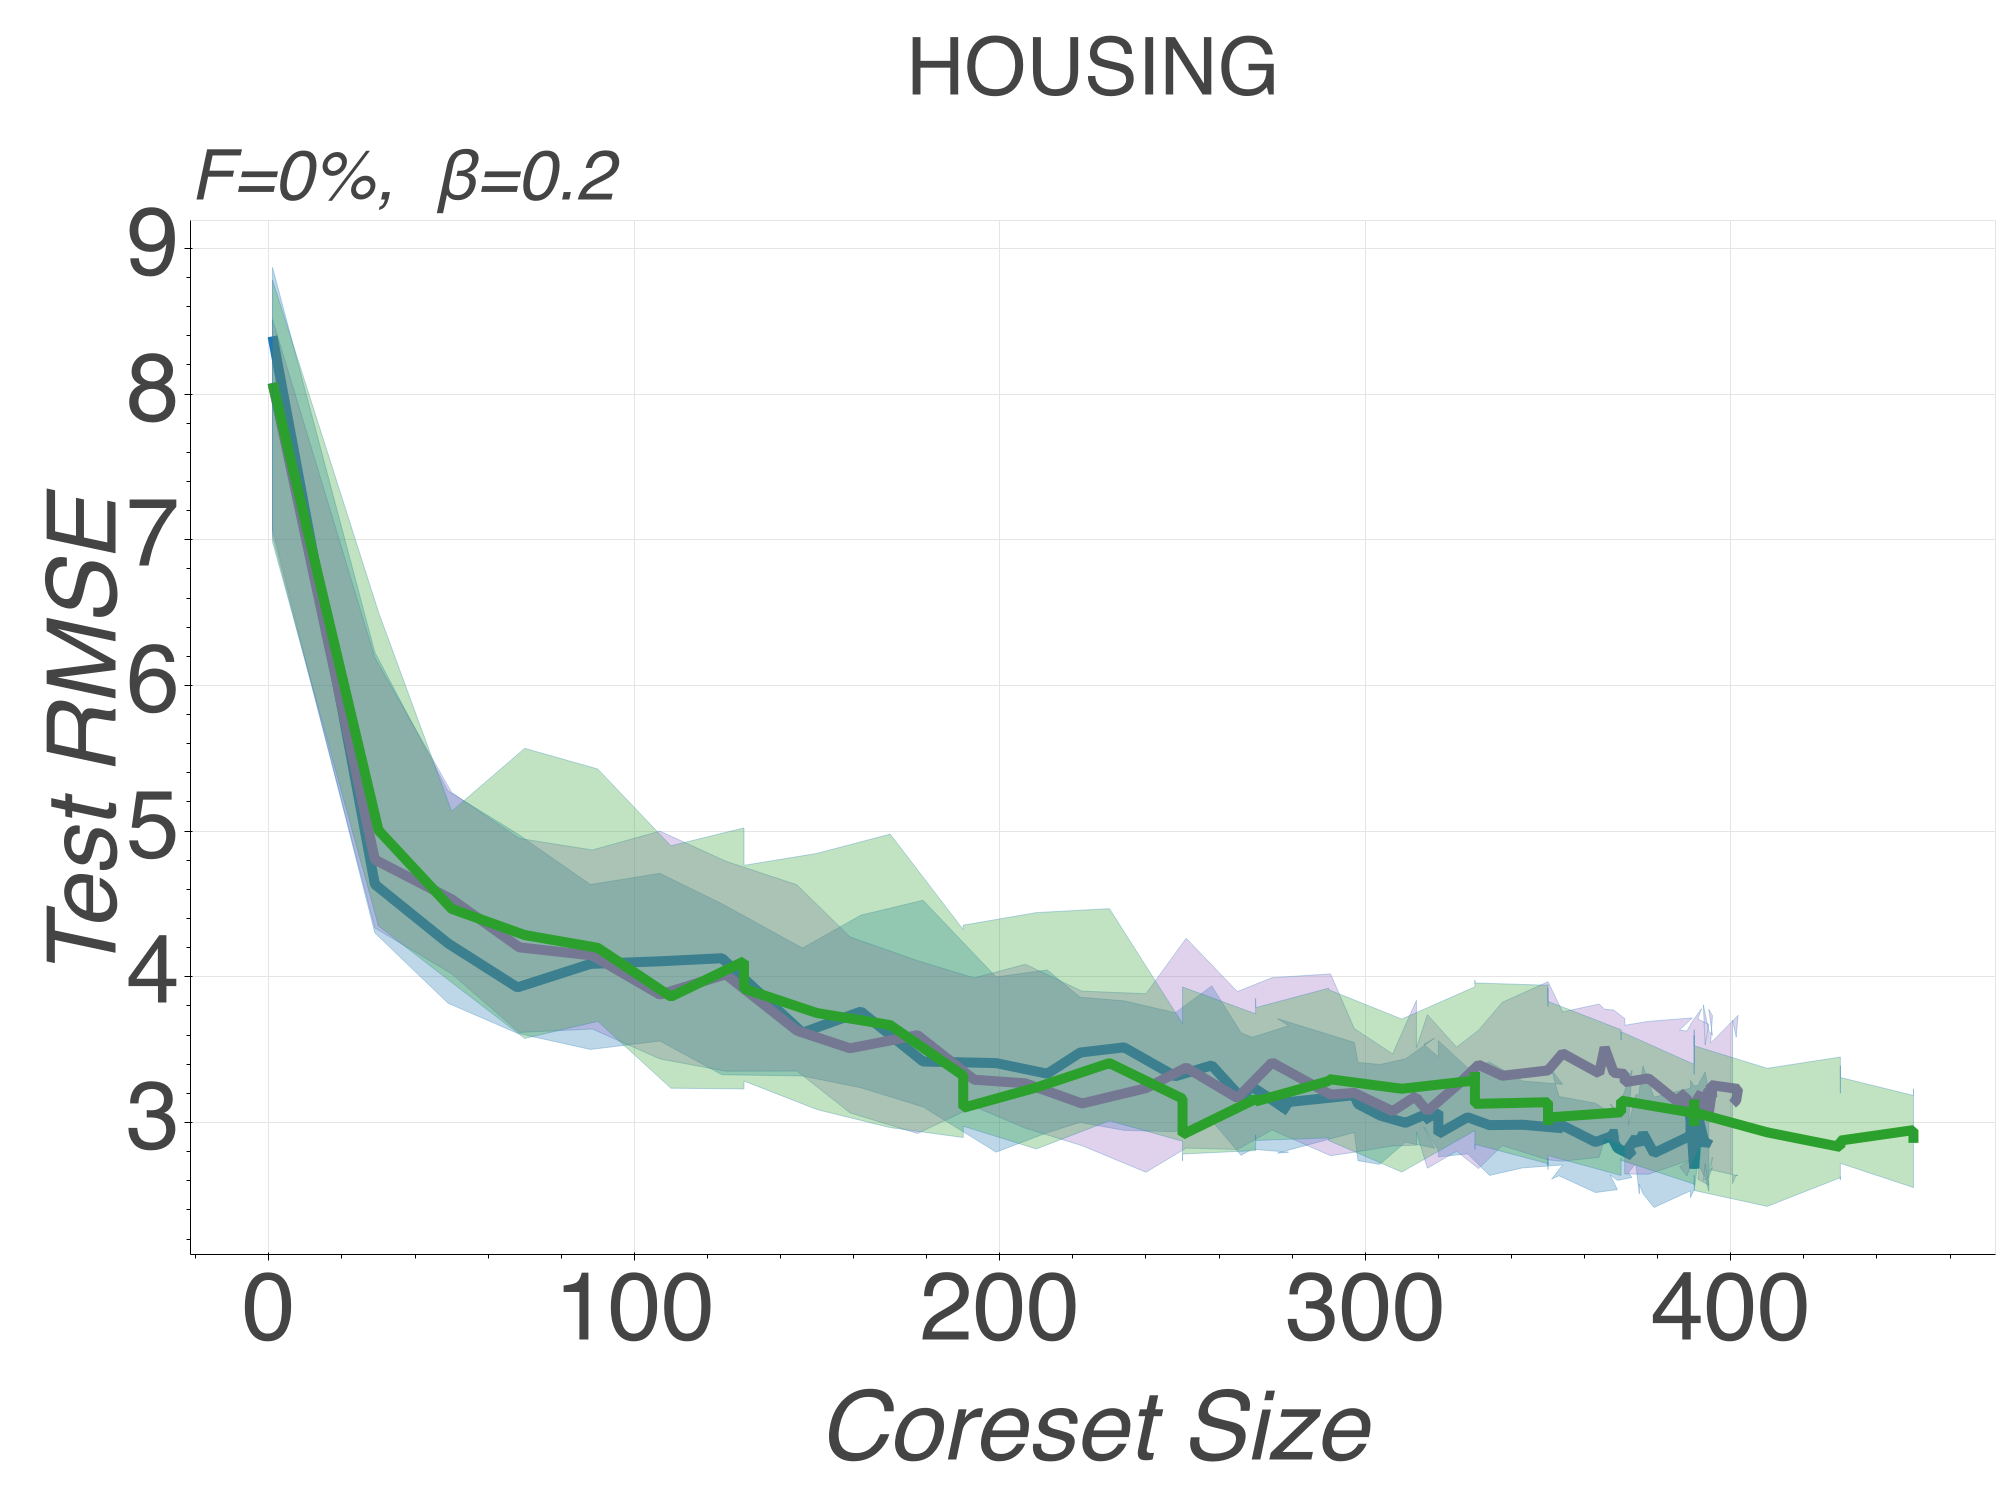
\includegraphics[width=.49\textwidth, height=3.8cm]{figs/boston02_01_0_RMSEvssz.png}
	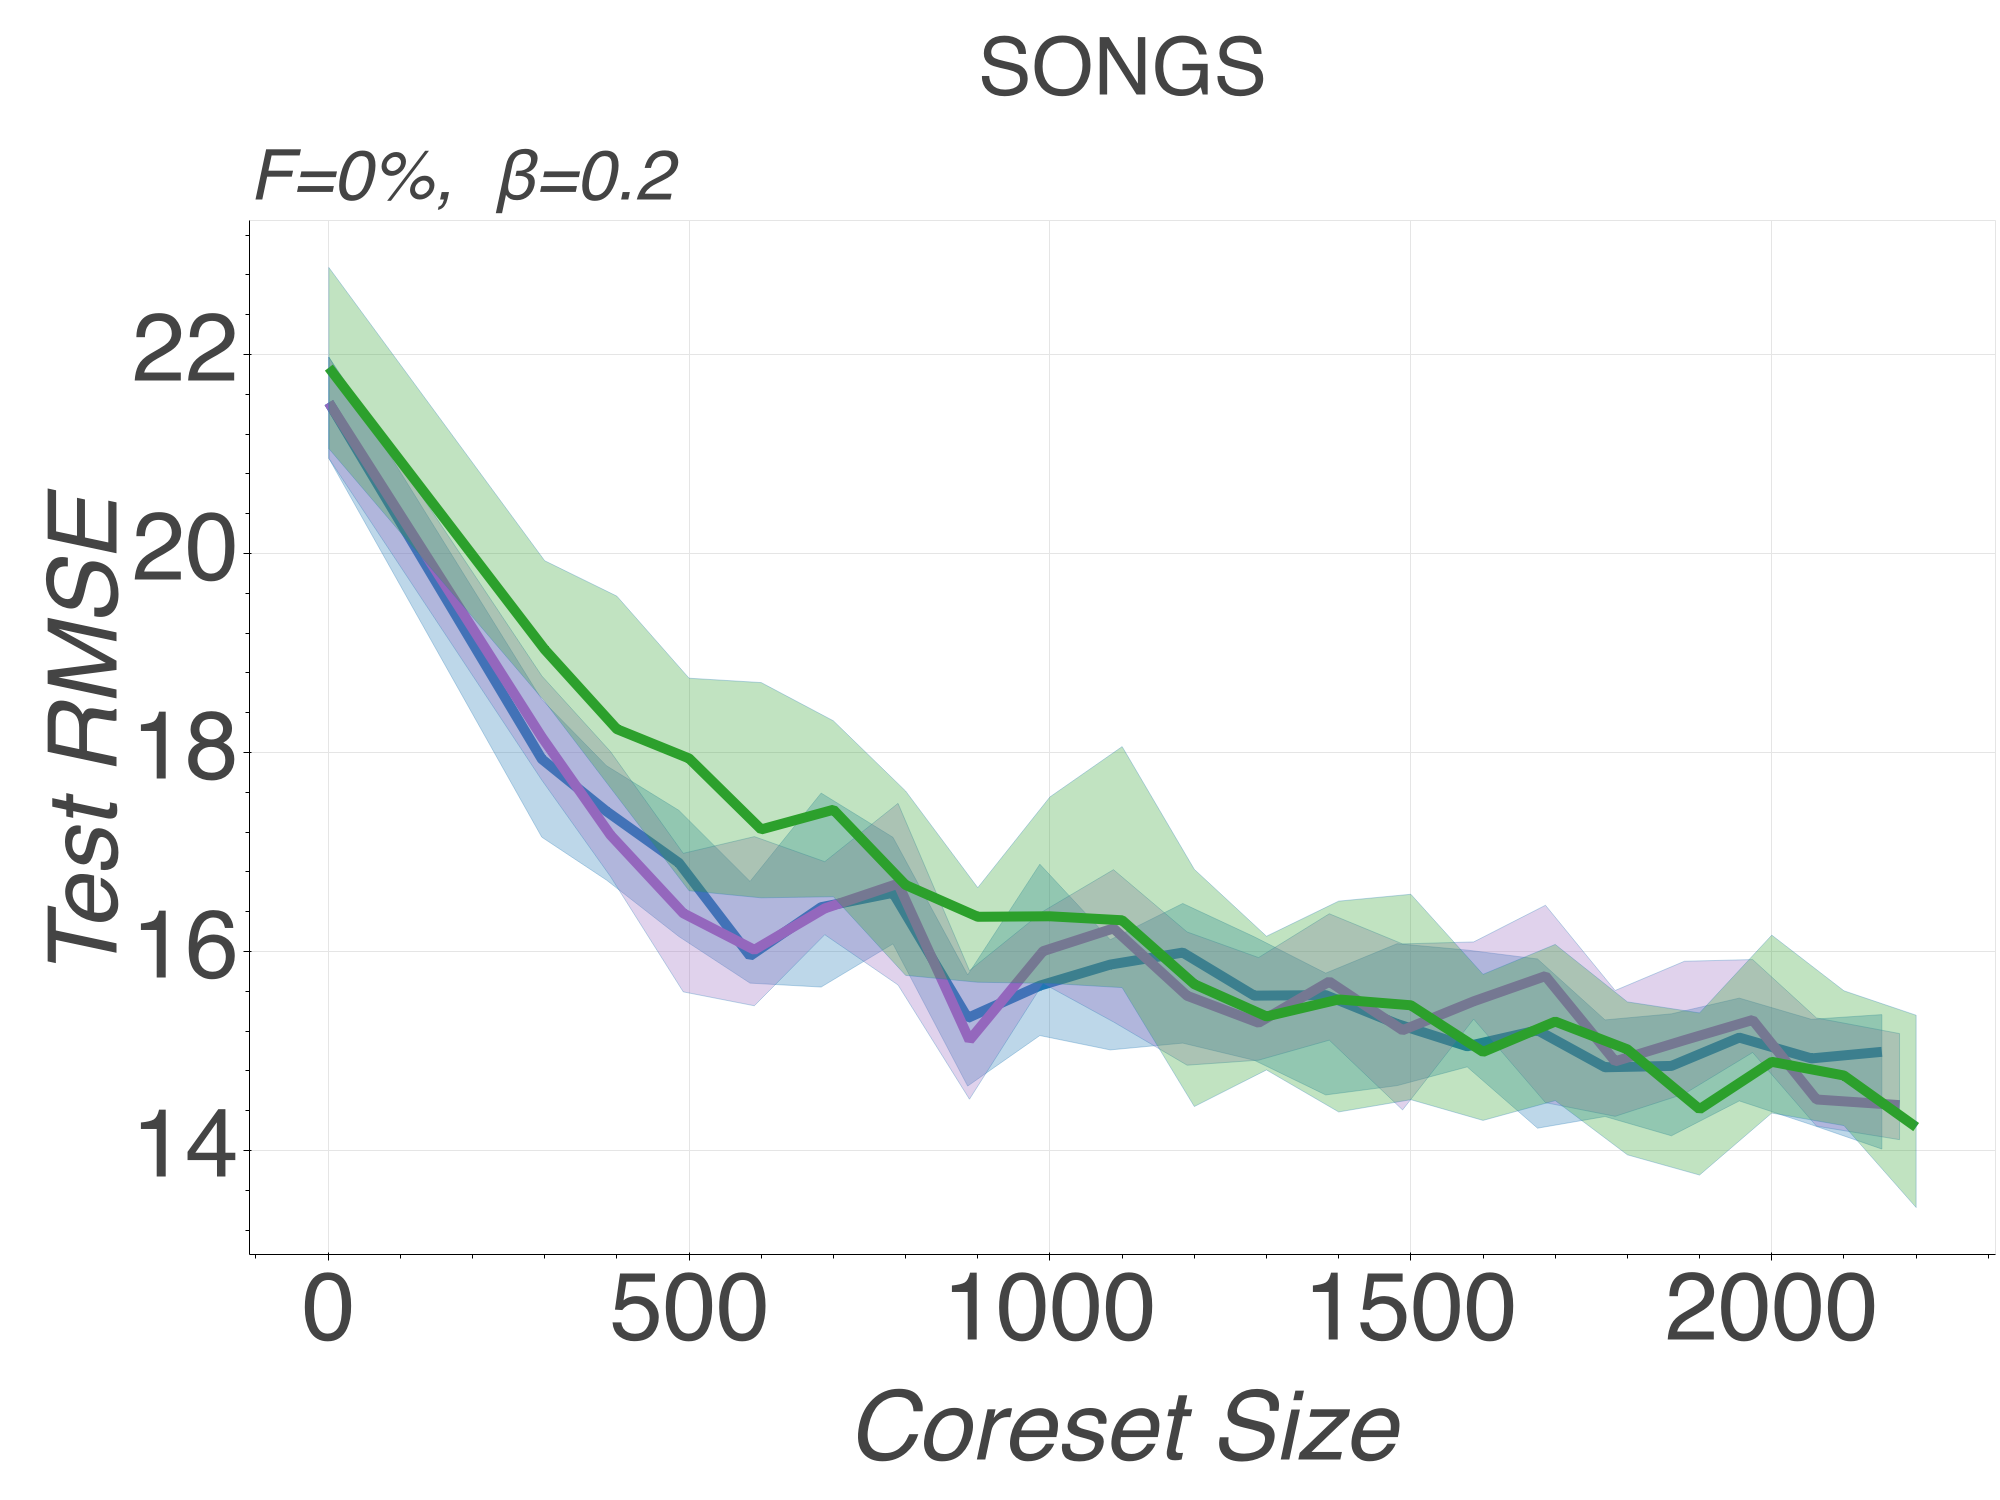
\includegraphics[width=.49\textwidth, height=3.8cm]{figs/year02_01_0_RMSEvssz.png}
\end{frame}

\begin{frame}
	\frametitle{Experiment IV:  Subpopulations Selection for Budgeted Inference on Hospital Readmissions}
	\centering
	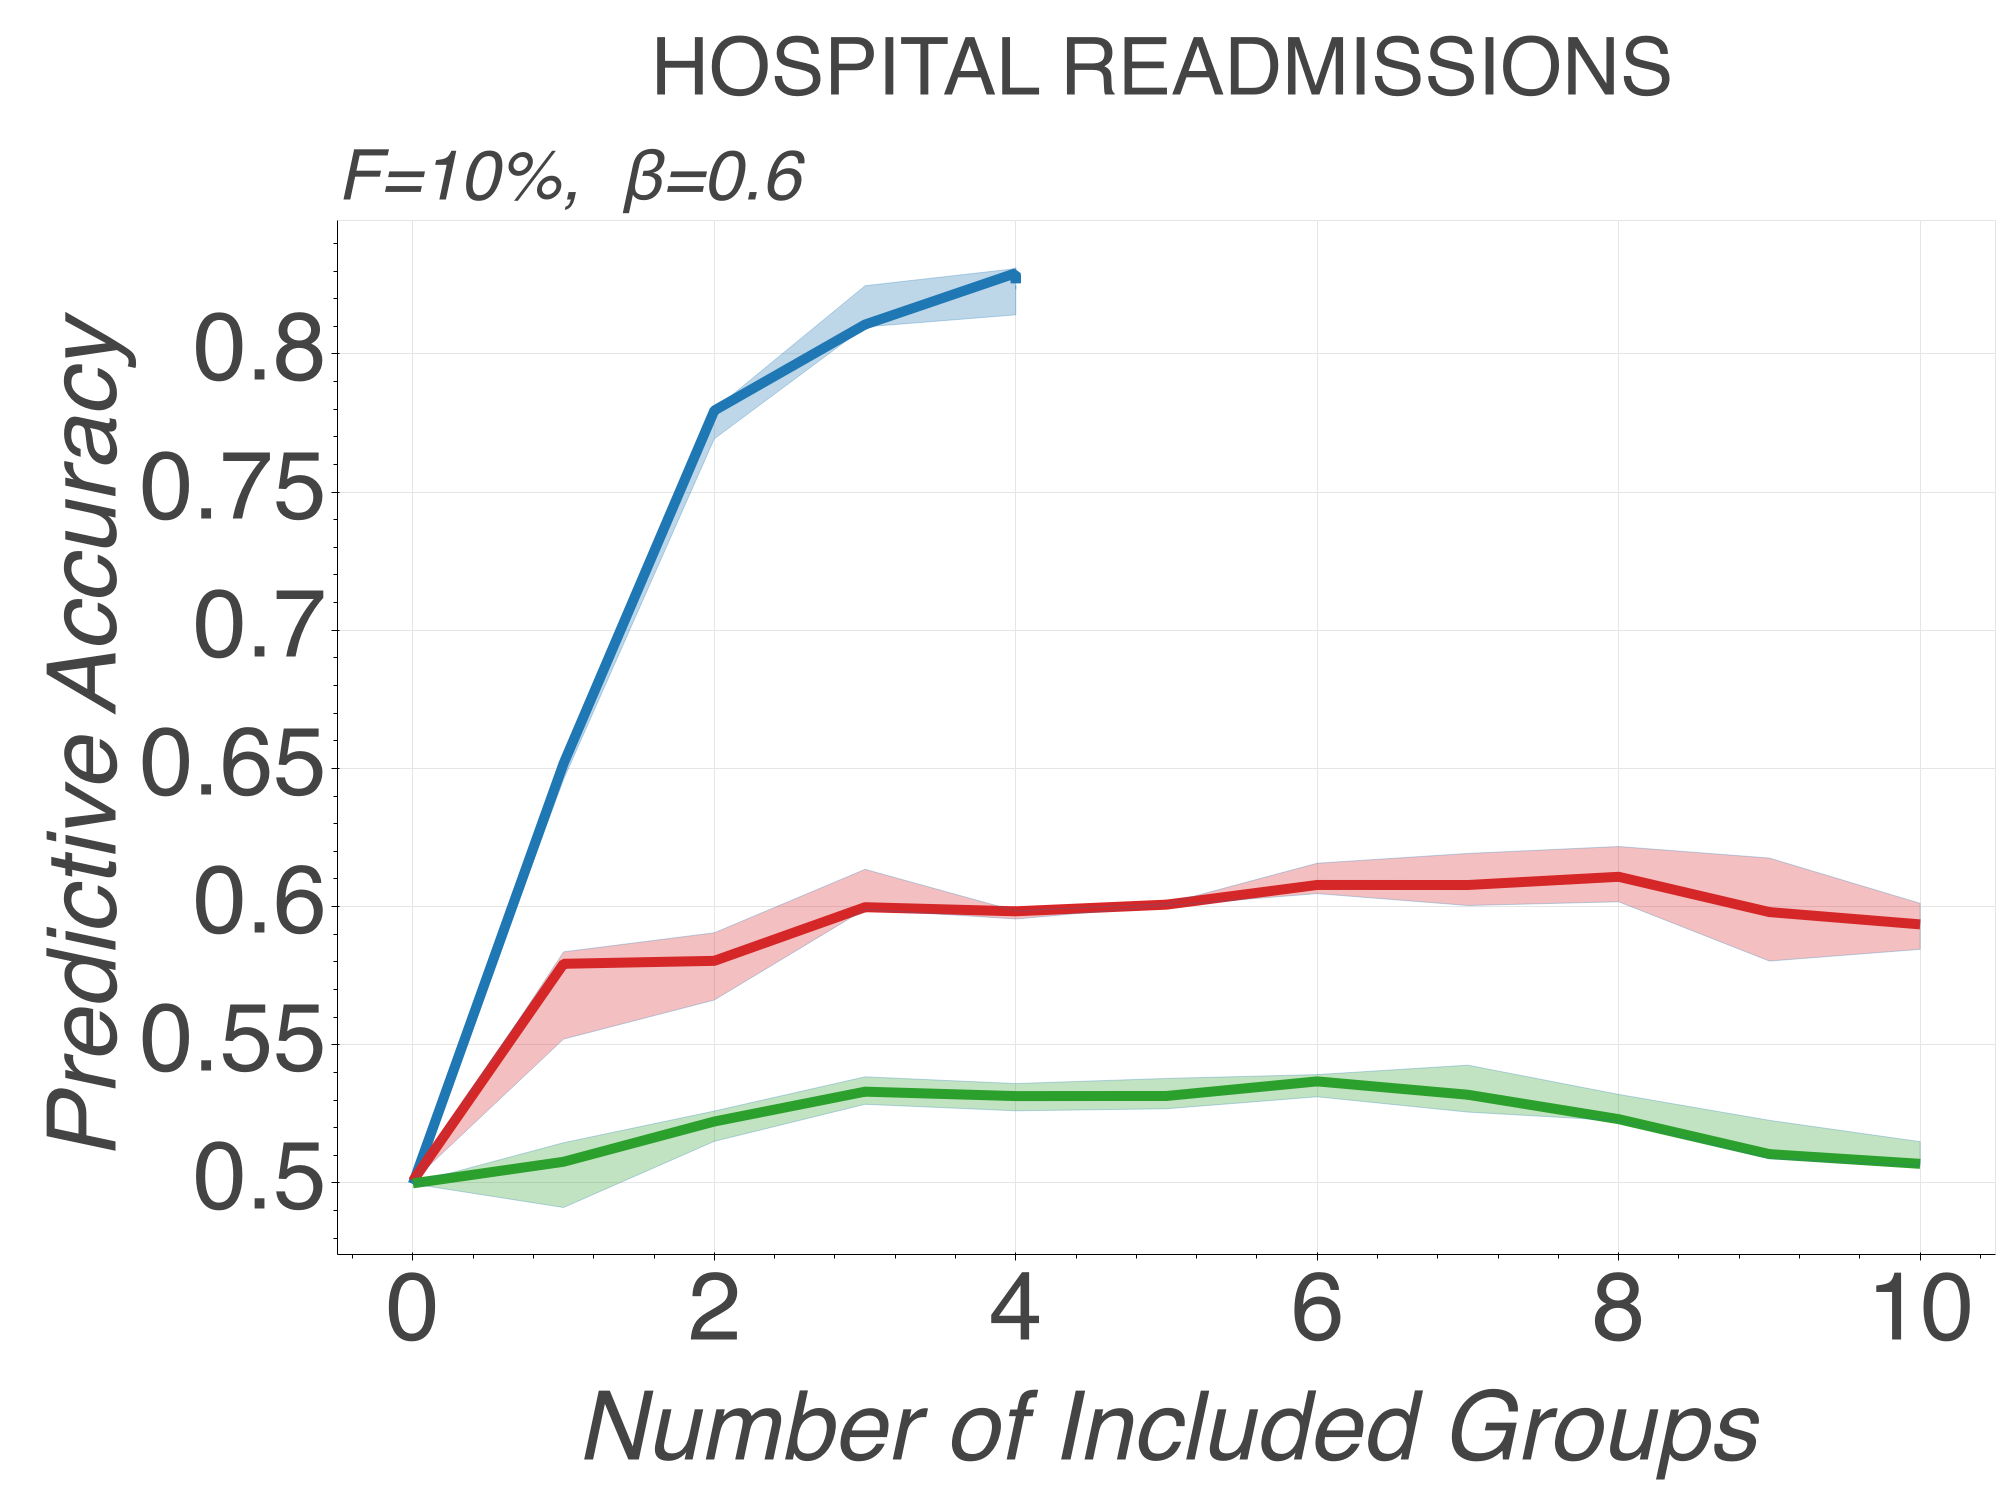
\includegraphics[width=.49\textwidth, height=3.8cm]{figs/group_diabetes06_10_01_False_ACCvsit.png}
	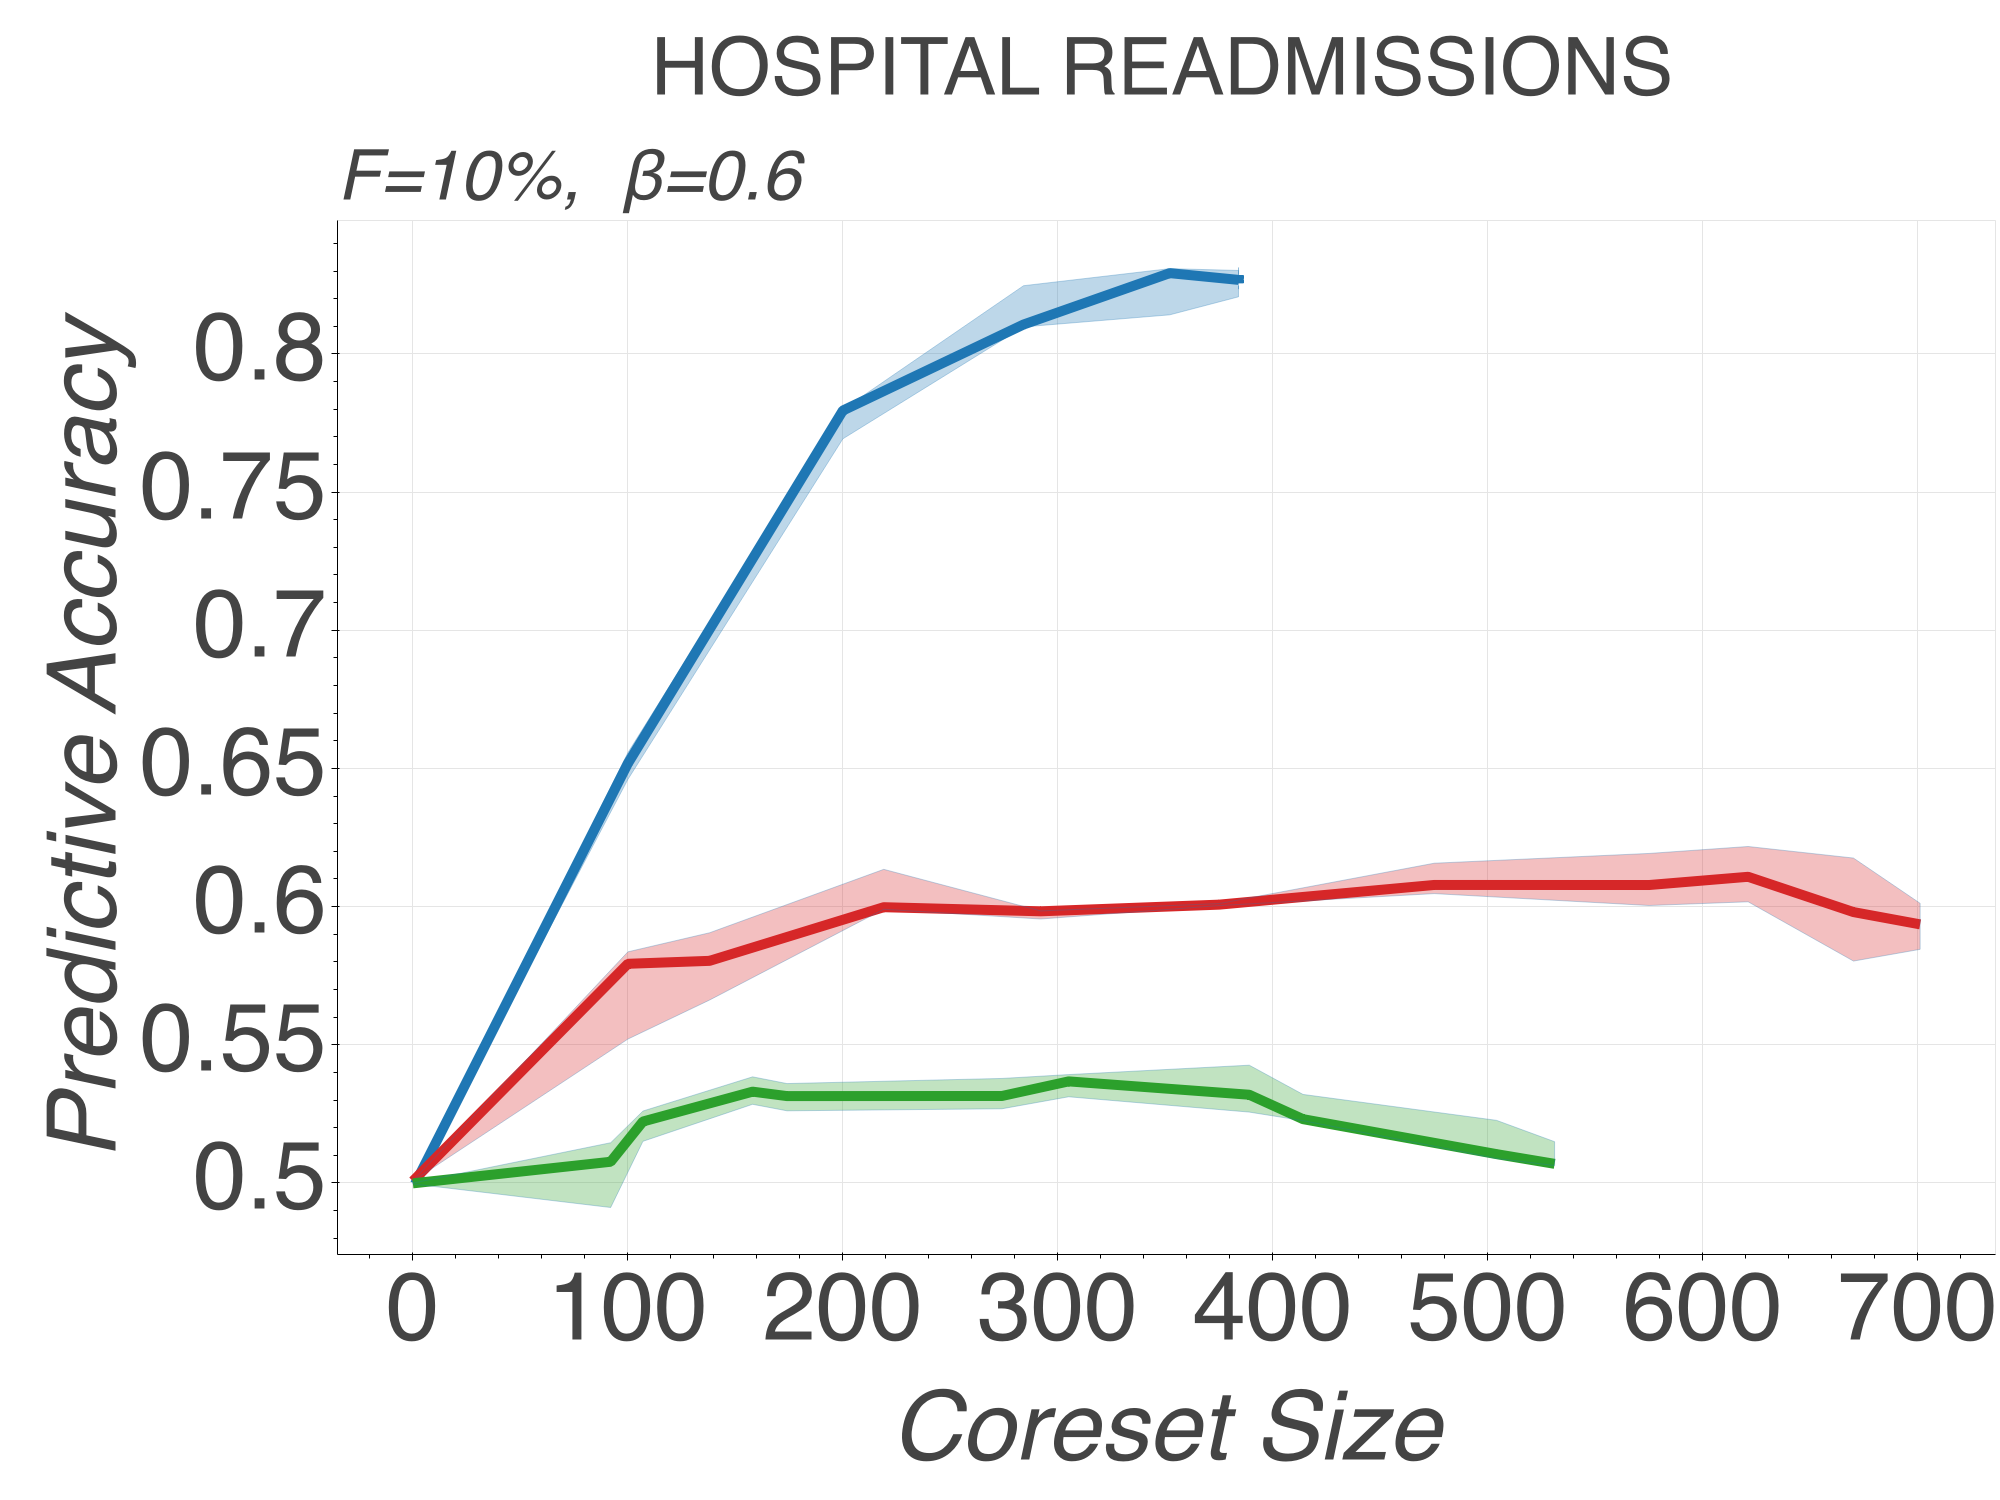
\includegraphics[width=.49\textwidth, height=3.8cm]{figs/group_diabetes06_10_01_False_ACCvssz.png}
	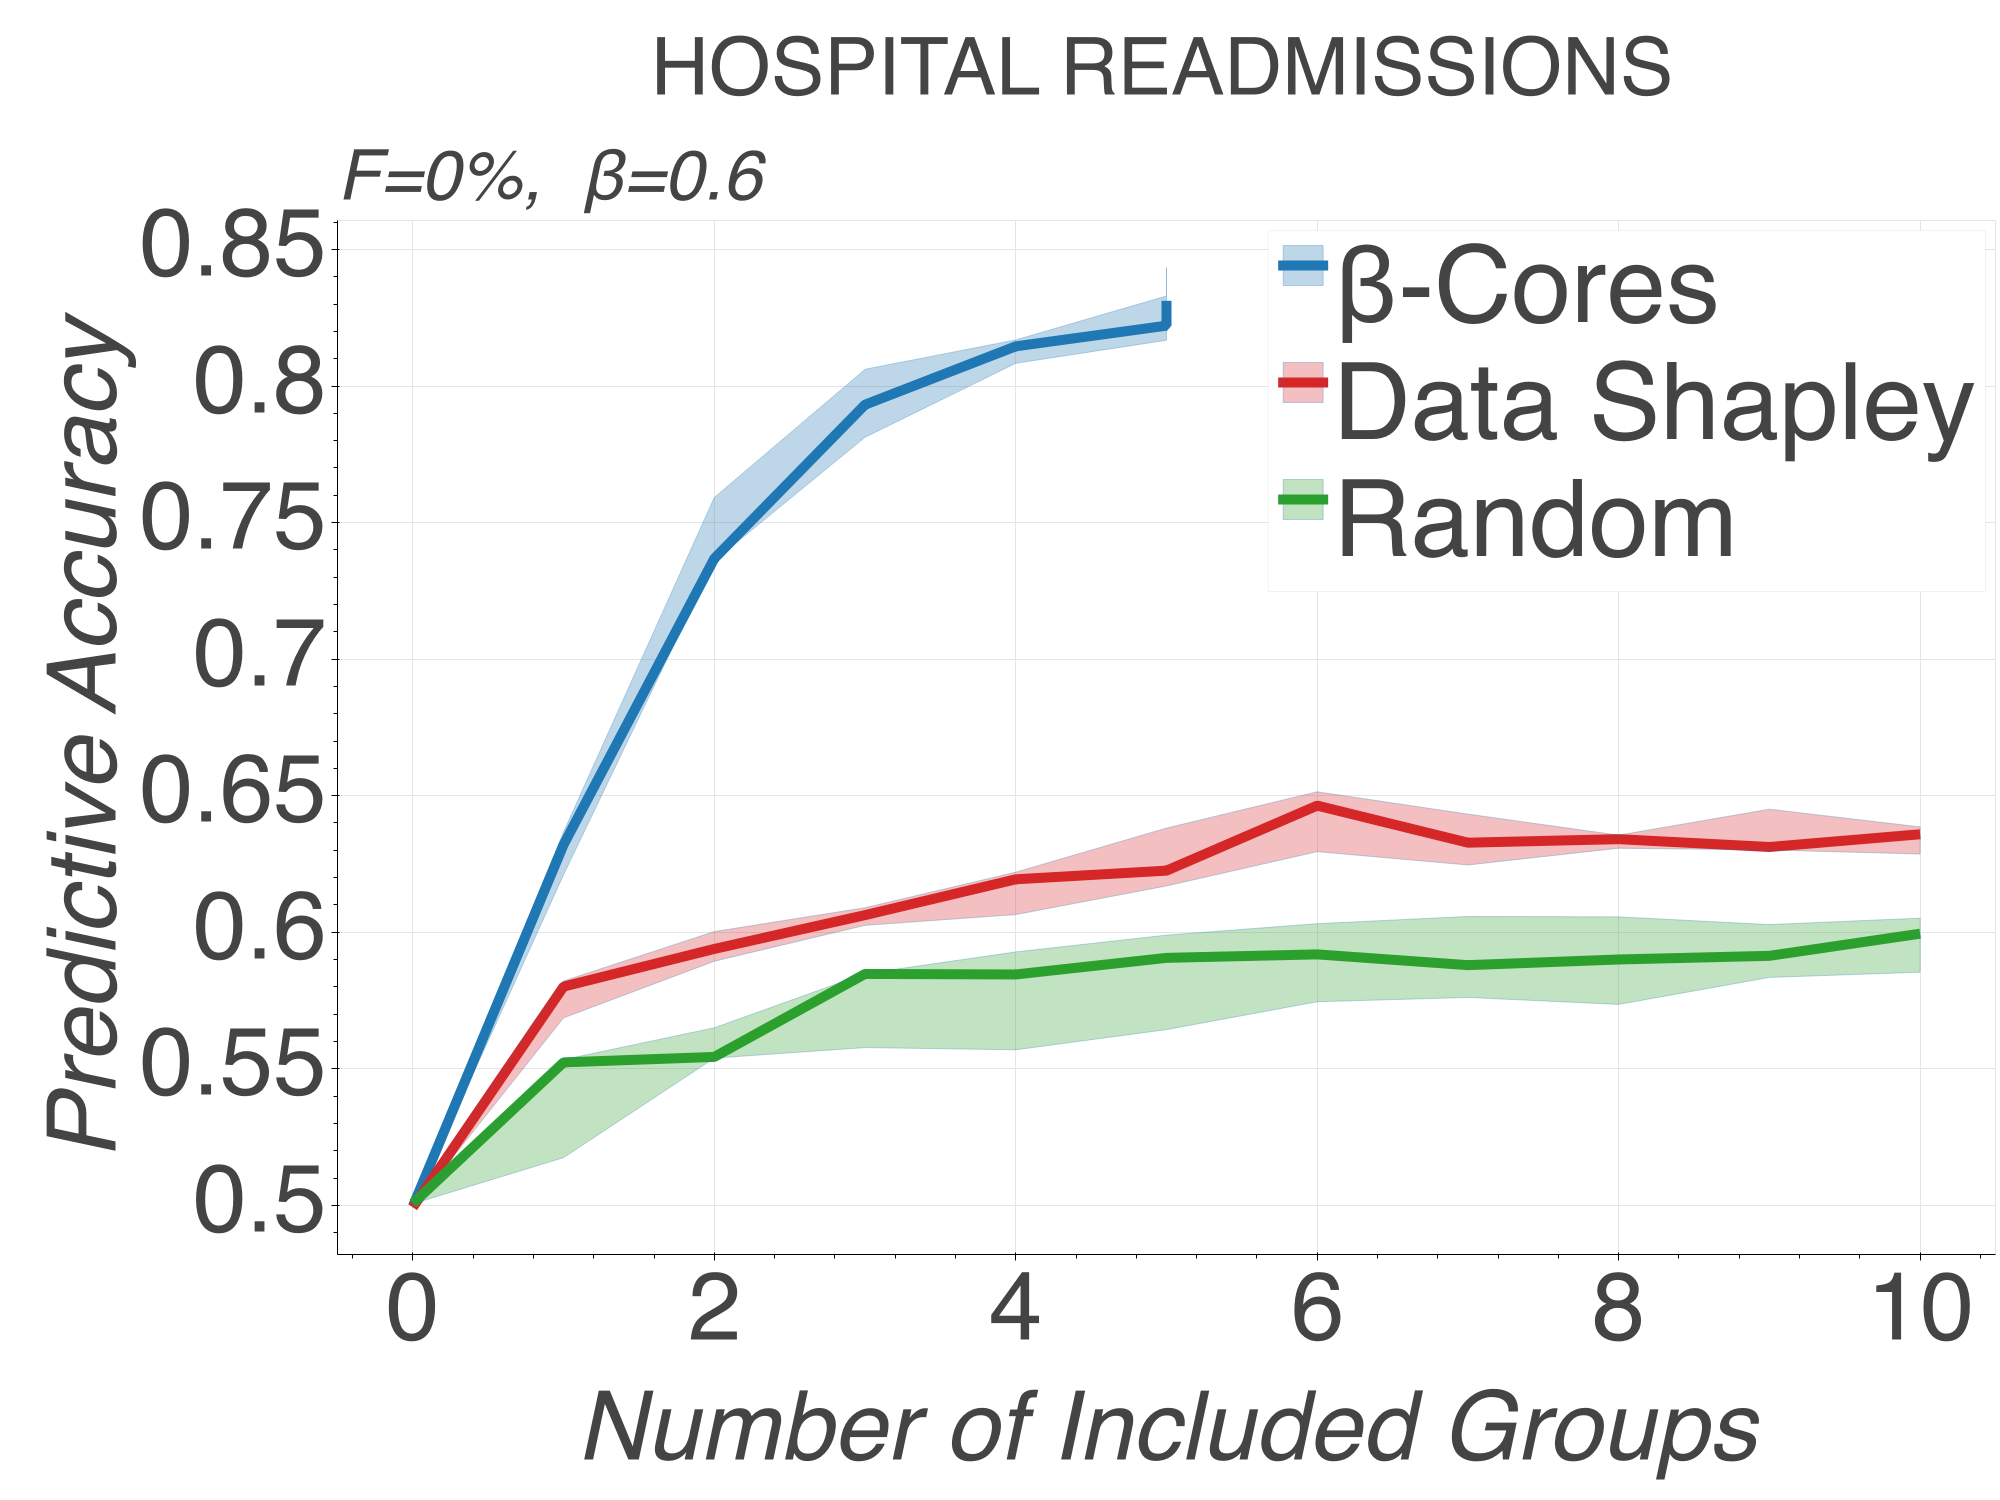
\includegraphics[width=.49\textwidth, height=3.8cm]{figs/group_diabetes06_10_0_False_ACCvsit.png}
	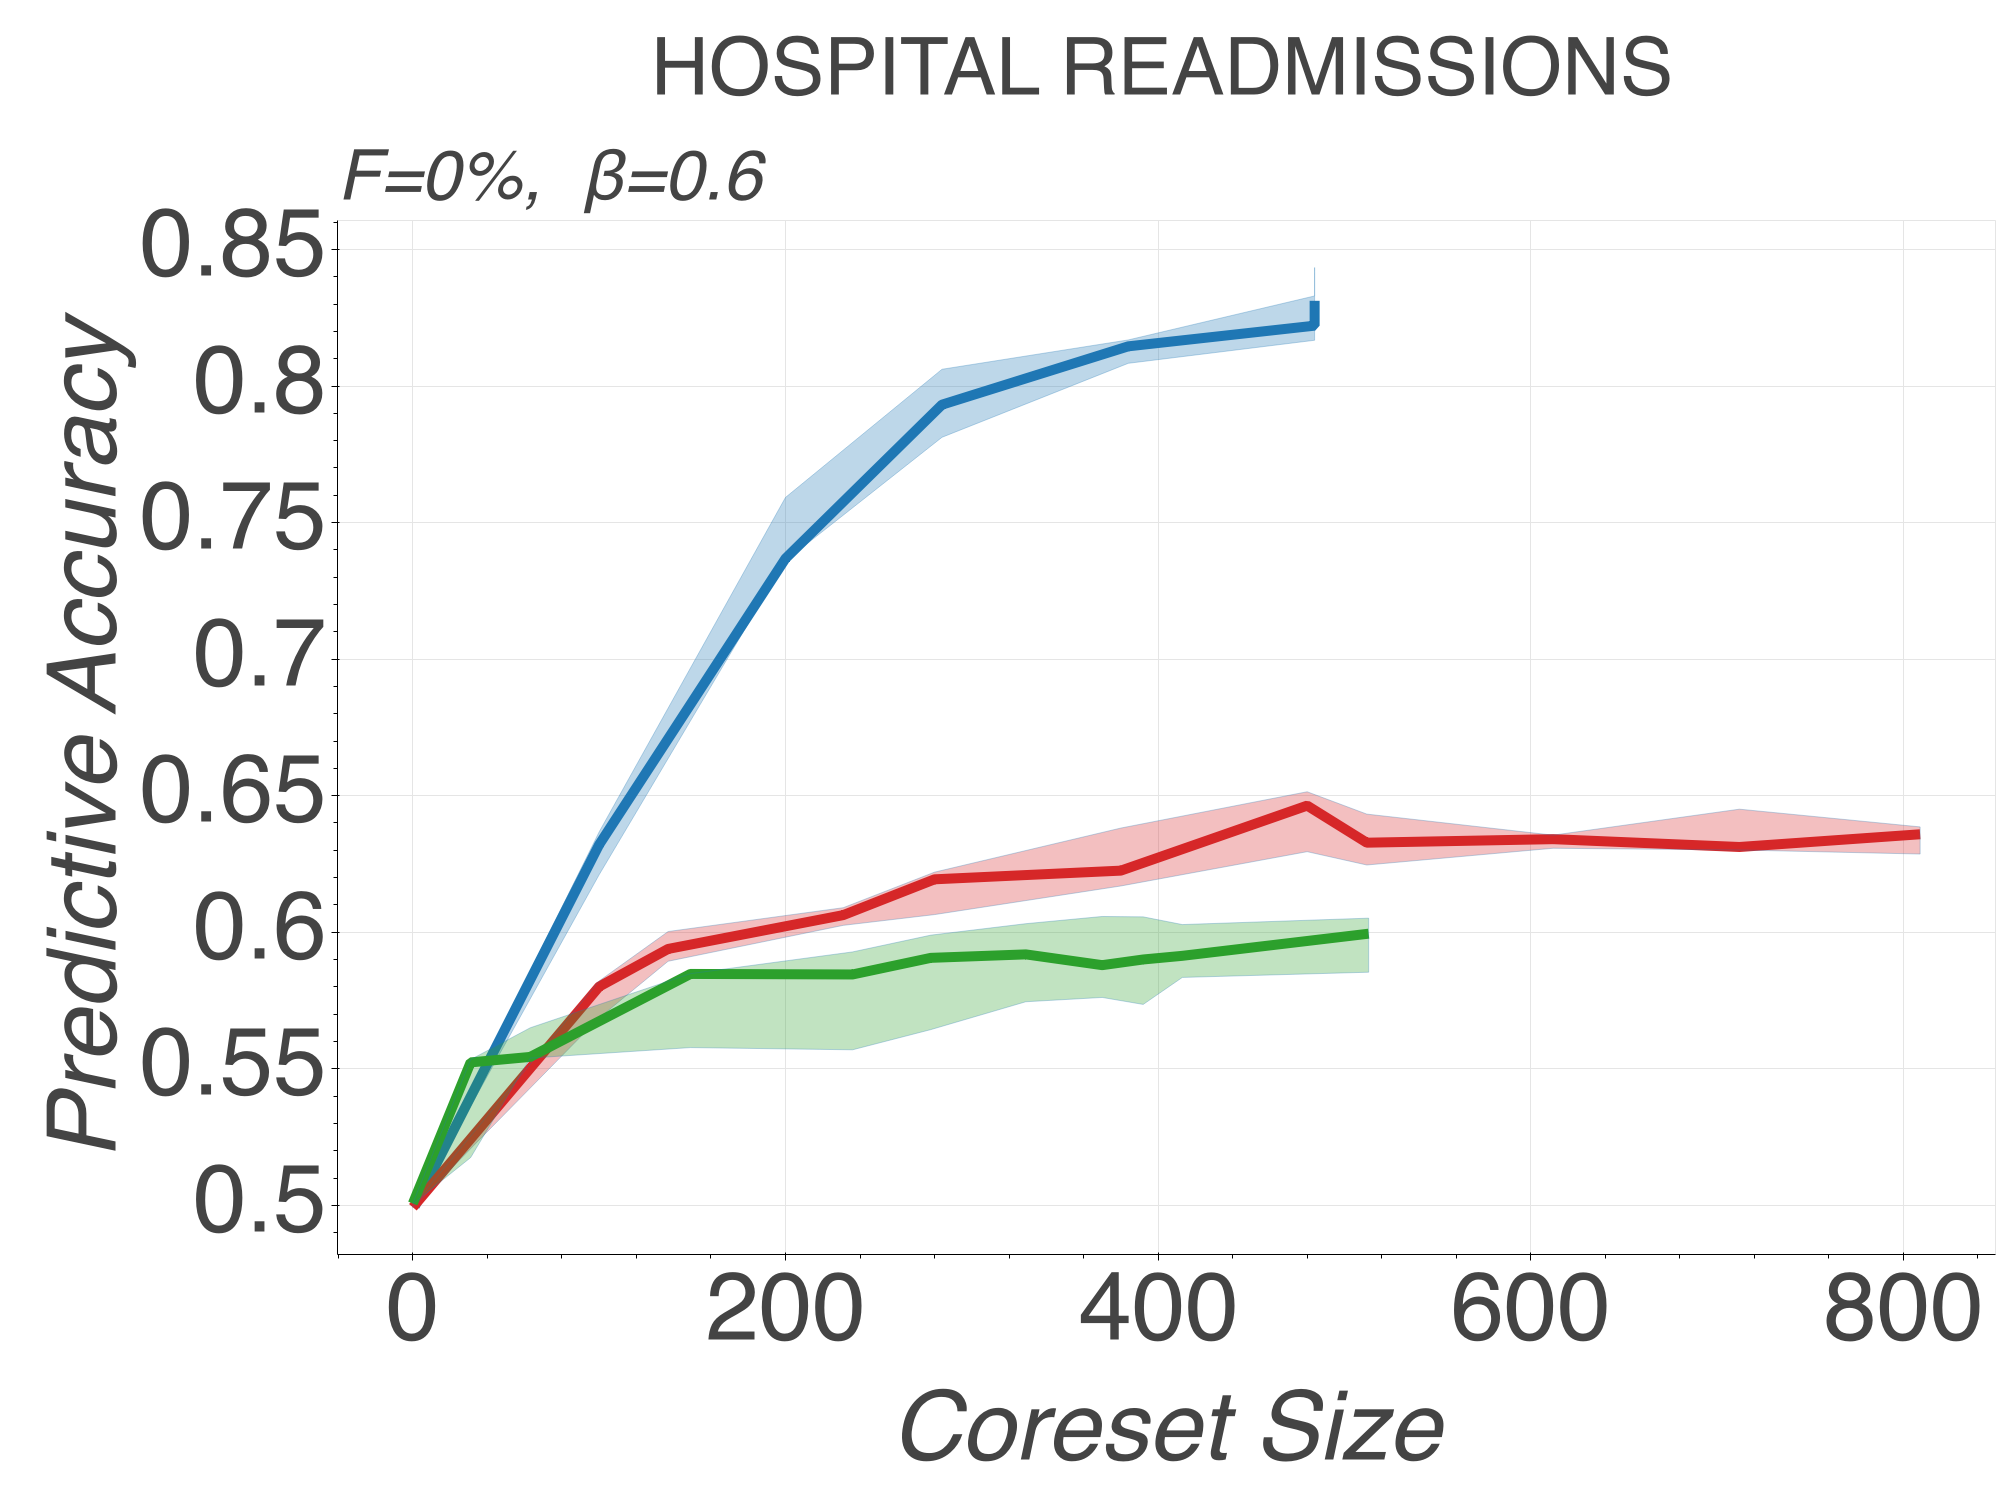
\includegraphics[width=.49\textwidth, height=3.8cm]{figs/group_diabetes06_10_0_False_ACCvssz.png}	
\end{frame}

\begin{frame}
	\frametitle{Experiment IV: Infomative Subpopulation Combinations for Budgeted Inference on Diabetes Patients' Readmissions}
	\centering
	\includegraphics[width=.49\textwidth]{figs/selected_groups.png}	
	\begin{itemize}
		\item $\blacktriangleright$ Older age Caucasian/Afro-American female group population is most informative ~\citep{ghorbani19}
		\item $\blacktriangleright$ More effective selection compared to data Shapley~\citep{shapley53}
	\end{itemize}
\end{frame}


\begin{frame}
	\frametitle{Conclusions}
	\centering
	We introduced a \\ \textbf{general-purpose  black-box} \\ Variational Inference method that \pause
	\begin{itemize}
		\item $\blacktriangleright$ addresses jointly \emph{\textbf{scalability and robustness to misspecification}} in  large-scale real-world ML applications
		\item $\blacktriangleright$ \emph{\textbf{maintains the strengths of Bayesian inference}}
		\item $\blacktriangleright$ \emph{\textbf{minimizes assumptions}} about the \emph{\textbf{model}} and the \emph{\textbf{outliers}}, and maintaining high automation
		\item $\blacktriangleright$ \emph{\textbf{preprocessing step}} compatible with black-box inference
		\item $\blacktriangleright$ points to an \emph{\textbf{efficient large-scale data subpopulations acquisition}}
	\end{itemize}
\end{frame}

\begin{frame}
	\frametitle{\textbf{Thank you!}}
	\centering
	\large{\textbf{Papers}}:\\ {https://proceedings.neurips.cc/paper/2020/\\file/ab452534c5ce28c4fbb0e102d4a4fb2e-Paper.pdf}\\{https://arxiv.org/abs/2008.13600}\\
	\vspace{1cm}
	\includegraphics[width=3.6cm,height=1.8cm]{figs/github-logo.png}\\
	\texttt{https://github.com/trevorcampbell/\\pseudocoresets-experiments}\\ \texttt{https://github.com/dionman/beta-cores}
\end{frame}


\begin{frame}[allowframebreaks]{References}
	\tiny %\scriptsize
	\bibliography{references.bib}
\end{frame}

\end{document}
